%%
%% Copyright (C) 2014 Jeffrey P. Hafner <jphafner@buffalo.edu>
%%  
%%  This program is free software: you can redistribute it and/or modify
%%  it under the terms of the GNU General Public License as published by
%%  the Free Software Foundation, either version 3 of the License, or
%%  (at your option) any later version.
%%  
%%  This program is distributed in the hope that it will be useful,
%%  but WITHOUT ANY WARRANTY; without even the implied warranty of
%%  MERCHANTABILITY or FITNESS FOR A PARTICULAR PURPOSE.  See the
%%  GNU General Public License for more details.
%%  
%%  You should have received a copy of the GNU General Public License
%%  along with this program.  If not, see <http://www.gnu.org/licenses/>.
%%

\documentclass[
    11pt,
    fleqn,
]{scrartcl}

%% to list all dependencies
%\listfiles
%\RequirePackage{snapshot}

\usepackage{AMCfull}
\newlength{\mylen}
\setlength{\parskip}{0pt} % 1ex plus 0.5ex minus 0.2ex}
\setlength{\parindent}{0pt}

\graphicspath{{./qbank/aapt/gfx/}{./qbank/nysed/gfx/}}

%% Begin Document
%%------------------------------------------------
\begin{document}

%% AAPT 52Q


%% AAPT Physics Bowl Exams Questions
%%----------------------------------------


%% This section has 58 problems


%% PhysicsBowl 2015
%%----------------------------------------
\element{aapt}{ %% Bowl-A1
\begin{question}{bowl-2015-q02}
    A box uniformly slides \SI{7.50}{\meter} to rest across
        a flat surface in a time of \SI{12.0}{\second}.
    What was the initial speed of the box when it started its slide?
    \begin{multicols}{2}
    \begin{choices}
        \wrongchoice{\SI{0.313}{\meter\per\second}}
        \wrongchoice{\SI{0.625}{\meter\per\second}}
      \correctchoice{\SI{1.25}{\meter\per\second}}
        \wrongchoice{\SI{2.50}{\meter\per\second}}
        \wrongchoice{\SI{5.00}{\meter\per\second}}
    \end{choices}
    \end{multicols}
\end{question}
}

\element{aapt}{ %% Bowl-A1
\begin{question}{bowl-2015-q06}
    A car travels at \SI{20.0}{\mile\per\hour}.
    Which one of the following choices best represents the speed
        of the car in SI units of meter per second (\si{\meter\per\second})?
    \begin{multicols}{3}
    \begin{choices}
        \wrongchoice{\SI{533}{\meter\per\second}}
        \wrongchoice{\SI{45.0}{\meter\per\second}}
        \wrongchoice{\SI{20.0}{\meter\per\second}}
      \correctchoice{\SI{8.9}{\meter\per\second}}
        \wrongchoice{\SI{0.75}{\meter\per\second}}
    \end{choices}
    \end{multicols}
\end{question}
}

\element{aapt}{ %% Bowl-A1
\begin{question}{bowl-2015-q09}
    Two cars are moving to the right on a horizontal track,
        each with constant acceleration.
    At an instant of time, the information about the cars is shown:
    \begin{description}
        \item[Car \#1:] position = \SI{125.0}{\meter};
            velocity = \SI{13.0}{\meter\per\second};
            constant acceleration = \SI{1.5}{\meter\per\second\squared}
        \item[Car \#2:] position = \SI{80.0}{\meter};
            velocity = \SI{9.30}{\meter\per\second};
            constant acceleration = \SI{5.5}{\meter\per\second\squared}
    \end{description}
    During the next \SI{1.0}{\second} of motion,
        which one of the following choices best represents
        what happens to the distance between the cars?
    \begin{choices}
        \wrongchoice{It decreases during the entire \SI{1.0}{\second} of motion.}
        \wrongchoice{It increases during the entire \SI{1.0}{\second} of motion.}
      \correctchoice{It initially increases and then decreases resulting in a greater distance between the cars after \SI{1.0}{\second}.}
        \wrongchoice{It initially increases and then decreases resulting in a smaller distance between the cars after \SI{1.0}{\second}.}
        \wrongchoice{It initially increases and then decreases resulting in the same distance between the cars after \SI{1.0}{\second}.}
    \end{choices}
\end{question}
}

\element{aapt}{ %% Bowl-A1
\begin{question}{bowl-2015-q17}
    An object starts at the origin and its velocity along a line vs. time is graphed.
    \begin{center}
    \begin{tikzpicture}
        \begin{axis}[
            axis y line=left,
            axis x line=middle,
            axis line style={->},
            xlabel={time},
            x unit=\si{\second},
            xtick={0,2,4,6,8,10},
            minor x tick num=1,
            ylabel={velocity},
            y unit=\si{\meter\per\second},
            ytick={-5,0,5},
            minor y tick num=4,
            grid=major,
            xmin=0,xmax=10.2,
            ymin=-5.5,ymax=5.5,
            width=0.95\columnwidth,
            height=0.50\columnwidth,
        ]
        \addplot[line width=1pt,mark=\empty] plot coordinates { (0,0) (3,4) (5,4) (9,-4) (10,-4) };
        \end{axis}
    \end{tikzpicture}
    \end{center}
    Which one of the following choices best gives the proper interval(s) of time for which the object is moving away from the origin?
    \begin{choices}
        \wrongchoice{Only for times $\SI{0}{\second}<t<\SI{3}{\second}$}
        \wrongchoice{Only for times $\SI{0}{\second}<t<\SI{5}{\second}$}
        \wrongchoice{Only for times $\SI{3}{\second}<t<\SI{5}{\second}$}
      \correctchoice{Only for times $\SI{0}{\second}<t<\SI{7}{\second}$}
        \wrongchoice{For times $\SI{0}{\second}<t<\SI{3}{\second}$ and $\SI{5}{\second}<t<\SI{9}{\second}$}
    \end{choices}
\end{question}
}

\element{aapt}{ %% Bowl-A1
\begin{question}{bowl-2015-q32}
    An object moving along a line completes a \SI{20.0}{\second}
        trip with an average speed of \SI{10.0}{\meter\per\second} in two stages.
    During stage 1, the object moves with a constant velocity of
        \SI{6.0}{\meter\per\second} to the right for \SI{12.0}{\second}.
    What constant magnitude acceleration directed to the left
        must the object have during the \SI{8.0}{\second} of stage 2?
    \begin{multicols}{2}
    \begin{choices}
        \wrongchoice{\SI{2.5}{\meter\per\second\squared}}
        \wrongchoice{\SI{2.7}{\meter\per\second\squared}}
        \wrongchoice{\SI{4.0}{\meter\per\second\squared}}
      \correctchoice{\SI{5.3}{\meter\per\second\squared}}
        \wrongchoice{\SI{6.3}{\meter\per\second\squared}}
    \end{choices}
    \end{multicols}
\end{question}
}

\newcommand{\BowlTwentyFifteenQFortyOne}{
\begin{tikzpicture}
    \begin{axis}[
        axis y line=left,
        axis x line=bottom,
        axis line style={->},
        xlabel={time},
        xtick={0,5,10},
        xticklabels={$0$,$T$,$2T$},
        ylabel={position},
        ytick=\empty,
        grid=major,
        xmin=0,xmax=11,
        ymin=0,ymax=20,
        width=0.95\columnwidth,
        height=0.50\columnwidth,
        very thin,
        legend style={
            at={(0.90,0.1)},
            anchor=south,
        },
        colormap={mymap}{rgb=(0,0,0); rgb=(0,0,0)}
    ]
    \addplot[dashed,line width=1pt,domain=0:10]{4+(8*x/5)};
    \addplot[line width=1pt,black,draw=black,color=black,patch,patch type=quadratic spline] coordinates {
        (0,4) (5,12) (2,2.0) (5,12) (10,20) (7,18) };
    %\legend{Truck,Car}; node??
    \end{axis}
\end{tikzpicture}
}

\element{aapt}{ %% Bowl-A1
\begin{question}{bowl-2015-q41}
    %Questions 41--42 deal with the following information:
    A car (solid line) and a truck (dashed line) are moving on a horizontal track.
    The position vs. time graph for the two vehicles is shown.
    \begin{center}
        \BowlTwentyFifteenQFortyOne
    \end{center}
    For the entire time shown in the graph,
        which one of the following choices correctly describes the relationship
        between the average speed of the truck to that of the car?
    \begin{choices}
      \correctchoice{The truck's average speed is less than the average speed of the car.}
        \wrongchoice{The truck's average speed is the same as the average speed of the car.}
        \wrongchoice{The truck's average speed is greater than the average speed of the car.}
        \wrongchoice{The truck's average speed is positive while the car's average speed is negative but of the same magnitude.}
        \wrongchoice{A relationship cannot be determined without more information.}
    \end{choices}
\end{question}
}

\element{aapt}{ %% Bowl-A1
\begin{question}{bowl-2015-q42}
    %Questions 41--42 deal with the following information:
    A car (solid line) and a truck (dashed line) are moving on a horizontal track.
    The position vs. time graph for the two vehicles is shown.
    \begin{center}
        \BowlTwentyFifteenQFortyOne
    \end{center}
    Which one of the following choices best describes the instants of time, $t$,
        at which the car and truck travel with the same speed?
    \begin{choices}
        \wrongchoice{Only at times $t=0$, $t=T$ and $t=2T$.}
        \wrongchoice{At one instant during the interval $0 < t < T$ and at one instant during the interval $T < t < 2T$.}
      \correctchoice{At two instants during the interval $0 < t < T$ and at one instant during the interval $T < t < 2T$.}
        \wrongchoice{At one instant during the interval $0 < t < T$ and at two instants during the interval $T < t < 2T$.}
        \wrongchoice{At two instants during the interval $0 < t < T$ and at two instants during the interval $T < t < 2T$.}
    \end{choices}
\end{question}
}


%% PhysicsBowl 2014
%%----------------------------------------
\element{aapt}{ %% Bowl-A1
\begin{question}{bowl-2014-q07}
    Starting from rest,
        a cart uniformly accelerates to a speed of \SI{7.60}{\meter\per\second} in a time of \SI{3.00}{\second}.
    Through what distance does the cart move in this time?
    \begin{multicols}{3}
    \begin{choices}
        \wrongchoice{\SI{5.7}{\meter}}
        \wrongchoice{\SI{8.1}{\meter}}
      \correctchoice{\SI{11.4}{\meter}}
        \wrongchoice{\SI{16.1}{\meter}}
        \wrongchoice{\SI{22.8}{\meter}}
    \end{choices}
    \end{multicols}
\end{question}
}

\element{aapt}{ %% Bowl-A1
\begin{question}{bowl-2014-q16}
    A toy car initially moves to the right at \SI{60.0}{\centi\meter\per\second}.
    Five seconds later, the car is moving at \SI{40.0}{\centi\meter\per\second} to the left.
    The total displacement of the car during this time is \SI{10.0}{\centi\meter} to the left of where it started.
    %% begin question
    Which one of the following choices best represents the magnitude of the average velocity of the car during the five second motion?
    \begin{multicols}{2}
    \begin{choices}
        \wrongchoice{\SI{50.0}{\centi\meter\per\second}}
        \wrongchoice{\SI{10.0}{\centi\meter\per\second}}
        \wrongchoice{\SI{4.0}{\centi\meter\per\second}}
      \correctchoice{\SI{2.0}{\centi\meter\per\second}}
        \wrongchoice{\SI{0.40}{\centi\meter\per\second}}
    \end{choices}
    \end{multicols}
\end{question}
}

\element{aapt}{ %% Bowl-A1
\begin{question}{bowl-2014-q17}
    A toy car initially moves to the right at \SI{60.0}{\centi\meter\per\second}.
    Five seconds later, the car is moving at \SI{40.0}{\centi\meter\per\second} to the left.
    The total displacement of the car during this time is \SI{10.0}{\centi\meter} to the left of where it started.
    %% begin question
    Which one of the following choices best represents the magnitude of the average acceleration of the car during the five second motion?
    \begin{multicols}{2}
    \begin{choices}
      \correctchoice{\SI{20.0}{\centi\meter\per\second\squared}}
        \wrongchoice{\SI{4.0}{\centi\meter\per\second\squared}}
        \wrongchoice{\SI{2.0}{\centi\meter\per\second\squared}}
        \wrongchoice{\SI{0.80}{\centi\meter\per\second\squared}}
        \wrongchoice{\SI{0.40}{\centi\meter\per\second\squared}}
    \end{choices}
    \end{multicols}
\end{question}
}


\element{aapt}{ %% Bowl-A1
\begin{question}{bowl-2014-q33}
    An object moves with constant acceleration starting with velocity $v_0=\SI{5.00}{\meter\per\second}$ and ending with a velocity of $v=-\SI{1.00}{\meter\per\second}$ in a time of \SI{3.00}{\second}.
    For this motion, what is the average speed associated with the object.
    \begin{multicols}{3}
    \begin{choices}
        \wrongchoice{\SI{2.00}{\meter\per\second}}
      \correctchoice{\SI{2.17}{\meter\per\second}}
        \wrongchoice{\SI{2.50}{\meter\per\second}}
        \wrongchoice{\SI{2.83}{\meter\per\second}}
        \wrongchoice{\SI{3.00}{\meter\per\second}}
    \end{choices}
    \end{multicols}
\end{question}
}


%% PhysicsBowl 2013
%%----------------------------------------
\element{aapt}{ %% Bowl-A1
\begin{question}{bowl-2013-q17}
    A position vs. time graph of a particle moving along a horizontal axis is shown.
    \begin{center}
    \begin{tikzpicture}
        \begin{axis}[
            axis y line=left,
            axis x line=middle,
            axis line style={->},
            xlabel={time},
            x unit=\si{\second},
            xtick={0,2,4,6,8,10},
            minor xtick={1,3,5,7,9},
            ylabel={position},
            y unit=\si{\meter},
            ytick={-10,0,10},
            minor ytick={-8,-6,-4,-2,2,4,6,8},
            grid=both,
            xmin=0,xmax=10.5,
            ymin=-10.5,ymax=10.5,
            width=0.95\columnwidth,
            height=0.618\columnwidth,
        ]
        \addplot[line width=1pt,mark=\empty] plot coordinates { (0,8) (3,8) (5,0) (6,0) (8,-8) (9,-8) (10,10) };
        \end{axis}
    \end{tikzpicture}
    \end{center}
    What is the total distance traveled by the particle from $t=\SI{0}{\second}$ to $t=\SI{10}{\second}$?
    \begin{multicols}{3}
    \begin{choices}
        \wrongchoice{\SI{2}{\meter}}
        \wrongchoice{\SI{18}{\meter}}
        \wrongchoice{\SI{26}{\meter}}
      \correctchoice{\SI{34}{\meter}}
        \wrongchoice{\SI{42}{\meter}}
    \end{choices}
    \end{multicols}
\end{question}
}

\element{aapt}{ %% Bowl-A1
\begin{question}{bowl-2013-q26}
    An object moving only to the right completes a \SI{20.0}{\second} trip in two stages, I and II.
    The average speed of the entire \SI{20.0}{\second} trip is \SI{10.0}{\meter\per\second}.
    For state I, the object moves with a constant velocity of \SI{6.0}{\meter\per\second} for \SI{12.0}{\second}.
    What constant acceleration must the object have during the \SI{8.0}{\second} of stage II?
    \begin{multicols}{2}
    \begin{choices}
        \wrongchoice{\SI{2.25}{\meter\per\second\squared}}
      \correctchoice{\SI{2.50}{\meter\per\second\squared}}
        \wrongchoice{\SI{4.00}{\meter\per\second\squared}}
        \wrongchoice{\SI{6.25}{\meter\per\second\squared}}
        \wrongchoice{\SI{8.50}{\meter\per\second\squared}}
    \end{choices}
    \end{multicols}
\end{question}
}

\element{aapt}{ %% Bowl-A1
\begin{question}{bowl-2013-q32}
    An acceleration vs. time graph for an object moving along a line is shown.
    \begin{center}
    \begin{tikzpicture}
        \begin{axis}[
            axis y line=left,
            axis x line=middle,
            axis line style={->},
            xlabel={time},
            x unit=\si{\second},
            xtick={0,2,4,6,8,10},
            minor xtick={1,3,5,7,9},
            ylabel={acceleration},
            y unit=\si{\meter\per\second\squared},
            ytick={-10,0,10},
            minor ytick={-8,-6,-4,-2,2,4,6,8},
            grid=both,
            xmin=0,xmax=10.25,
            ymin=-10.5,ymax=10.5,
            width=0.95\columnwidth,
            height=0.618\columnwidth,
        ]
        \addplot[line width=1pt,domain=0:10]{8*sin(1.26*deg(x))};
        \end{axis}
    \end{tikzpicture}
    \end{center}
    The object starts from rest at time $t=\SI{0}{\second}$.
    At what time(s) does the object attain a maximum displacement from its starting position?
    \begin{choices}
        \wrongchoice{At times $t=\SI{2.5}{\second}$ and $t=\SI{7.5}{\second}$ only}
        \wrongchoice{At times $t=\SI{5.0}{\second}$ and $t=\SI{10}{\second}$ only}
        \wrongchoice{At times $t=\SI{1.25}{\second}$, $t=\SI{3.75}{\second}$,
            $t=\SI{6.25}{\second}$, and $t=\SI{8.75}{\second}$ only}
        \wrongchoice{At times $t=\SI{2.5}{\second}$, $t=\SI{5.0}{\second}$,
            $t=\SI{7.5}{\second}$, and $t=\SI{10}{\second}$ only}
      \correctchoice{At time $t=\SI{10}{\second}$ only}
    \end{choices}
\end{question}
}


%% PhysicsBowl 2012
%%----------------------------------------
\element{aapt}{ %% Bowl-A1
\begin{question}{bowl-2012-q08}
    An object of mass \SI{5.00}{\kilo\gram} moves only to the right along the $+x$-axis.
    During some time interval, the object's speed increased from \SI{4.00}{\meter\per\second} to \SI{8.00}{\meter\per\second} with a constant acceleration of \SI{2.00}{\meter\per\second\squared}.
    Through what distance does the object move during the time interval of the acceleration?
    \begin{multicols}{3}
    \begin{choices}
        \wrongchoice{\SI{2.00}{\meter}}
        \wrongchoice{\SI{4.00}{\meter}}
        \wrongchoice{\SI{8.00}{\meter}}
      \correctchoice{\SI{12.0}{\meter}}
        \wrongchoice{\SI{24.0}{\meter}}
    \end{choices}
    \end{multicols}
\end{question}
}

\element{aapt}{ %% Bowl-A1
\begin{question}{bowl-2012-q17}
    A mass moves according to the graph of position as a function of time shown below.
    \begin{center}
    \begin{tikzpicture}
        \begin{axis}[
            axis y line=left,
            axis x line=middle,
            axis line style={->},
            xlabel={time},
            x unit=\si{\second},
            xtick={0,2,4,6,8,10},
            minor xtick={1,3,5,7,9},
            ylabel={position},
            y unit=\si{\meter},
            ytick={-10,0,10},
            minor ytick={-8,-6,-4,-2,2,4,6,8},
            grid=both,
            xmin=0,xmax=10.25,
            ymin=-10.5,ymax=10.5,
            width=0.95\columnwidth,
            height=0.618\columnwidth,
        ]
        \addplot[line width=1pt,domain=0:10]{8*sin(6.28*deg(x)/10)};
        \end{axis}
    \end{tikzpicture}
    \end{center}
    Which one of the following choices correctly represents the time or time interval for which the instantaneous velocity of the mass is considered always to be negative?
    Let $t$ represent time.
    \begin{choices}
        \wrongchoice{$t=\SI{0.0}{\second}$, $t=\SI{5.0}{\second}$ and $t=\SI{10.0}{\second}$}
        \wrongchoice{$\SI{0.0}{\second}<t<\SI{2.5}{\second}$}
      \correctchoice{$\SI{2.5}{\second}<t<\SI{7.5}{\second}$}
        \wrongchoice{$\SI{5.0}{\second}<t<\SI{10.0}{\second}$}
        \wrongchoice{$\SI{2.5}{\second}<t<\SI{10.0}{\second}$}
    \end{choices}
\end{question}
}

\element{aapt}{ %% Bowl-A1
\begin{question}{bowl-2012-q29}
    A vehicle completes one lap around a circular track
        at an average speed of \SI{50}{\meter\per\second}
        and then completes a second lap at an average speed of $V$.
    The average speed of the vehicle for the completion
        of both laps was \SI{80}{\meter\per\second}.
    What was the average speed $V$ of the second lap?
    \begin{multicols}{3}
    \begin{choices}
        \wrongchoice{\SI{100}{\meter\per\second}}
        \wrongchoice{\SI{110}{\meter\per\second}}
        \wrongchoice{\SI{125}{\meter\per\second}}
        \wrongchoice{\SI{150}{\meter\per\second}}
      \correctchoice{\SI{200}{\meter\per\second}}
    \end{choices}
    \end{multicols}
\end{question}
}


%% PhysicsBowl 2011
%%----------------------------------------
\element{aapt}{ %% Bowl-A1
\begin{question}{bowl-2011-q07}
    A ball of mass $m=\SI{0.100}{\kilo\gram}$ is launched
        straight upward so that it rises to a maximum height
        of \SI{12.0}{\meter} above the launch point.
    Ignore air resistance.
    %% Start question
    Approximately how much time does it take the ball to reach
        the maximum height from its launch?
    \begin{multicols}{3}
    \begin{choices}
        \wrongchoice{\SI{0.65}{\second}}
        \wrongchoice{\SI{1.00}{\second}}
        \wrongchoice{\SI{1.20}{\second}}
      \correctchoice{\SI{1.55}{\second}}
        \wrongchoice{\SI{2.40}{\second}}
    \end{choices}
    \end{multicols}
\end{question}
}

\element{aapt}{ %% Bowl-A1
\begin{question}{bowl-2011-q08}
    An object moves along a horizontal line with increasing speed.
    Which one of the following choices could represent the signs of the velocity and of the acceleration for the object to achieve this motion?
    \begin{center}
    \begin{tabu}{cX[c]X[c]}
        \toprule
        \makebox[1.5em][c]{\textnumero}
            & Velocity & Acceleration \\
        \bottomrule
    \end{tabu}
    \end{center}
    \begin{choices}
        \wrongchoice{\begin{tabu}{X[c]X[c]} Zero & Zero \\ \end{tabu}}
        \wrongchoice{\begin{tabu}{X[c]X[c]} Positive & Zero \\ \end{tabu}}
        \wrongchoice{\begin{tabu}{X[c]X[c]} Positive & Negative \\ \end{tabu}}
        \wrongchoice{\begin{tabu}{X[c]X[c]} Negative & Positive \\ \end{tabu}}
      \correctchoice{\begin{tabu}{X[c]X[c]} Negative & Negative \\ \end{tabu}}
    \end{choices}
\end{question}
}

\element{aapt}{ %% Bowl-A1
\begin{question}{bowl-2011-q09}
    Which one of the following choices best represents the speed of \SI{60.0}{\mile\per\hour} rewritten in units of \si{\kilo\meter\per\day}?
    \begin{multicols}{2}
    \begin{choices}
      \correctchoice{\SI{2300}{\kilo\meter\per\day}}
        \wrongchoice{\SI{1440}{\kilo\meter\per\day}}
        \wrongchoice{\SI{900}{\kilo\meter\per\day}}
        \wrongchoice{\SI{4.00}{\kilo\meter\per\day}}
        \wrongchoice{\SI{1.56}{\kilo\meter\per\day}}
    \end{choices}
    \end{multicols}
\end{question}
}

\element{aapt}{ %% Bowl-A1
\begin{question}{bowl-2011-q14}
    A car makes a trip in two parts.
    \begin{description}[itemsep=0pt]
        \item[Part 1:] It travels a distance of \SI{800}{\meter} at a constant speed of \SI{4.0}{\meter\per\second}.
        \item[Part 2:] It travels a distance of \SI{1200}{\meter} at a constant speed of \SI{20.0}{\meter\per\second}.
    \end{description}
    What is the average speed of the two-part trip?
    \begin{multicols}{3}
    \begin{choices}
      \correctchoice{\SI{7.7}{\meter\per\second}}
        \wrongchoice{\SI{10.4}{\meter\per\second}}
        \wrongchoice{\SI{12.0}{\meter\per\second}}
        \wrongchoice{\SI{13.6}{\meter\per\second}}
        \wrongchoice{\SI{17.3}{\meter\per\second}}
    \end{choices}
    \end{multicols}
\end{question}
}

\newcommand{\BowlTwentyElevenQEighteen}{
\begin{tikzpicture}
    \begin{axis}[
        axis y line=left,
        axis x line=middle,
        axis line style={->},
        xlabel={time},
        x unit=\si{\second},
        xtick={0,2,4,6,8,10},
        minor x tick num=1,
        ylabel={velocity},
        y unit=\si{\meter\per\second},
        ytick={-10,0,10},
        minor y tick num=4,
        grid=both,
        xmin=0,xmax=10,
        ymin=-10,ymax=10,
        width=0.8\columnwidth,
        height=0.5\columnwidth,
    ]
    \addplot[line width=1pt,domain=0:10] { 8*sin(36*x) };
    \end{axis}
\end{tikzpicture}
}

\element{aapt}{ %% Bowl-A1
\begin{question}{bowl-2011-q18}
    The motion of an object moving along a straight line is given by the velocity vs. time graph shown.
    \begin{center}
        \BowlTwentyElevenQEighteen
    \end{center}
    Which one of the following choices best represents the average acceleration of the object during the time interval from $t=\SI{4.0}{\second}$ to $t=\SI{9.0}{\second}$?
    \begin{multicols}{2}
    \begin{choices}
        \wrongchoice{\SI{0.80}{\meter\per\second\squared}}
        \wrongchoice{\SI{0}{\meter\per\second\squared}}
        \wrongchoice{\SI{-0.80}{\meter\per\second\squared}}
      \correctchoice{\SI{-1.6}{\meter\per\second\squared}}
        \wrongchoice{\SI{-3.2}{\meter\per\second\squared}}
    \end{choices}
    \end{multicols}
\end{question}
}

\element{aapt}{ %% Bowl-A1
\begin{question}{bowl-2011-q19}
    The motion of an object moving along a straight line is given by the velocity vs. time graph shown.
    \begin{center}
        \BowlTwentyElevenQEighteen
    \end{center}
    Which one of the following choices best represents the instantaneous acceleration of the object at the time $t=\SI{4.0}{\second}$
    \begin{multicols}{2}
    \begin{choices}
        \wrongchoice{\SI{0}{\meter\per\second\squared}}
        \wrongchoice{\SI{-1.6}{\meter\per\second\squared}}
        \wrongchoice{\SI{-2.0}{\meter\per\second\squared}}
        \wrongchoice{\SI{-3.2}{\meter\per\second\squared}}
      \correctchoice{\SI{-4.0}{\meter\per\second\squared}}
    \end{choices}
    \end{multicols}
\end{question}
}

%% NOTE: bowl-2011-q21?

\element{aapt}{ %% Bowl-A1
\begin{question}{bowl-2011-q30}
    Two cars travel to the right, each starting from rest, along a straight road.
    Car $A$ has twice the acceleration of car $B$.
    After traveling a distance $d$, Car $A$ has speed $v$.
    When Car $B$ has traveled the same distance $d$, what is its speed in terms of $v$?
    \begin{multicols}{3}
    \begin{choices}
        \wrongchoice{$\dfrac{1}{4}v$}
        \wrongchoice{$\dfrac{1}{2}v$}
        \wrongchoice{$\dfrac{\sqrt{3}}{2}v$}
      \correctchoice{$\dfrac{\sqrt{2}}{2}v$}
        \wrongchoice{$v$}
    \end{choices}
    \end{multicols}
\end{question}
}


%% PhysicsBowl 2010
%%----------------------------------------
\element{aapt}{ %% Bowl-A1
\begin{question}{bowl-2010-q04}
    Which of the following relationships correctly ranks
        the three given speeds from least to greatest?
    The speeds are given as $v_1=\SI{1.25e-4}{\centi\meter\per\micro\second}$,
        $v_2=\SI{0.076}{\mega\meter\per\week}$,
        $v_3=\SI{9.50}{\kilo\meter\per\day}$.
    \begin{multicols}{2}
    \begin{choices}
        \wrongchoice{$v_1<v_2<v_3$}
      \correctchoice{$v_3<v_2<v_1$}
        \wrongchoice{$v_2<v_3<v_1$}
        \wrongchoice{$v_1<v_3<v_2$}
        \wrongchoice{$v_3<v_2=v_1$}
    \end{choices}
    \end{multicols}
\end{question}
}

\element{aapt}{ %% Bowl-A1
\begin{question}{bowl-2010-q07}
    A small object is thrown straight downward on Earth with
        an initial speed of \SI{12.0}{\meter\per\second}
        from a position \SI{10.0}{\meter} above the ground.
    Ignoring air resistance, the speed of the object when it reaches the ground is:
    \begin{multicols}{3}
    \begin{choices}
      \correctchoice{\SI{18.4}{\meter\per\second}}
        \wrongchoice{\SI{14.6}{\meter\per\second}}
        \wrongchoice{\SI{14.0}{\meter\per\second}}
        \wrongchoice{\SI{12.8}{\meter\per\second}}
        \wrongchoice{\SI{12.0}{\meter\per\second}}
    \end{choices}
    \end{multicols}
\end{question}
}

\element{aapt}{ %% Bowl-A1
\begin{question}{bowl-2010-q10}
    A particle travels at a constant speed around
        a circular path of radius $R$.
    If the particle makes one complete trip around
        the entire circle, what is the magnitude
        of the displacement for this trip?
    \begin{multicols}{3}
    \begin{choices}
        \wrongchoice{$\pi R$}
        \wrongchoice{$2 R$}
        \wrongchoice{$2\pi R$}
        \wrongchoice{$\pi R^2$}
      \correctchoice{zero}
        %% NOTE: added for symmetry
        %\wrongchoice{$4\pi R$}
    \end{choices}
    \end{multicols}
\end{question}
}

\element{aapt}{ % Bowl-A1
\begin{question}{bowl-2010-q11}
    Consider the motion of an object given by the velocity
        vs. time graph shown below.
    \begin{center}
    \begin{tikzpicture}
        \begin{axis}[
            axis y line=left,
            axis x line=middle,
            axis line style={->},
            xlabel={time},
            x unit=\si{\second},
            xtick={0,2,4,6,8,10},
            minor x tick num=1,
            ylabel={velocity},
            y unit=\si{\meter\per\second},
            ytick={-10,0,10},
            minor y tick num=4,
            grid=both,
            xmin=0,xmax=10,
            ymin=-10,ymax=10,
            width=0.95\columnwidth,
            height=0.50\columnwidth,
        ]
        \addplot[mark=\empty,smooth] plot coordinates { (0,-6) (5,8) (10,-8) };
        \end{axis}
    \end{tikzpicture}
    \end{center}
    For which time(s) is the acceleration of the object
        equal to \SI{0}{\meter\per\second\squared}?
    \begin{choices}
        \wrongchoice{Only at time $t=\SI{2.0}{\second}$}
      \correctchoice{Only at time $t=\SI{5.0}{\second}$}
        \wrongchoice{Only at time $t=\SI{8.0}{\second}$}
        \wrongchoice{At times $t=\SI{2.0}{\second}$ and $t=\SI{5.0}{\second}$}
        \wrongchoice{At times $t=\SI{2.0}{\second}$, $t=\SI{5.0}{\second}$, and $t=\SI{8.0}{\second}$}
    \end{choices}
\end{question}
}

\element{aapt}{ %% Bowl-A1
\begin{question}{bowl-2010-q24}
    By computing the area under the acceleration vs time
        graph for a fixed time interval of an object's
        motion, what quantity has been determined for that object?
    \begin{choices}
        \wrongchoice{The average velocity during the time interval.}
        \wrongchoice{The velocity at the end of the time interval.}
        \wrongchoice{The average speed during the time interval.}
      \correctchoice{The change in velocity during the time interval.}
        \wrongchoice{The velocity at the time midway through the time interval.}
    \end{choices}
\end{question}
}

\element{aapt}{ %% Bowl-A1
\begin{question}{bowl-2010-q29}
    A ball initially at rest falls without air resistance from
        a height $h$ above the ground.
    If the ball falls the first distance $\frac{h}{2}$ in a time
        $t$, how much time is required to fall the remaining
        distance of $\frac{h}{2}$?
    \begin{multicols}{3}
    \begin{choices}
        \wrongchoice{$\num{0.25}t$}
      \correctchoice{$\num{0.41}t$}
        \wrongchoice{$\num{0.50}t$}
        \wrongchoice{$\num{0.71}t$}
        \wrongchoice{$\num{1.00}t$}
    \end{choices}
    \end{multicols}
\end{question}
}

\element{aapt}{ %% Bowl-A1
\begin{question}{bowl-2010-q38}
    Two objects both move uniformly accelerate to the right.
    At time $t=\SI{0}{\second}$, the objects are at the same
        initial position but
    \begin{itemize}
        \item Object 1 has initial speed twice that of Object 2
        \item Object 1 has one-half the acceleration of Object 2
    \end{itemize}
    After some time $T$, the velocity of the two objects is the same.
    What is the ratio of the distance traveled in this time $T$
        by Object 2 to that traveled by Object 1?
    \begin{multicols}{3}
    \begin{choices}
        \wrongchoice{$5:6$}
      \correctchoice{$4:5$}
        \wrongchoice{$3:4$}
        \wrongchoice{$2:3$}
        \wrongchoice{$1:2$}
    \end{choices}
    \end{multicols}
\end{question}
}


%% PhysicsBowl 2009
%%----------------------------------------

%% NOTE: bowl-2009-q08

\element{aapt}{ %% Bowl-A1
\begin{question}{bowl-2009-q17}
    A toy car moves \SI{3.0}{\meter} to the North in \SI{1.0}{\second}.
    The car then moves at \SI{9.0}{\meter\per\second} due South
        for \SI{2.0}{\second}.
    What is the average speed of the car for this \SI{3.0}{\second} trip?
    \begin{multicols}{3}
    \begin{choices}
        \wrongchoice{\SI{4.0}{\meter\per\second}}
        \wrongchoice{\SI{5.0}{\meter\per\second}}
        \wrongchoice{\SI{6.0}{\meter\per\second}}
      \correctchoice{\SI{7.0}{\meter\per\second}}
        \wrongchoice{\SI{12.0}{\meter\per\second}}
    \end{choices}
    \end{multicols}
\end{question}
}

\element{aapt}{ %% Bowl-A1
\begin{question}{bowl-2009-q31}
    A car moves to the right along a one-dimensional track
        for a total time $T$ in two parts.
    \begin{description}
        \item[Part One:] The car maintains constant non-zero speed $V$
            for the first \num{3/4} of the total time.
        \item[Part Two:] The car accelerates uniformly to rest during
                the last \num{1/4} of the total time.
    \end{description}
    What is the ratio of the distance traveled during Part One of
        the trip to the distance traveled during Part Two of the trip?
    \begin{multicols}{2}
    \begin{choices}
      \correctchoice{$6:1$}
        \wrongchoice{$3:2$}
        \wrongchoice{$4:3$}
        \wrongchoice{$8:3$}
        \wrongchoice{The values of $V$ and $T$ are required to answer the question.}
    \end{choices}
    \end{multicols}
\end{question}
}


%% PhysicsBowl 2008
%%----------------------------------------
\element{aapt}{ %% Bowl-A1
\begin{question}{bowl-2008-q03}
    A dog starts from rest and runs in a straight line
        with constant acceleration of \SI{2.5}{\meter\per\second\squared}.
    How much time does it take for the dog to run
        a distance of \SI{10.0}{\meter}?
    \begin{multicols}{3}
    \begin{choices}
        \wrongchoice{\SI{8.0}{\second}}
        \wrongchoice{\SI{4.0}{\second}}
      \correctchoice{\SI{2.8}{\second}}
        \wrongchoice{\SI{2.0}{\second}}
        \wrongchoice{\SI{1.4}{\second}}
    \end{choices}
    \end{multicols}
\end{question}
}

\newcommand{\BowlTwentyZeroEightQTwentyThree}{
\begin{tikzpicture}
    \begin{axis}[
        axis y line=left,
        axis x line=middle,
        axis line style={->},
        xlabel={time},
        x unit=\si{\second},
        xtick={0,2,4,6,8,10},
        minor x tick num=1,
        ylabel={velocity},
        y unit=\si{\meter\per\second},
        ytick={-10,-5,0,5,10},
        minor y tick num=4,
        grid=major,
        xmin=0,xmax=10,
        ymin=-10,ymax=10,
        width=0.95\columnwidth,
        height=0.618\columnwidth,
    ]
    \addplot[line width=1pt,domain=0:3]{8};
    \addplot[line width=1pt,domain=3:6]{20 - 4*x};
    \addplot[line width=1pt,domain=6:10]{-4};
    \end{axis}
\end{tikzpicture}
}

\element{aapt}{ %% Bowl-A1
\begin{question}{bowl-2008-q23}
    The velocity vs. time graph for the motion of a car on a straight track is shown in the diagram.
    The thick line represents the velocity.
    Assume that the car starts at the origin $x=0$.
    \begin{center}
        \BowlTwentyZeroEightQTwentyThree
    \end{center}
    At which time is the car the greatest distance from the origin?
    \begin{multicols}{3}
    \begin{choices}
        \wrongchoice{$t=\SI{10}{\second}$}
        \wrongchoice{$t=\SI{6}{\second}$}
      \correctchoice{$t=\SI{5}{\second}$}
        \wrongchoice{$t=\SI{3}{\second}$}
        \wrongchoice{$t=\SI{0}{\second}$}
    \end{choices}
    \end{multicols}
\end{question}
}

\element{aapt}{ %% Bowl-A1
\begin{question}{bowl-2008-q24}
    The velocity vs. time graph for the motion of a car on a straight track is shown in the diagram.
    The thick line represents the velocity.
    Assume that the car starts at the origin $x=0$.
    \begin{center}
        \BowlTwentyZeroEightQTwentyThree
    \end{center}
    What is the average speed of the car for the \SI{10}{\second} interval?
    \begin{multicols}{3}
    \begin{choices}
        \wrongchoice{\SI{1.20}{\meter\per\second}}
        \wrongchoice{\SI{1.40}{\meter\per\second}}
        \wrongchoice{\SI{3.30}{\meter\per\second}}
      \correctchoice{\SI{5.00}{\meter\per\second}}
        \wrongchoice{\SI{5.40}{\meter\per\second}}
    \end{choices}
    \end{multicols}
\end{question}
}


%% PhysicsBowl 2007
%%----------------------------------------
\element{aapt}{ %% Bowl-A1
\begin{question}{bowl-2007-q03}
    Two automobiles are \SI{150}{\kilo\meter} apart and traveling toward each other.
    One automobile is moving at \SI{60}{\kilo\meter\per\hour} and the other is moving \SI{40}{\kilo\meter\per\hour}.
    In how many hours will they meet?
    \begin{multicols}{3}
    \begin{choices}
      \correctchoice{\SI{1.5}{\hour}}
        \wrongchoice{\SI{1.75}{\hour}}
        \wrongchoice{\SI{2.0}{\hour}}
        \wrongchoice{\SI{2.5}{\hour}}
        \wrongchoice{\SI{3.0}{\hour}}
    \end{choices}
    \end{multicols}
\end{question}
}

\element{aapt}{ %% Bowl-A1
\begin{questionmult}{bowl-2007-q04}
    A particle moves on the $x$-axis.
    When the particle's acceleration is positive and increasing
    \begin{choices}
        \wrongchoice{its velocity must be positive.}
        \wrongchoice{its velocity must be negative.}
        \wrongchoice{it must be slowing down.}
        \wrongchoice{it must be speeding up.}
        %\correctchoice{none of the other options are true.}
    \end{choices}
\end{questionmult}
}

\element{aapt}{ %% Bowl-A1
\begin{question}{bowl-2007-q05}
    The position-time, $y$ vs. $t$, graph for the motion
        of an object is shown.
    \begin{center}
    \begin{tikzpicture}
        \begin{axis}[
            axis y line=left,
            axis x line=bottom,
            axis line style={->},
            xlabel={time},
            x unit=\si{\second},
            xtick={0,1,2,3,4,5},
            minor x tick num=1,
            ylabel={position},
            y unit=\si{\meter},
            ytick={0,10,20,30},
            minor y tick num=4,
            grid=major,
            xmin=0,xmax=5.2,
            ymin=0,ymax=32,
            width=0.95\columnwidth,
            height=0.50\columnwidth,
        ]
        \addplot[line width=1pt,domain=0:5]{25 - 4*(x-2.5)*(x-2.5)};
        \end{axis}
    \end{tikzpicture}
    \end{center}
    What would be a reasonable equation for the acceleration $a$ that would account for this motion?
    \begin{choices}
        \wrongchoice{$a=0$}
        \wrongchoice{$a=$ positive constant}
      \correctchoice{$a=$ negative constant}
        \wrongchoice{$a=$ positive constant times $t$}
        \wrongchoice{$a=$ negative constant times $t$}
    \end{choices}
\end{question}
}

\element{aapt}{ %% Bowl-A1
\begin{question}{bowl-2007-q08}
    What does one obtain by dividing the distance of \SI{12}{\mega\meter} by the time of \SI{4}{\tera\second}?
    \begin{multicols}{3}
    \begin{choices}
        \wrongchoice{\SI{3}{\nano\meter\per\second}}
      \correctchoice{\SI{3}{\micro\meter\per\second}}
        \wrongchoice{\SI{3}{\milli\meter\per\second}}
        \wrongchoice{\SI{3}{\kilo\meter\per\second}}
        \wrongchoice{\SI{3}{\giga\meter\per\second}}
    \end{choices}
    \end{multicols}
\end{question}
}

\element{aapt}{ %% Bowl-A1
\begin{question}{bowl-2007-q11}
    A cart is initially moving at \SI{0.5}{\meter\per\second} along a track.
    The cart comes to rest after traveling \SI{1}{\meter}.
    The experiment is repeated on the same track,
        but now the cart is initially moving at \SI{1}{\meter\per\second}.
    How far does the cart travel before coming to rest?
    \begin{multicols}{3}
    \begin{choices}
        \wrongchoice{\SI{1}{\meter}}
        \wrongchoice{\SI{2}{\meter}}
        \wrongchoice{\SI{3}{\meter}}
      \correctchoice{\SI{4}{\meter}}
        \wrongchoice{\SI{5}{\meter}}
    \end{choices}
    \end{multicols}
\end{question}
}

\element{aapt}{ %% Bowl-A1
\begin{question}{bowl-2007-q12}
    The definition of average velocity is:
    \begin{choices}
        \wrongchoice{the average acceleration multiplied by the time.}
        \wrongchoice{distance traveled divided by the time.}
        \wrongchoice{$\frac{1}{2}\left(v_f+v_i\right)$}
        \wrongchoice{radius multiplied by angular velocity.}
      \correctchoice{displacement divided by the time.}
    \end{choices}
\end{question}
}


%% PhysicsBowl 2006
%%----------------------------------------
\element{aapt}{ %% Bowl-A1
\begin{question}{bowl-2006-q03}
    Three students were arguing about the height of a parking garage.
    One student suggested that to determine the height of the garage,
        they simply had to drop tennis balls from the top and time
        the fall of the tennis balls.
    If the time for the ball to fall was \SI{1.4}{\second},
        approximately how tall is the parking garage?
    \begin{multicols}{3}
    \begin{choices}
        \wrongchoice{\SI{4.9}{\meter}}
        \wrongchoice{\SI{7.0}{\meter}}
      \correctchoice{\SI{9.8}{\meter}}
        \wrongchoice{\SI{13.8}{\meter}}
        \wrongchoice{\SI{19.6}{\meter}}
    \end{choices}
    \end{multicols}
\end{question}
}

\element{aapt}{ %% Bowl-A1
\begin{question}{bowl-2006-q07}
    A car has the velocity versus time curve shown.
    %% NOTE: bowl-2007-q17
    \begin{center}
    \begin{tikzpicture}
        \begin{axis}[
            axis y line=left,
            axis x line=middle,
            axis line style={->},
            clip=false,
            xlabel={time},
            x unit=\si{\second},
            xtick={0,1,2,3,4,5,6},
            ylabel={velocity},
            y unit=\si{\meter\per\second},
            ytick={-10,0,10},
            minor y tick num=1,
            grid=major,
            xmin=0,xmax=6.5,
            ymin=-15,ymax=15,
            width=0.8\columnwidth,
            height=0.5\columnwidth,
        ]
        \addplot[very thick,smooth,tension=0.7,mark=\empty] plot coordinates { (0,0) (1,6) (2,15) (3,7) (3.3,0) (4,-10) (5.1,0) (5,-1) (6,6) };
        \end{axis}
    \end{tikzpicture}
    \end{center}
    Which of the following statements regarding its motion is \emph{incorrect}?
    \begin{choices}
        \wrongchoice{The car is moving fastest at \SI{2.0}{\second}.}
        \wrongchoice{The car is at rest at approximately \SI{5.2}{\second}.}
        \wrongchoice{The car is speeding up from $t=\SI{0}{\second}$ to $t=\SI{2.0}{\second}$.}
      \correctchoice{The car has negative acceleration at $t=\SI{4.5}{\second}$.}
        \wrongchoice{The car has no acceleration at the instant $t=\SI{2.0}{\second}$.}
    \end{choices}
\end{question}
}

\element{aapt}{ %% Bowl-A1
\begin{question}{bowl-2006-q18}
    A cart is initially moving at \SI{0.5}{\meter\per\second} along a track.
    The cart comes to rest after traveling \SI{1}{\meter}.
    The experiment is repeated on the same track,
        but now the cart is initially moving at \SI{1}{\meter\per\second}.
    How far does the cart travel before coming to rest?
    \begin{multicols}{3}
    \begin{choices}
        \wrongchoice{\SI{1}{\meter}}
        \wrongchoice{\SI{2}{\meter}}
        \wrongchoice{\SI{3}{\meter}}
      \correctchoice{\SI{4}{\meter}}
        \wrongchoice{\SI{8}{\meter}}
    \end{choices}
    \end{multicols}
\end{question}
}


%% PhysicsBowl 2005
%%----------------------------------------
\element{aapt}{ %% Bowl-A1
\begin{question}{bowl-2005-q07}
    A snail is moving along a straight line.
    Its initial position is $x_0 = \SI{-5}{\meter}$ and it is moving away from the origin and slowing down.
    In this coordinate system, the signs of the initial position $x_0$,
        initial velocity $v_0$ and acceleration $a$, respectively, are
    \begin{choices}
        \wrongchoice{$x_0=-$, $v_0=+$, $a=+$}
      \correctchoice{$x_0=-$, $v_0=-$, $a=+$}
        \wrongchoice{$x_0=-$, $v_0=-$, $a=-$}
        \wrongchoice{$x_0=-$, $v_0=+$, $a=-$}
        \wrongchoice{$x_0=+$, $v_0=+$, $a=+$}
    \end{choices}
\end{question}
}


%% PhysicsBowl 2000
%%----------------------------------------
\element{aapt}{ %% Bowl-A1
\begin{question}{bowl-2000-q09}
    Is it possible for an object's velocity to increase while its acceleration decreases?
    \begin{choices}
        \wrongchoice{No, this is impossible because of the way in which acceleration is defined.}
        \wrongchoice{No, because if acceleration is decreasing the object will be slowing down.}
        \wrongchoice{No, because velocity and acceleration must always be in the same direction.}
        \wrongchoice{Yes, an example would be a falling object near the surface of the moon.}
      \correctchoice{Yes, an example would be a falling object in the presence of air resistance}
    \end{choices}
\end{question}
}

\element{aapt}{ %% Bowl-A1
\begin{question}{bowl-2000-q40}
    Suppose two cars are racing on a circular track \SI{1}{\kilo\meter} in circumference.
    The first car can circle the track in \SI{15}{\second} at top speed
        while the second car can circle the track in \SI{12}{\second} at top speed.
    How much lead does the first car need starting the last lap of the race not to lose?
    \begin{multicols}{2}
    \begin{choices}
      \correctchoice{at least \SI{250}{\meter}}
        \wrongchoice{at least \SI{200}{\meter}}
        \wrongchoice{at least \SI{104}{\meter}}
        \wrongchoice{at least \SI{83}{\meter}}
        \wrongchoice{at least \SI{67}{\meter}}
    \end{choices}
    \end{multicols}
\end{question}
}


%% PhysicsBowl 1999
%%----------------------------------------
\element{aapt}{ %% Bowl-A1
\begin{question}{bowl-1999-q01}
    %% NOTE: NIST style convention is distance divied by time
    The change of distance per unit time without reference
        to a particular direction is called
    \begin{multicols}{2}
    \begin{choices}
        \wrongchoice{inertia}
      \correctchoice{speed}
        \wrongchoice{velocity}
        \wrongchoice{acceleration}
        \wrongchoice{position}
    \end{choices}
    \end{multicols}
\end{question}
}

\element{aapt}{ %% Bowl-A1
\begin{question}{bowl-1999-q20}
    What is the shape of the velocity time graph for an object with the position time graph shown below.
    \begin{center}
    \begin{tikzpicture}
        \begin{axis}[
            axis y line=left,
            axis x line=middle,
            axis line style={->},
            xlabel={time},
            xtick=\empty,
            ylabel={position},
            ytick=\empty,
            xmin=0,xmax=11,
            ymin=-6,ymax=6,
            width=0.8\linewidth,
            height=0.5\linewidth,
        ]
        \addplot[line width=1pt,domain=0:10]{5-x};
        \end{axis}
    \end{tikzpicture}
    \end{center}
    \begin{multicols}{2}
    \begin{choices}
        \AMCboxDimensions{down=-2em}
        \wrongchoice{
            \begin{tikzpicture}
                \begin{axis}[
                    axis y line=left,
                    axis x line=middle,
                    axis line style={->},
                    xlabel={time},
                    xtick=\empty,
                    x label style={anchor=north east},
                    ylabel={position},
                    ytick=\empty,
                    xmin=0,xmax=11,
                    ymin=-6,ymax=6,
                    width=1.0\columnwidth,
                ]
                \addplot[line width=1pt,domain=0:10]{4};
                \end{axis}
            \end{tikzpicture}
        }
        %% ANS is B
        \correctchoice{
            \begin{tikzpicture}
                \begin{axis}[
                    axis y line=left,
                    axis x line=middle,
                    axis line style={->},
                    xlabel={time},
                    xtick=\empty,
                    ylabel={position},
                    ytick=\empty,
                    xmin=0,xmax=11,
                    ymin=-6,ymax=6,
                    width=1.0\columnwidth,
                ]
                \addplot[line width=1pt,domain=0:10]{-4};
                \end{axis}
            \end{tikzpicture}
        }
        \wrongchoice{
            \begin{tikzpicture}
                \begin{axis}[
                    axis y line=left,
                    axis x line=middle,
                    axis line style={->},
                    xlabel={time},
                    xtick=\empty,
                    x label style={anchor=north east},
                    ylabel={position},
                    ytick=\empty,
                    xmin=0,xmax=11,
                    ymin=-6,ymax=6,
                    width=1.0\columnwidth,
                ]
                \addplot[line width=1pt,mark=\empty] plot coordinates { (0,5) (5,0) (10,5) };
                \end{axis}
            \end{tikzpicture}
        }
        \wrongchoice{
            \begin{tikzpicture}
                \begin{axis}[
                    axis y line=left,
                    axis x line=middle,
                    axis line style={->},
                    xlabel={time},
                    xtick=\empty,
                    ylabel={position},
                    ytick=\empty,
                    xmin=0,xmax=11,
                    ymin=-6,ymax=6,
                    width=1.0\columnwidth,
                ]
                \addplot[line width=1pt,domain=0:5] { -0.2*x*x };
                \addplot[line width=1pt,domain=5:10] { -0.2*(x-10)*(x-10) };
                \end{axis}
            \end{tikzpicture}
        }
        \wrongchoice{
            \begin{tikzpicture}
                \begin{axis}[
                    axis y line=left,
                    axis x line=middle,
                    axis line style={->},
                    xlabel={time},
                    xtick=\empty,
                    ylabel={position},
                    ytick=\empty,
                    xmin=0,xmax=11,
                    ymin=-6,ymax=6,
                    width=1.0\columnwidth,
                ]
                \addplot[line width=1pt,domain=0:5] { 5 - 0.2*x*x };
                \addplot[line width=1pt,domain=5:10] { -5 + 0.2*(x-10)*(x-10) };
                \end{axis}
            \end{tikzpicture}
        }
    \end{choices}
    \end{multicols}
\end{question}
}


%% PhysicsBowl 1998
%%----------------------------------------
\element{aapt}{ %% Bowl-A1
\begin{question}{bowl-1998-q14}
    How long must a \SI{2.5}{\meter\per\second\squared} acceleration
        act to change the velocity of a \SI{2.0}{\kilo\gram} object
        by \SI{3.0}{\meter\per\second}?
    \begin{multicols}{3}
    \begin{choices}
        \wrongchoice{\SI{0.83}{\second}}
      \correctchoice{\SI{1.2}{\second}}
        \wrongchoice{\SI{1.7}{\second}}
        \wrongchoice{\SI{2.5}{\second}}
        \wrongchoice{\SI{7.5}{\second}}
    \end{choices}
    \end{multicols}
\end{question}
}


\element{aapt}{ %% Bowl-A1
\begin{question}{bowl-1998-q15}
    A freely falling object is found to be moving downward at \SI{18}{\meter\per\second}.
    If it continues to fall,
        two seconds later the object would be moving with a speed of:
    \begin{multicols}{3}
    \begin{choices}
        \wrongchoice{\SI{8.0}{\meter\per\second}}
        \wrongchoice{\SI{10}{\meter\per\second}}
        \wrongchoice{\SI{18}{\meter\per\second}}
      \correctchoice{\SI{38}{\meter\per\second}}
        \wrongchoice{\SI{180}{\meter\per\second}}
    \end{choices}
    \end{multicols}
\end{question}
}

\element{aapt}{ %% Bowl-A1
\begin{question}{bowl-1998-q31}
    An object sliding down an inclined plane has a speed \SI{0.40}{\meter\per\second} two seconds after it begins to slide.
    Approximately how far does it travel in three seconds?
    \begin{multicols}{3}
    \begin{choices}
        \wrongchoice{\SI{0.15}{\meter}}
        \wrongchoice{\SI{0.30}{\meter}}
        \wrongchoice{\SI{0.45}{\meter}}
        \wrongchoice{\SI{0.60}{\meter}}
      \correctchoice{\SI{0.90}{\meter}}
    \end{choices}
    \end{multicols}
\end{question}
}


%% PhysicsBowl 1997
%%----------------------------------------
\element{aapt}{ %% Bowl-A1
\begin{question}{bowl-1997-q18}
    A motorist travels \SI{400}{\kilo\meter} at \SI{80}{\kilo\meter\per\hour} and \SI{400}{\kilo\meter} at \SI{100}{\kilo\meter\per\hour}.
    What is the average speed of the motorist on this trip?
    \begin{multicols}{2}
    \begin{choices}
        \wrongchoice{\SI{84}{\kilo\meter\per\hour}}
      \correctchoice{\SI{89}{\kilo\meter\per\hour}}
        \wrongchoice{\SI{90}{\kilo\meter\per\hour}}
        \wrongchoice{\SI{91}{\kilo\meter\per\hour}}
        \wrongchoice{\SI{95}{\kilo\meter\per\hour}}
    \end{choices}
    \end{multicols}
\end{question}
}

\newcommand{\BowlNineteenNinetySevenQTwenty}{
\begin{tikzpicture}
    \begin{axis}[
        axis y line=left,
        axis x line=middle,
        axis line style={->},
        xlabel={time},
        x unit=\si{\second},
        xtick={0,5,10,15,20,25,30,35},
        ylabel={velocity},
        y unit=\si{\meter\per\second},
        ytick={-2,-1,0,1,2,3},
        grid=major,
        xmin=0,xmax=37,
        ymin=-2.2,ymax=3.3,
        width=0.95\columnwidth,
        height=0.50\columnwidth,
    ]
    \addplot[line width=1pt,domain=0:10]{0.3*x};
    \addplot[line width=1pt,domain=10:20]{3};
    \addplot[line width=1pt,domain=20:25]{3 - 0.8*(x-20)};
    \addplot[line width=1pt,domain=25:30]{-1};
    \addplot[line width=1pt,domain=30:35]{-1 + 0.2*(x-30)};
    \end{axis}
\end{tikzpicture}
}

\element{aapt}{ %% Bowl-A1
\begin{question}{bowl-1997-q20}
    %Questions 20, 21, and 22 refer to the motion of a toy car traveling along the x-axis.
    The graph shown below is a plot of the car's
        velocity in the $x$ direction, $v_x$, versus time, $t$.
    \begin{center}
        \BowlNineteenNinetySevenQTwenty
    \end{center}
    During what time interval was the car moving towards
        its initial position at constant velocity?
    \begin{multicols}{2}
    \begin{choices}
        \wrongchoice{\SIrange{0}{10}{\second}}
        \wrongchoice{\SIrange{10}{20}{\second}}
        \wrongchoice{\SIrange{20}{25}{\second}}
      \correctchoice{\SIrange{25}{30}{\second}}
        \wrongchoice{\SIrange{30}{35}{\second}}
    \end{choices}
    \end{multicols}
\end{question}
}

\element{aapt}{ %% Bowl-A1
\begin{question}{bowl-1997-q21}
    %Questions 20, 21, and 22 refer to the motion of a toy car traveling along the x-axis.
    The graph shown below is a plot of the car's
        velocity in the $x$ direction, $v_x$, versus time, $t$.
    \begin{center}
        \BowlNineteenNinetySevenQTwenty
    \end{center}
    What was the acceleration at \SI{33}{\second}?
    \begin{multicols}{2}
    \begin{choices}
        \wrongchoice{\SI{0.40}{\meter\per\second\squared}}
      \correctchoice{\SI{0.20}{\meter\per\second\squared}}
        \wrongchoice{\SI{0.0}{\meter\per\second\squared}}
        \wrongchoice{\SI{-0.20}{\meter\per\second\squared}}
        \wrongchoice{\SI{-0.40}{\meter\per\second\squared}}
    \end{choices}
    \end{multicols}
\end{question}
}

\element{aapt}{ %% Bowl-A1
\begin{question}{bowl-1997-q22}
    %Questions 20, 21, and 22 refer to the motion of a toy car traveling along the x-axis.
    The graph shown below is a plot of the car's
        velocity in the $x$ direction, $v_x$, versus time, $t$.
    \begin{center}
        \BowlNineteenNinetySevenQTwenty
    \end{center}
    How far did the car travel during the first \SI{15}{\second}?
    \begin{multicols}{3}
    \begin{choices}
        \wrongchoice{\SI{0.0}{\meter}}
        \wrongchoice{\SI{3.0}{\meter}}
        \wrongchoice{\SI{15}{\meter}}
      \correctchoice{\SI{30}{\meter}}
        \wrongchoice{\SI{45}{\meter}}
    \end{choices}
    \end{multicols}
\end{question}
}



%% PhysicsBowl 1996
%%----------------------------------------
\element{aapt}{ %% Bowl-A1
\begin{question}{bowl-1996-q17}
    A ball which is dropped from the top of a building strikes the ground with a speed of \SI{30}{\meter\per\second}.
    Assume air resistance can be ignored.
    The height of the building is approximately:
    \begin{multicols}{3}
    \begin{choices}
        \wrongchoice{\SI{15}{\meter}}
        \wrongchoice{\SI{30}{\meter}}
      \correctchoice{\SI{45}{\meter}}
        \wrongchoice{\SI{75}{\meter}}
        \wrongchoice{\SI{90}{\meter}}
    \end{choices}
    \end{multicols}
\end{question}
}


%% PhysicsBowl 1995
%%----------------------------------------
\element{aapt}{ %% Bowl-A1
\begin{question}{bowl-1995-q03}
    A toy car moves \SI{0.80}{\meter} in \SI{1.0}{\second}
        at the constant velocity.
    If it continues, how far will it travel in \SI{3.0}{\second}?
    \begin{multicols}{3}
    \begin{choices}
      \correctchoice{\SI{2.4}{\meter}}
        \wrongchoice{\SI{3.6}{\meter}}
        \wrongchoice{\SI{4.8}{\meter}}
        \wrongchoice{\SI{7.2}{\meter}}
        \wrongchoice{\SI{14.4}{\meter}}
    \end{choices}
    \end{multicols}
\end{question}
}

\element{aapt}{ %% Bowl-A1
\begin{question}{bowl-1995-q13}
    A freely falling body is found to be moving downwards at \SI{27}{\meter\per\second} at one instant.
    If it continues to fall, one second later the object would be moving with a downward velocity closest to:
    \begin{multicols}{3}
    \begin{choices}
        \wrongchoice{\SI{270}{\meter\per\second}}
      \correctchoice{\SI{37}{\meter\per\second}}
        \wrongchoice{\SI{27}{\meter\per\second}}
        \wrongchoice{\SI{17}{\meter\per\second}}
        \wrongchoice{\SI{10}{\meter\per\second}}
    \end{choices}
    \end{multicols}
\end{question}
}

\element{aapt}{ %% Bowl-A1
\begin{question}{bowl-1995-q39}
    A car starts from rest and accelerates at \SI{0.80}{\meter\per\second\squared} for \SI{10}{\second}.
    It then continues at constant velocity.
    Twenty seconds (\SI{20}{\second}) after it began to move, the car has:
    \begin{choices}
        \wrongchoice{velocity \SI{8.0}{\meter\per\second} and has traveled \SI{40}{\meter}.}
        \wrongchoice{velocity \SI{8.0}{\meter\per\second} and has traveled \SI{80}{\meter}.}
      \correctchoice{velocity \SI{8.0}{\meter\per\second} and has traveled \SI{120}{\meter}.}
        \wrongchoice{velocity \SI{16.0}{\meter\per\second} and has traveled \SI{160}{\meter}.}
        \wrongchoice{velocity \SI{16.0}{\meter\per\second} and has traveled \SI{320}{\meter}.}
    \end{choices}
\end{question}
}


%% PhysicsBowl 1994
%%----------------------------------------
\element{aapt}{ %% Bowl-A1
\begin{question}{bowl-1994-q01}
    Starting from rest, object 1 falls freely for \SI{4.0}{\second},
        and object 2 falls freely for \SI{8.0}{\second}.
    Compared to object 1, object 2 falls:
    \begin{choices}
        \wrongchoice{half as far.}
        \wrongchoice{twice as far.}
        \wrongchoice{three times as far.}
      \correctchoice{four times as far.}
        \wrongchoice{sixteen times as far.}
    \end{choices}
\end{question}
}

\element{aapt}{ %% Bowl-A1
\begin{question}{bowl-1994-q02}
    A car starts from rest and uniformly accelerates to a final speed of \SI{20.0}{\meter\per\second} in a time of \SI{15}{\second}.
    How far does the car travel during this time?
    \begin{multicols}{3}
    \begin{choices}
      \correctchoice{\SI{150}{\meter}}
        \wrongchoice{\SI{300}{\meter}}
        \wrongchoice{\SI{450}{\meter}}
        \wrongchoice{\SI{600}{\meter}}
        \wrongchoice{\SI{800}{\meter}}
    \end{choices}
    \end{multicols}
\end{question}
}

\endinput




%% NYSED

%% Constant Velocity Questions for
%% NYSED Physics Regents Examination
%%--------------------------------------------------

%% this section contains 14 problems


%% Section June2015
%%--------------------
\element{nysed}{
\begin{question}{June2015-Q39}
    A car is moving with a constant speed of \SI{20}{\meter\per\second}.
    What total distance does the car travel in \SI{2.0}{\minute}?
    \begin{multicols}{2}
    \begin{choices}
        \wrongchoice{\SI{10}{\meter}}
        \wrongchoice{\SI{40}{\meter}}
        \wrongchoice{\SI{1200}{\meter}}
      \correctchoice{\SI{2400}{\meter}}
    \end{choices}
    \end{multicols}
\end{question}
}


%% Section June2012
%%--------------------
\element{nysed}{
\begin{question}{June2012-Q01}
    In a drill during basketball practice,
        a player runs the length of the \SI{30}{\meter} court and back.
    The player does this three times in \SI{60}{\second}.
    \begin{center}
        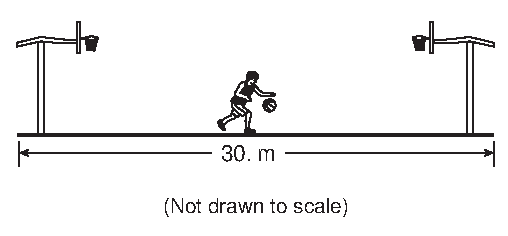
\includegraphics[keepaspectratio,scale=0.75]{June2012-Q01}
    \end{center}
    The magnitude of the player's total displacement after running the drill is:
    \begin{multicols}{2}
    \begin{choices}
      \correctchoice{\SI{0.0}{\meter}}
        \wrongchoice{\SI{30}{\meter}}
        \wrongchoice{\SI{60}{\meter}}
        \wrongchoice{\SI{180}{\meter}}
    \end{choices}
    \end{multicols}
\end{question}
}

\element{nysed}{
\begin{question}{June2012-Q02}
    In a drill during basketball practice,
        a player runs the length of the \SI{30}{\meter} court and back.
    The player does this three times in \SI{60}{\second}.
    \begin{center}
        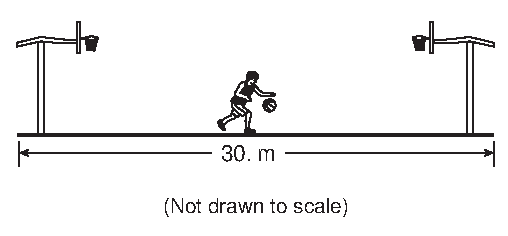
\includegraphics[keepaspectratio,scale=0.75]{June2012-Q01}
    \end{center}
    The average speed of the player during the drill is:
    \begin{multicols}{2}
    \begin{choices}
        \wrongchoice{\SI{0.0}{\meter\per\second}}
        \wrongchoice{\SI{0.50}{\meter\per\second}}
      \correctchoice{\SI{3.0}{\meter\per\second}}
        \wrongchoice{\SI{30}{\meter\per\second}}
    \end{choices}
    \end{multicols}
\end{question}
}


%% Section June2011
%%--------------------


%% Section June2010
%%--------------------
\element{nysed}{
\begin{question}{June2010-Q01}
    A baseball player runs \SI{27.4}{\meter} from the batter's box to first base,
        overruns first base by \SI{3.0}{\meter},
        and then returns to first base.
    Compared to the total distance traveled by the player,
        the magnitude of the player's total displacement from the batter's box is?
    \begin{multicols}{2}
    \begin{choices}
        \wrongchoice{\SI{3.0}{\meter} shorter}
      \correctchoice{\SI{6.0}{\meter} shorter}
        \wrongchoice{\SI{3.0}{\meter} longer}
        \wrongchoice{\SI{6.0}{\meter} longer}
    \end{choices}
    \end{multicols}
\end{question}
}


%% Section June2009
%%--------------------
\element{nysed}{
\begin{question}{June2009-Q01}
    On a highway, a car is driven \SI{80}{\kilo\meter} during the first \SI{1.00}{\hour} of travel,
        \SI{50}{\kilo\meter} during the next \SI{0.50}{\hour},
        and \SI{40}{\kilo\meter} in the final \SI{0.50}{\hour}.
    What is the car's average speed for the entire trip?
    \begin{multicols}{2}
    \begin{choices}
        \wrongchoice{\SI{45}{\kilo\meter\per\hour}}
        \wrongchoice{\SI{60}{\kilo\meter\per\hour}}
      \correctchoice{\SI{85}{\kilo\meter\per\hour}}
        \wrongchoice{\SI{170}{\kilo\meter\per\hour}}
    \end{choices}
    \end{multicols}
\end{question}
}

\element{nysed}{
\begin{question}{June2009-Q04}
    A high-speed train in Japan travels a distance of \SI{300}{\kilo\meter} in \SI{3.60e3}{\second}.
    What is the average speed of this train?
    \begin{multicols}{2}
    \begin{choices}
        \wrongchoice{\SI{1.20e-2}{\meter\per\second}}
        \wrongchoice{\SI{8.33e-2}{\meter\per\second}}
        \wrongchoice{\SI{12.0}{\meter\per\second}}
      \correctchoice{\SI{83.3}{\meter\per\second}}
    \end{choices}
    \end{multicols}
\end{question}
}


%% Section Jan2009
%%--------------------


%% Section June2008
%%--------------------
\element{nysed}{
\begin{question}{June2008-Q04}
    Approximately how much time does it take light to travel from Sun to Earth?
    \begin{multicols}{2}
    \begin{choices}
        \wrongchoice{\SI{2.00e-3}{\second}}
        \wrongchoice{\SI[retain-zero-exponent]{1.28e0}{\second}}
      \correctchoice{\SI{5.00e2}{\second}}
        \wrongchoice{\SI{4.50e19}{\second}}
    \end{choices}
    \end{multicols}
\end{question}
}


%% Section Jan2008
%%--------------------


%% Section June2007
%%--------------------


%% Section Jan2007
%%--------------------


%% Section June2006
%%--------------------


%% Section Jan2006
%%--------------------


%% Section June2005
%%--------------------


%% Section Jan2005
%%--------------------
\element{nysed}{
\begin{question}{Jan2005-Q02}
    In a \SI{4.0}{\kilo\meter} race, a runner completes the first kilometer in \SI{5.9}{\minute},
        the second kilometer in \SI{6.2}{\minute}, and the third kilometer in \SI{6.3}{\minute},
        and the final kilometer in \SI{6.0}{\minute}.
    The average speed of the runner for the race is approximately:
    \begin{multicols}{2}
    \begin{choices}
      \correctchoice{\SI{0.16}{\kilo\meter\per\minute}}
        \wrongchoice{\SI{0.33}{\kilo\meter\per\minute}}
        \wrongchoice{\SI{12}{\kilo\meter\per\minute}}
        \wrongchoice{\SI{24}{\kilo\meter\per\minute}}
    \end{choices}
    \end{multicols}
\end{question}
}


%% Section June2004
%%--------------------


%% Section Jan2004
%%--------------------


%% Section June2003
%%--------------------


%% Section Jan2003
%%--------------------


%% Section Aug2002
%%--------------------


%% Section June2002
%%--------------------


%% Section Jan2002
%%--------------------
\element{nysed}{
\begin{question}{Jan2002-Q03}
    A group of bike riders took a \SI{4.0}{\hour} trip.
    During the first \SI{3.0}{\hour},
        they traveled a total of \SI{50}{\kilo\meter},
        but during the last hour they traveled only \SI{10}{\kilo\meter}.
    What was the group's average speed for the entire trip?
    \begin{multicols}{2}
    \begin{choices}
      \correctchoice{\SI{15}{\kilo\meter\per\hour}}
        \wrongchoice{\SI{30}{\kilo\meter\per\hour}}
        \wrongchoice{\SI{40}{\kilo\meter\per\hour}}
        \wrongchoice{\SI{60}{\kilo\meter\per\hour}}
    \end{choices}
    \end{multicols}
\end{question}
}


%% Section June2001
%%--------------------
\element{nysed}{
\begin{question}{June2001-Q09}
    Two cars, $A$ and $B$, are \SI{400}{\meter} apart.
    Car $A$ travels due east at \SI{30}{\meter\per\second} on a collision course with car $B$,
        which travels due west at \SI{20}{\meter\per\second}.
    How much time elapses before the two cars collide?
    \begin{multicols}{2}
    \begin{choices}
      \correctchoice{\SI{8.0}{\second}}
        \wrongchoice{\SI{20}{\second}}
        \wrongchoice{\SI{13}{\second}}
        \wrongchoice{\SI{40}{\second}}
    \end{choices}
    \end{multicols}
\end{question}
}

\element{nysed}{
\begin{question}{June2001-Q53}
    A softball player leaves the batter's box,
        overruns first base by \SI{3.0}{\meter},
        and then returns to first base.
    Compared to the total distance traveled by the player,
        the magnitude of the player's total displacement from the batter's box is:
    \begin{multicols}{3}
    \begin{choices}
      \correctchoice{smaller}
        \wrongchoice{larger}
        \wrongchoice{the same}
    \end{choices}
    \end{multicols}
\end{question}
}


%% Section Jan2001
%%--------------------


%% Section June2000
%%--------------------


%% Section June1999
%%--------------------


%% Section June1998
%%--------------------
\element{nysed}{
\begin{question}{June1998-Q05}
    What is the average velocity of a car that travels \SI{30}{\kilo\meter} due west in \SI{0.50}{\hour}?
    \begin{multicols}{2}
    \begin{choices}
        \wrongchoice{\SI{15}{\kilo\meter\per\hour}}
        \wrongchoice{\SI{60}{\kilo\meter\per\hour}}
        \wrongchoice{\SI{15}{\kilo\meter\per\hour} west}
      \correctchoice{\SI{60}{\kilo\meter\per\hour} west}
    \end{choices}
    \end{multicols}
\end{question}
}


%% Section June1997
%%--------------------
\element{nysed}{
\begin{question}{June1997-Q02}
    A baseball pitcher throws a fastball at \SI{42}{\meter\per\second}.
    If the batter is \SI{18}{\meter} from the pitcher,
        approximately how much time does it take for the ball to reach the batter?
    \begin{multicols}{2}
    \begin{choices}
        \wrongchoice{\SI{1.0}{\second}}
        \wrongchoice{\SI{2.3}{\second}}
        \wrongchoice{\SI{0.86}{\second}}
      \correctchoice{\SI{0.43}{\second}}
    \end{choices}
    \end{multicols}
\end{question}
}


%% Section June1996
%%--------------------
\element{nysed}{
\begin{question}{June1996-Q01}
    A car travels between the \SI{100}{\meter} and \SI{250}{\meter} highway markers in \SI{10}{\second}.
    The average speed of the car during this interval is:
    \begin{multicols}{2}
    \begin{choices}
        \wrongchoice{\SI{10}{\meter\per\second}}
      \correctchoice{\SI{15}{\meter\per\second}}
        \wrongchoice{\SI{25}{\meter\per\second}}
        \wrongchoice{\SI{35}{\meter\per\second}}
    \end{choices}
    \end{multicols}
\end{question}
}


%% Section June1994
%%--------------------
\element{nysed}{
\begin{question}{June1994-Q44}
    The distance from the Moon to Earth is \SI{3.9e8}{\meter}.
    What is the time required for a light ray to travel from the Moon to Earth?
    \begin{multicols}{2}
    \begin{choices}
        \wrongchoice{\SI{0.65}{\second}}
      \correctchoice{\SI{1.3}{\second}}
        \wrongchoice{\SI{2.6}{\second}}
        \wrongchoice{\SI{3.9}{\second}}
    \end{choices}
    \end{multicols}
\end{question}
}


%% Section June1986
%%--------------------
\element{nysed}{
\begin{question}{June1986-Q02}
    The average speed of a plane was \SI{600}{\kilo\meter\per\hour}.
    How long did it take the plane to travel \SI{120}{\kilo\meter}?
    \begin{multicols}{2}
    \begin{choices}
      \correctchoice{\SI{0.2}{\hour}}
        \wrongchoice{\SI{0.5}{\hour}}
        \wrongchoice{\SI{0.7}{\hour}}
        \wrongchoice{\SI{5}{\hour}}
    \end{choices}
    \end{multicols}
\end{question}
}

\element{nysed}{
\begin{question}{June1986-Q19}
    It takes \SI{1}{\second} for a sound wave to travel from a source to observer $A$.
    How long does it take the same sound wave to travel in the same medium to observer $B$,
        who is located twice as far from the source as observer $A$?
    \begin{multicols}{4}
    \begin{choices}
        \wrongchoice{\SI{1/4}{\second}}
      \correctchoice{\SI{2}{\second}}
        \wrongchoice{\SI{1/2}{\second}}
        \wrongchoice{\SI{4}{\second}}
    \end{choices}
    \end{multicols}
\end{question}
}


%% Section June1985
%%--------------------
\element{nysed}{
\begin{question}{June1985-Q02}
    The distance-time graph below represents the position of an object moving in a straight line.
    \begin{center}
    \begin{tikzpicture}
        \begin{axis}[
            axis y line=left,
            axis x line=bottom,
            axis line style={->},
            xlabel={time},
            x unit=\si{\second},
            xtick={0,1,2,3,4,5,6},
            minor x tick num=1,
            ylabel={distance},
            y unit=\si{\meter},
            ytick={0,10,20,30},
            minor y tick num=1,
            xmin=0,xmax=6.3,
            ymin=0,ymax=31.5,
            width=0.8\columnwidth,
            height=0.5\columnwidth,
            grid=major,
            very thin,
        ]
        \addplot[line width=1pt,mark=\empty] plot coordinates { (0,0) (2,10) (4,30) (6,30)};
        \end{axis}
    \end{tikzpicture}
    \end{center}
    What is the speed of the object during the time interval $t=\SI{2.0}{\second}$ to $t=\SI{4.0}{\second}$?
    \begin{multicols}{2}
    \begin{choices}
        \wrongchoice{\SI{0.0}{\meter\per\second}}
        \wrongchoice{\SI{5.0}{\meter\per\second}}
        \wrongchoice{\SI{7.5}{\meter\per\second}}
      \correctchoice{\SI{10.}{\meter\per\second}}
    \end{choices}
    \end{multicols}
\end{question}
}



\endinput




%% Constant Accleration Questions
%% NYSED Physics Regents Examination
%%--------------------------------------------------

%% this section contains 59 problems


%% Section June2015
%%--------------------
\element{nysed}{
\begin{question}{June2015-Q40}
    A car, initially traveling at \SI{15}{\meter\per\second} north,
        accelerates to \SI{25}{\meter\per\second} north in \SI{4.0}{\second}.
    The magnitude of the average acceleration is:
    \begin{multicols}{2}
    \begin{choices}
      \correctchoice{\SI{2.5}{\meter\per\second\squared}}
        \wrongchoice{\SI{6.3}{\meter\per\second\squared}}
        \wrongchoice{\SI{10.}{\meter\per\second\squared}}
        \wrongchoice{\SI{20.}{\meter\per\second\squared}}
    \end{choices}
    \end{multicols}
\end{question}
}


%% Section June2014
%%--------------------
\element{nysed}{
\begin{question}{June2014-Q02}
    What is the final speed of an object that starts from rest and accelerates uniformly at \SI{4.0}{\meter\per\second\squared} over a distance of \SI{8.0}{\meter}?
    \begin{multicols}{2}
    \begin{choices}
      \correctchoice{\SI{8.0}{\meter\per\second}}
        \wrongchoice{\SI{16}{\meter\per\second}}
        \wrongchoice{\SI{32}{\meter\per\second}}
        \wrongchoice{\SI{64}{\meter\per\second}}
    \end{choices}
    \end{multicols}
\end{question}
}

\element{nysed}{
\begin{question}{June2014-Q07}
    A truck, initially traveling at a speed of \SI{22}{\meter\per\second},
        increases speed at a constant rate of \SI{2.4}{\meter\per\second\squared} for \SI{3.2}{\second}.
    What is the total distance traveled by the truck during this \SI{3.2}{\second} time interval?
    \begin{multicols}{2}
    \begin{choices}
      \correctchoice{\SI{83}{\meter}}
        \wrongchoice{\SI{70.}{\meter}}
        \wrongchoice{\SI{12}{\meter}}
        \wrongchoice{\SI{58}{\meter}}
    \end{choices}
    \end{multicols}
\end{question}
}


%% Section June2013
%%--------------------
\element{nysed}{
\begin{question}{June2013-Q03}
    A car traveling west in a straight line on a highway decreases its speed from \SI{30.0}{\meter\per\second} to \SI{23.0}{\meter\per\second} in \SI{2.00}{\second}.
    The car's average acceleration during this time interval is:
    \begin{multicols}{2}
    \begin{choices}
      \correctchoice{\SI{3.5}{\meter\per\second\squared} east}
        \wrongchoice{\SI{3.5}{\meter\per\second\squared} west}
        \wrongchoice{\SI{13}{\meter\per\second\squared} east}
        \wrongchoice{\SI{13}{\meter\per\second\squared} west}
    \end{choices}
    \end{multicols}
\end{question}
}

\element{nysed}{
\begin{question}{June2013-Q04}
    In a race, a runner traveled \SI{12}{\meter} in \SI{4.0}{\second} as she accelerated uniformly from rest.
    The magnitude of the acceleration of the runner was:
    \begin{multicols}{2}
    \begin{choices}
        \wrongchoice{\SI{0.25}{\meter\per\second\squared}}
      \correctchoice{\SI{1.5}{\meter\per\second\squared}}
        \wrongchoice{\SI{3.0}{\meter\per\second\squared}}
        \wrongchoice{\SI{48}{\meter\per\second\squared}}
    \end{choices}
    \end{multicols}
\end{question}
}


%% Section June2012
%%--------------------
\element{nysed}{
\begin{question}{June2012-Q06}
    A car, initially traveling east with a speed of \SI{5.0}{\meter\per\second},
        is accelerated uniformly at \SI{2.0}{\meter\per\second\squared} east for \SI{10}{\second} along a straight line.
    During this \SI{10}{\second} interval the car travels a total distance of:
    \begin{multicols}{2}
    \begin{choices}
        \wrongchoice{\SI{50}{\meter}}
        \wrongchoice{\SI{60}{\meter}}
        \wrongchoice{\SI{1.0e2}{\meter}}
      \correctchoice{\SI{1.5e2}{\meter}}
    \end{choices}
    \end{multicols}
\end{question}
}

\element{nysed}{
\begin{question}{June2012-Q08}
    A child riding a bicycle at \SI{15}{\meter\per\second} accelerates at \SI{-3.0}{\meter\per\second\squared} for \SI{4.0}{\second}.
    What is the child's speed at the end of this \SI{4.0}{\second} interval?
    \begin{multicols}{2}
    \begin{choices}
        \wrongchoice{\SI{12}{\meter\per\second}}
        \wrongchoice{\SI{27}{\meter\per\second}}
      \correctchoice{\SI{3.0}{\meter\per\second}}
        \wrongchoice{\SI{7.0}{\meter\per\second}}
    \end{choices}
    \end{multicols}
\end{question}
}


%% Section June2011
%%--------------------
\element{nysed}{
\begin{question}{June2011-Q02}
    If a car accelerates uniformly from rest to \SI{15}{\meter\per\second} over a distance of \SI{100}{\meter},
        the magnitude of a car's acceleration is:
    \begin{multicols}{2}
    \begin{choices}
        \wrongchoice{\SI{0.15}{\meter\per\second\squared}}
      \correctchoice{\SI{1.1}{\meter\per\second\squared}}
        \wrongchoice{\SI{2.3}{\meter\per\second\squared}}
        \wrongchoice{\SI{6.7}{\meter\per\second\squared}}
    \end{choices}
    \end{multicols}
\end{question}
}

\element{nysed}{
\begin{question}{June2011-Q03}
    An object accelerates uniformly from \SI{3.0}{\meter\per\second} east to \SI{8.0}{\meter\per\second} east in \SI{2.0}{\second}.
    What is the magnitude of the acceleration of the object?
    \begin{multicols}{2}
    \begin{choices}
      \correctchoice{\SI{2.5}{\meter\per\second\squared}}
        \wrongchoice{\SI{5.0}{\meter\per\second\squared}}
        \wrongchoice{\SI{5.5}{\meter\per\second\squared}}
        \wrongchoice{\SI{11}{\meter\per\second\squared}}
    \end{choices}
    \end{multicols}
\end{question}
}

\element{nysed}{
\begin{question}{June2011-Q04}
    A rock is dropped from a bridge.
    What happens to the magnitude of the acceleration and the speed of the rock as it falls?
    [Neglect friction.]
    \begin{choices}
        \wrongchoice{Both acceleration and speed increase.}
        \wrongchoice{Both acceleration and speed remain the same.}
        \wrongchoice{Acceleration increases and speed decreases.}
      \correctchoice{Acceleration remains the same and speed increases.}
    \end{choices}
\end{question}
}

\element{nysed}{
\begin{question}{June2011-Q05}
    A soccer ball is kicked on a level field has an initial vertical velocity component of \SI{15.0}{\meter\per\second}.
    Assuming the ball lands at the same height from which it was kicked,
        what is the total time the ball is in the air?
    [Neglect friction.]
    \begin{multicols}{2}
    \begin{choices}
        \wrongchoice{\SI{0.654}{\second}}
        \wrongchoice{\SI{1.53}{\second}}
      \correctchoice{\SI{3.06}{\second}}
        \wrongchoice{\SI{6.12}{\second}}
    \end{choices}
    \end{multicols}
\end{question}
}

\element{nysed}{
\begin{question}{June2011-Q37}
    The graph below shows the relationship between the speed and elapsed time for an object falling freely from rest near the surface of a planet.
    \begin{center}
    \begin{tikzpicture}
        \begin{axis}[
            axis y line=left,
            axis x line=bottom,
            axis line style={->},
            xlabel={Time},
            x unit=\si{\second},
            xtick={0.0,1.0,2.0,3.0,4.0},
            ylabel={Speed},
            y unit=\si{\meter\per\second},
            ytick={0.0,2.0,4.0,6.0,8.0,10.0},
            xmin=0,xmax=4,
            ymin=0,ymax=10,
            grid=major,
            width=0.8\columnwidth,
            height=0.5\columnwidth,
            very thin,
        ]
        \addplot[line width=1pt,domain=0:4]{8*x/3};
        \end{axis}
    \end{tikzpicture}
    \end{center}
    What is the total distance the object falls during
        the first \SI{3.0}{\second}?
    \begin{multicols}{2}
    \begin{choices}
      \correctchoice{\SI{12}{\meter}}
        \wrongchoice{\SI{24}{\meter}}
        \wrongchoice{\SI{44}{\meter}}
        \wrongchoice{\SI{72}{\meter}}
    \end{choices}
    \end{multicols}
\end{question}
}


%% Section June2010
%%--------------------
\element{nysed}{
\begin{question}{June2010-Q03}
    A car traveling on a straight road at \SI{15.0}{\meter\per\second} accelerates uniformly to a speed of \SI{21.0}{\meter\per\second} in \SI{12.0}{\second}.
    The total distance traveled by the car in this \SI{12.0}{\second} time interval is:
    \begin{multicols}{2}
    \begin{choices}
        \wrongchoice{\SI{36.0}{\meter}}
        \wrongchoice{\SI{180}{\meter}}
      \correctchoice{\SI{216}{\meter}}
        \wrongchoice{\SI{252}{\meter}}
    \end{choices}
    \end{multicols}
\end{question}
}


%% Section June2009
%%--------------------
\newcommand{\myJuneZeroNineQthirtySevenTikz}{
    \begin{tikzpicture}
        \begin{axis}[
            axis y line=left,
            axis x line=bottom,
            axis line style={->},
            xlabel={time},
            x unit=\si{\second},
            xtick={0,2,4,6},
            ylabel={velocity},
            y unit=\si{\meter\per\second},
            ytick={0,5,10,15},
            xmin=0,xmax=6.5,
            ymin=0,ymax=16,
            grid=major,
            width=0.8\columnwidth,
            height=0.5\columnwidth,
            very thin,
        ]
        \addplot[line width=1pt,domain=0:4]{2.5*x};
        \addplot[line width=1pt,domain=4:6]{10};
        \end{axis}
    \end{tikzpicture}
}

\element{nysed}{
\begin{question}{June2009-Q37}
    The diagram below represents the motion of a car during a \SI{6.0}{\second} time interval.
    \begin{center}
        \myJuneZeroNineQthirtySevenTikz
    \end{center}
    What is the acceleration of the car at $t=\SI{5.0}{\second}$?
    \begin{multicols}{2}
    \begin{choices}
      \correctchoice{\SI{0.0}{\meter\per\second\squared}}
        \wrongchoice{\SI{2.0}{\meter\per\second\squared}}
        \wrongchoice{\SI{2.5}{\meter\per\second\squared}}
        \wrongchoice{\SI{10.0}{\meter\per\second\squared}}
    \end{choices}
    \end{multicols}
\end{question}
}

\element{nysed}{
\begin{question}{June2009-Q38}
    The diagram below represents the motion of a car during a \SI{6.0}{\second} time interval.
    \begin{center}
        \myJuneZeroNineQthirtySevenTikz
    \end{center}
    What is the total distance traveled by the car during this \SI{6.0}{\second} interval?
    \begin{multicols}{2}
    \begin{choices}
        \wrongchoice{\SI{10.}{\meter}}
        \wrongchoice{\SI{20.}{\meter}}
      \correctchoice{\SI{40.}{\meter}}
        \wrongchoice{\SI{60.}{\meter}}
    \end{choices}
    \end{multicols}
\end{question}
}


%% Section Jan2009
%%--------------------
\element{nysed}{
\begin{question}{Jan2009-Q04}
    As a car driven south in a straight line with \emph{decreasing} speed,
        the acceleration of the car must be:
    \begin{choices}
      \correctchoice{directed northward}
        \wrongchoice{directed southward}
        \wrongchoice{zero}
        \wrongchoice{constant, but not zero}
    \end{choices}
\end{question}
}


%% Section June2008
%%--------------------
\element{nysed}{
\begin{question}{June2008-Q07}
    The speed of an object undergoing constant acceleration increases from \SI{8.0}{\meter\per\second} to \SI{16.0}{\meter\per\second} in \SI{10}{\second}.
    How far does the object travel during the \SI{10}{\second}?
    \begin{multicols}{2}
    \begin{choices}
        \wrongchoice{\SI{3.6e2}{\meter}}
        \wrongchoice{\SI{1.6e2}{\meter}}
      \correctchoice{\SI{1.2e2}{\meter}}
        \wrongchoice{\SI{8.0e1}{\meter}}
    \end{choices}
    \end{multicols}
\end{question}
}

\element{nysed}{
\begin{question}{June2008-Q37}
    The graph below represents the displacement of an object moving in a straight line as a function of time.
    \begin{center}
    \begin{tikzpicture}
        \begin{axis}[
            axis y line=left,
            axis x line=bottom,
            axis line style={->},
            xlabel={Time},
            x unit=\si{\second},
            xtick={0.0,2.0,4.0,6.0,8.0,10,0},
            ylabel={displacement},
            y unit=\si{\meter},
            ytick={0,4,8,12,16},
            xmin=0,xmax=10,
            ymin=0,ymax=16,
            grid=major,
            width=0.8\columnwidth,
            height=0.5\columnwidth,
            very thin,
        ]
        \addplot[line width=1pt,domain=0:4]{2*x};
        \addplot[line width=1pt,domain=4:6]{8};
        \addplot[line width=1pt,domain=6:10]{ 8 - 2*( (x-6) * (x-10) )};
        \end{axis}
    \end{tikzpicture}
    \end{center}
    What was the total distance traveled by the object during the \SI{10}{\second} time interval?
    \begin{multicols}{2}
    \begin{choices}
        \wrongchoice{\SI{0}{\meter}}
        \wrongchoice{\SI{8}{\meter}}
        \wrongchoice{\SI{16}{\meter}}
      \correctchoice{\SI{24}{\meter}}
    \end{choices}
    \end{multicols}
\end{question}
}


%% Section Jan2008
%%--------------------
\element{nysed}{
\begin{question}{Jan2008-Q02}
    A race car starting from rest accelerates uniformly at a rate of \SI{4.9}{\meter\per\second\squared}.
    What is the car's speed after it has traveled \SI{200}{\meter}.
    \begin{multicols}{2}
    \begin{choices}
      \correctchoice{\SI{44.3}{\meter\per\second}}
        \wrongchoice{\SI{62.6}{\meter\per\second}}
        \wrongchoice{\SI{1960}{\meter\per\second}}
        \wrongchoice{\SI{31.3}{\meter\per\second}}
    \end{choices}
    \end{multicols}
\end{question}
}


%% Section June2007
%%--------------------
\element{nysed}{
\begin{question}{June2007-Q02}
    An astronaut standing on a platform on the Moon drops a hammer.
    If the hammer falls \SI{6.0}{\meter} vertically in \SI{2.7}{\second},
        what is the acceleration?
    \begin{multicols}{2}
    \begin{choices}
      \correctchoice{\SI{1.6}{\meter\per\second\squared}}
        \wrongchoice{\SI{2.2}{\meter\per\second\squared}}
        \wrongchoice{\SI{4.4}{\meter\per\second\squared}}
        \wrongchoice{\SI{9.8}{\meter\per\second\squared}}
    \end{choices}
    \end{multicols}
\end{question}
}

\element{nysed}{
\begin{question}{June2007-Q40}
    An observer recorded the following data for the motion of a car undergoing constant acceleration.
    \begin{center}
    \begin{tabu}{cc}
        Time (\si{\second}) & Speed (\si{\meter\per\second}) \\
        \midrule
        3.0 & 4.0 \\
        5.0 & 7.0 \\
        6.0 & 8.5 \\
    \end{tabu}
    \end{center}
    What was the magnitude of the acceleration of the car?
    \begin{multicols}{2}
    \begin{choices}
        \wrongchoice{\SI{1.3}{\meter\per\second\squared}}
        \wrongchoice{\SI{2.0}{\meter\per\second\squared}}
      \correctchoice{\SI{1.5}{\meter\per\second\squared}}
        \wrongchoice{\SI{4.5}{\meter\per\second\squared}}
    \end{choices}
    \end{multicols}
\end{question}
}


%% Section Jan2007
%%--------------------
\element{nysed}{
\begin{question}{Jan2007-Q03}
    A car increases its speed from \SI{9.6}{\meter\per\second} to \SI{11.2}{\meter\per\second} in \SI{4.0}{\second}.
    The average acceleration of the car during this \SI{4.0}{\second} interval is:
    \begin{multicols}{2}
    \begin{choices}
      \correctchoice{\SI{0.40}{\meter\per\second\squared}}
        \wrongchoice{\SI{2.4}{\meter\per\second\squared}}
        \wrongchoice{\SI{2.8}{\meter\per\second\squared}}
        \wrongchoice{\SI{5.2}{\meter\per\second\squared}}
    \end{choices}
    \end{multicols}
\end{question}
}

\element{nysed}{
\begin{question}{Jan2007-Q36}
    A cart travels with a constant nonzero acceleration along a straight line.
    Which graph best represents the relationship between the distance the cart travels and the time of travel?
    \begin{multicols}{2}
    \begin{choices}
        \AMCboxDimensions{down=-2.5em}
        \correctchoice{
            \begin{tikzpicture}
                \begin{axis}[
                    axis y line=left,
                    axis x line=bottom,
                    axis line style={->},
                    xlabel={time},
                    xtick=\empty,
                    ylabel={distance},
                    ytick=\empty,
                    xmin=0,xmax=11,
                    ymin=0,ymax=11,
                    width=\columnwidth,
                    very thin,
                ]
                \addplot[line width=1pt,domain=0:10]{0.1 * x*x};
                \end{axis}
            \end{tikzpicture}
        }
        \wrongchoice{
            \begin{tikzpicture}
                \begin{axis}[
                    axis y line=left,
                    axis x line=bottom,
                    axis line style={->},
                    xlabel={time},
                    xtick=\empty,
                    ylabel={distance},
                    ytick=\empty,
                    xmin=0,xmax=11,
                    ymin=0,ymax=11,
                    width=\columnwidth,
                    very thin,
                ]
                \addplot[line width=1pt,domain=0:10]{10-x};
                \end{axis}
            \end{tikzpicture}
        }
        \wrongchoice{
            \begin{tikzpicture}
                \begin{axis}[
                    axis y line=left,
                    axis x line=bottom,
                    axis line style={->},
                    xlabel={time},
                    xtick=\empty,
                    ylabel={distance},
                    ytick=\empty,
                    xmin=0,xmax=185,
                    ymin=0,ymax=10,
                    width=\columnwidth,
                    very thin,
                ]
                \addplot[line width=1pt,domain=0:180]{8*sin(x)};
                \end{axis}
            \end{tikzpicture}
        }
        \wrongchoice{
            \begin{tikzpicture}
                \begin{axis}[
                    axis y line=left,
                    axis x line=bottom,
                    axis line style={->},
                    xlabel={time},
                    xtick=\empty,
                    ylabel={distance},
                    ytick=\empty,
                    xmin=0,xmax=11,
                    ymin=0,ymax=11,
                    width=\columnwidth,
                    very thin,
                ]
                \addplot[line width=1pt,domain=0:10]{x};
                \end{axis}
            \end{tikzpicture}
        }
    \end{choices}
    \end{multicols}
\end{question}
}


%% Section June2006
%%--------------------
\element{nysed}{
\begin{question}{June2006-Q02}
    A rocket initially at rest on the ground lifts off vertically with a constant acceleration of \SI{2.0e1}{\meter\per\second\squared}.
    How long will it take the rocket to reach an altitude of \SI{9.0e3}{\meter}?
    \begin{multicols}{2}
    \begin{choices}
      \correctchoice{\SI{3.0e1}{\second}}
        \wrongchoice{\SI{4.3e1}{\second}}
        \wrongchoice{\SI{4.5e2}{\second}}
        \wrongchoice{\SI{9.0e2}{\second}}
    \end{choices}
    \end{multicols}
\end{question}
}


%% Section Jan2006
%%--------------------
\element{nysed}{
\begin{question}{Jan2006-Q01}
    The speed of a wagon increases from \SI{2.5}{\meter\per\second} to \SI{9.0}{\meter\per\second} in \SI{3.0}{\second} as it accelerates uniformly down a hill.
    what is the magnitude of the acceleration of the wagon during this \SI{3.0}{\second} interval?
    \begin{multicols}{2}
    \begin{choices}
        \wrongchoice{\SI{0.83}{\meter\per\second\squared}}
      \correctchoice{\SI{2.2}{\meter\per\second\squared}}
        \wrongchoice{\SI{3.0}{\meter\per\second\squared}}
        \wrongchoice{\SI{3.8}{\meter\per\second\squared}}
    \end{choices}
    \end{multicols}
\end{question}
}

\element{nysed}{
\begin{question}{Jan2006-Q38}
    The graph below represents the relationship between speed and time for an object moving along a straight line.
    \begin{center}
    \begin{tikzpicture}
        \begin{axis}[
            axis y line=left,
            axis x line=bottom,
            axis line style={->},
            title={Speed vs. Time},
            xlabel={time},
            xtick={0,1,2,3,4,5},
            x unit=\si{\second},
            ylabel={speed},
            y unit=\si{\meter\per\second},
            ytick={0,5,10,15,20,25},
            xmin=0,xmax=5,
            ymin=0,ymax=25,
            grid=major,
            width=0.8\columnwidth,
            height=0.5\columnwidth,
            very thin,
        ]
        \addplot[line width=1pt,domain=0:5]{5*x};
        \end{axis}
    \end{tikzpicture}
    \end{center}
    What is the total distance traveled by the object during the first \SI{4}{\second}?
    \begin{multicols}{2}
    \begin{choices}
        \wrongchoice{\SI{5}{\meter}}
        \wrongchoice{\SI{20}{\meter}}
      \correctchoice{\SI{40}{\meter}}
        \wrongchoice{\SI{80}{\meter}}
    \end{choices}
    \end{multicols}
\end{question}
}


%% Section Jan2005
%%--------------------
\element{nysed}{
\begin{question}{Jan2005-Q36}
    Which pair of graphs represents the same motion of an object?
    \begin{choices}
        \AMCboxDimensions{down=-2.5em}
        \correctchoice{
            \begin{tikzpicture}
                \begin{groupplot}[
                        axis y line=left,
                        axis x line=bottom,
                        axis line style={->},
                        group style={group size=2 by 1},
                        xtick=\empty,
                        ytick=\empty,
                        width=0.5\columnwidth,
                    ]
                    \nextgroupplot[
                        xlabel={time},
                        ylabel={displacement},
                        xmin=0,xmax=11,
                        ymin=0,ymax=11,
                    ] \addplot[line width=1pt,domain=0:10] {0.1*x*x};
                    \nextgroupplot[
                        xlabel={time},
                        ylabel={velocity},
                        xmin=0,xmax=11,
                        ymin=0,ymax=11,
                    ] \addplot[line width=1pt,domain=0:10] {x};
                \end{groupplot}
            \end{tikzpicture}
        }
        \wrongchoice{
            \begin{tikzpicture}
                \begin{groupplot}[
                        axis y line=left,
                        axis x line=middle,
                        axis line style={->},
                        group style={group size=2 by 1},
                        xtick=\empty,
                        ytick=\empty,
                        width=0.5\columnwidth,
                    ]
                    \nextgroupplot[
                        xlabel={time},
                        ylabel={displacement},
                        x label style={anchor=north east},
                        xmin=0,xmax=11,
                        ymin=-5.5,ymax=5.5,
                    ] \addplot[line width=1pt,domain=0:10] {-5+x};
                    \nextgroupplot[
                        xlabel={time},
                        ylabel={velocity},
                        xmin=0,xmax=11,
                        ymin=-5.5,ymax=5.5,
                    ] \addplot[line width=1pt,domain=0:10] {-3};
                \end{groupplot}
            \end{tikzpicture}
        }
        \wrongchoice{
            \begin{tikzpicture}
                \begin{groupplot}[
                        axis y line=left,
                        axis x line=middle,
                        axis line style={->},
                        group style={group size=2 by 1},
                        xtick=\empty,
                        ytick=\empty,
                        width=0.5\columnwidth,
                    ]
                    \nextgroupplot[
                        xlabel={time},
                        ylabel={displacement},
                        xmin=0,xmax=11,
                        ymin=-5.5,ymax=5.5,
                    ] \addplot[line width=1pt,domain=0:10] {5-x};
                    \nextgroupplot[
                        xlabel={time},
                        ylabel={velocity},
                        x label style={anchor=north east},
                        xmin=0,xmax=11,
                        ymin=-5.5,ymax=5.5,
                    ] \addplot[line width=1pt,domain=0:10] {-5+x};
                \end{groupplot}
            \end{tikzpicture}
        }
        \wrongchoice{
            \begin{tikzpicture}
                \begin{groupplot}[
                        axis y line=left,
                        axis x line=bottom,
                        axis line style={->},
                        group style={group size=2 by 1},
                        xtick=\empty,
                        ytick=\empty,
                        width=0.5\columnwidth,
                    ]
                    \nextgroupplot[
                        xlabel={time},
                        ylabel={displacement},
                        xmin=0,xmax=11,
                        ymin=0,ymax=11,
                    ] \addplot[line width=1pt,domain=0:10] {-0.4 *x * (x-10)};
                    \nextgroupplot[
                        xlabel={time},
                        ylabel={velocity},
                        xmin=0,xmax=11,
                        ymin=0,ymax=11,
                    ] \addplot[line width=1pt,domain=0:10] {8};
                \end{groupplot}
            \end{tikzpicture}
        }
    \end{choices}
\end{question}
}



%% Section Jan2004
%%--------------------
\element{nysed}{
\begin{question}{Jan2004-Q03}
    A skater increases her speed uniformly from \SI{2.0}{\meter\per\second}
        to \SI{7.0}{\meter\per\second} over a distance of \SI{12}{\meter}.
    The magnitude of her acceleration as she travels this \SI{12}{\meter} is:
    \begin{multicols}{2}
    \begin{choices}
      \correctchoice{\SI{1.9}{\meter\per\second\squared}}
        \wrongchoice{\SI{2.2}{\meter\per\second\squared}}
        \wrongchoice{\SI{2.4}{\meter\per\second\squared}}
        \wrongchoice{\SI{3.8}{\meter\per\second\squared}}
    \end{choices}
    \end{multicols}
\end{question}
}


%% Section June2003
%%--------------------
\element{nysed}{
\begin{question}{June2003-Q03}
    A car initially traveling at a speed of \SI{16}{\meter\per\second} accelerates uniformly to a speed of \SI{20}{\meter\per\second} over a distance of \SI{36}{\meter}.
    What is the magnitude of the car's acceleration?
    \begin{multicols}{2}
    \begin{choices}
      \correctchoice{\SI{2.0}{\meter\per\second\squared}}
        \wrongchoice{\SI{0.22}{\meter\per\second\squared}}
        \wrongchoice{\SI{9.0}{\meter\per\second\squared}}
        \wrongchoice{\SI{0.11}{\meter\per\second\squared}}
    \end{choices}
    \end{multicols}
\end{question}
}


%% Section Jan2003
%%--------------------

\element{nysed}{
\begin{question}{Jan2003-Q45}
    Which graph best represents the motion of a block accelerating uniformly down an inclined plane?
    \begin{multicols}{2}
    \begin{choices}
        \AMCboxDimensions{down=-2.5em}
        \correctchoice{
            \begin{tikzpicture}
                \begin{axis}[
                    axis y line=left,
                    axis x line=bottom,
                    axis line style={->},
                    xlabel={time},
                    xtick=\empty,
                    ylabel={distance},
                    ytick=\empty,
                    xmin=0,xmax=11,
                    ymin=0,ymax=11,
                    width=\columnwidth,
                    very thin,
                ]
                \addplot[line width=1pt,domain=0:10]{0.1*x*x};
                \end{axis}
            \end{tikzpicture}
        }
        \wrongchoice{
            \begin{tikzpicture}
                \begin{axis}[
                    axis y line=left,
                    axis x line=bottom,
                    axis line style={->},
                    xlabel={time},
                    xtick=\empty,
                    ylabel={distance},
                    ytick=\empty,
                    xmin=0,xmax=11,
                    ymin=0,ymax=11,
                    width=\columnwidth,
                    very thin,
                ]
                \addplot[line width=1pt,domain=0:10]{x};
                \end{axis}
            \end{tikzpicture}
        }
        \wrongchoice{
            \begin{tikzpicture}
                \begin{axis}[
                    axis y line=left,
                    axis x line=bottom,
                    axis line style={->},
                    xlabel={time},
                    xtick=\empty,
                    ylabel={distance},
                    ytick=\empty,
                    xmin=0,xmax=11,
                    ymin=0,ymax=11,
                    width=\columnwidth,
                    very thin,
                ]
                \addplot[line width=1pt,domain=0:10]{7};
                \end{axis}
            \end{tikzpicture}
        }
        \wrongchoice{
            \begin{tikzpicture}
                \begin{axis}[
                    axis y line=left,
                    axis x line=bottom,
                    axis line style={->},
                    xlabel={time},
                    xtick=\empty,
                    ylabel={distance},
                    ytick=\empty,
                    xmin=0,xmax=11,
                    ymin=0,ymax=11,
                    width=\columnwidth,
                    very thin,
                ]
                \addplot[line width=1pt,domain=0:5]{1+1.2*x};
                \addplot[line width=1pt,domain=5:10]{7};
                \end{axis}
            \end{tikzpicture}
        }
    \end{choices}
    \end{multicols}
\end{question}
}


%% Section Aug2002
%%--------------------
\element{nysed}{
\begin{question}{Aug2002-Q02}
    The speed of a car is increased uniformly from \SI{20}{\meter\per\second} to \SI{30}{\meter\per\second} in \SI{4.0}{\second}.
    The magnitude of the car's average acceleration in this \SI{4.0}{\second} interval is:
    \begin{multicols}{2}
    \begin{choices}
        \wrongchoice{\SI{0.40}{\meter\per\second\squared}}
      \correctchoice{\SI{2.5}{\meter\per\second\squared}}
        \wrongchoice{\SI{10}{\meter\per\second\squared}}
        \wrongchoice{\SI{13}{\meter\per\second\squared}}
    \end{choices}
    \end{multicols}
\end{question}
}

\element{nysed}{
\begin{question}{Aug2002-Q03}
    A roller coaster, traveling with an initial speed of \SI{15}{\meter\per\second},
        decelerates uniformly at \SI{-7.0}{\meter\per\second\squared} to a full stop.
    Approximately how far does the roller coaster travel during its deceleration?
    \begin{multicols}{2}
    \begin{choices}
        \wrongchoice{\SI{1.0}{\meter}}
        \wrongchoice{\SI{2.0}{\meter}}
      \correctchoice{\SI{16}{\meter}}
        \wrongchoice{\SI{32}{\meter}}
    \end{choices}
    \end{multicols}
\end{question}
}

\element{nysed}{
\begin{question}{Aug2002-Q39}
    The graph below shows the velocity of a race car moving along a straight line as a function of time.
    \begin{center}
    \begin{tikzpicture}
        \begin{axis}[
            clip=false,
            axis y line=left,
            axis x line=bottom,
            axis line style={->},
            xlabel={time},
            x unit=\si{\second},
            xtick={0,1,2,3,4},
            ylabel={velocity},
            y unit=\si{\meter\per\second},
            ytick={0,10,20,30,40},
            xmin=0,xmax=4.1,
            ymin=0,ymax=42,
            grid=major,
            width=0.8\columnwidth,
            height=0.5\columnwidth,
            very thin,
        ]
        \addplot[line width=1pt,domain=0:4]{10*x};
        \end{axis}
    \end{tikzpicture}
    \end{center}
    What is the magnitude of the displacement of the car from $t=\SI{2.0}{\second}$ to $t=\SI{4.0}{\second}$?
    \begin{multicols}{2}
    \begin{choices}
        \wrongchoice{\SI{20}{\meter}}
        \wrongchoice{\SI{40}{\meter}}
      \correctchoice{\SI{60}{\meter}}
        \wrongchoice{\SI{80}{\meter}}
    \end{choices}
    \end{multicols}
\end{question}
}


%% Section June2002
%%--------------------
\element{nysed}{
\begin{question}{June2002-Q03}
    An object with an initial speed of \SI{4.0}{\meter\per\second} accelerates uniformly at \SI{2.0}{\meter\per\second\squared} in the direction of its motion for a distance of \SI{5.0}{\meter}.
    What is the final speed of the object?
    \begin{multicols}{2}
    \begin{choices}
      \correctchoice{\SI{6.0}{\meter\per\second}}
        \wrongchoice{\SI{10}{\meter\per\second}}
        \wrongchoice{\SI{14}{\meter\per\second}}
        \wrongchoice{\SI{36}{\meter\per\second}}
    \end{choices}
    \end{multicols}
\end{question}
}

\element{nysed}{
\begin{question}{June2002-Q04}
    After a model rocket reached its maximum height, it then took \SI{5.0}{\second} to return to the launch site.
    What is the approximate maximum height reached by the rocket?
    [Neglect air resistance]
    \begin{multicols}{2}
    \begin{choices}
        \wrongchoice{\SI{49}{\meter}}
        \wrongchoice{\SI{98}{\meter}}
      \correctchoice{\SI{120}{\meter}}
        \wrongchoice{\SI{250}{\meter}}
    \end{choices}
    \end{multicols}
\end{question}
}

\element{nysed}{
\begin{question}{June2002-Q36}
    The displacement-time graph below represents the motion of a cart initially moving in a straight line.
    \begin{center}
    \begin{tikzpicture}
        \begin{axis}[
            clip=false,
            axis y line=left,
            axis x line=bottom,
            axis line style={->},
            xlabel={time},
            xtick=\empty,
            ylabel={displacement},
            ytick=\empty,
            xmin=0,xmax=26,
            ymin=0,ymax=12,
            width=0.8\columnwidth,
            height=0.5\columnwidth,
            very thin,
        ]
        \addplot[line width=1pt,domain=0:5]{0.24*x*x}
            node[black,pos=0,anchor=north] {$A$};
        \addplot[line width=1pt,domain=5:14]{6 + (x-5)/3}
            node[black,pos=0,anchor=south] {$B$};
        \addplot[line width=1pt,domain=14:20]{9}
            node[black,pos=0,anchor=south] {$C$};
        \addplot[line width=1pt,domain=20:24]{9 - 1.25*(x-20)}
            node[black,pos=0,anchor=south west] {$D$}
            node[black,pos=1,anchor=west] {$E$};
        \addplot[only marks,mark=*,mark size=2pt] coordinates
            { (0,0) (5,6) (14,9) (20,9) (24,4) };
        \end{axis}
    \end{tikzpicture}
    \end{center}
    During which interval is the cart moving forward at constant speed?
    \begin{multicols}{2}
    \begin{choices}
        \wrongchoice{$AB$}
      \correctchoice{$BC$}
        \wrongchoice{$CD$}
        \wrongchoice{$DE$}
    \end{choices}
    \end{multicols}
\end{question}
}


%% Section Jan2002
%%--------------------
\element{nysed}{
\begin{question}{Jan2002-Q04}
    A skier starting from rest skis straight down a slope \SI{50}{\meter} long in \SI{5.0}{\second}.
    What is the magnitude of the acceleration of the skier?
    \begin{multicols}{2}
    \begin{choices}
        \wrongchoice{\SI{20}{\meter\per\second\squared}}
        \wrongchoice{\SI{9.8}{\meter\per\second\squared}}
        \wrongchoice{\SI{5.0}{\meter\per\second\squared}}
      \correctchoice{\SI{4.0}{\meter\per\second\squared}}
    \end{choices}
    \end{multicols}
\end{question}
}


%% Section June2001
%%--------------------
\element{nysed}{
\begin{question}{June2001-Q03}
    Which graph best represents the motion of an object whose speed is increasing?
    \begin{multicols}{2}
    \begin{choices}
        \AMCboxDimensions{down=-2.5em}
        \correctchoice{
            \begin{tikzpicture}
                \begin{axis}[
                    axis y line=left,
                    axis x line=bottom,
                    axis line style={->},
                    xlabel={time},
                    xtick=\empty,
                    ylabel={distance},
                    ytick=\empty,
                    xmin=0,xmax=11,
                    ymin=0,ymax=11,
                    width=\columnwidth,
                    very thin,
                ]
                \addplot[line width=1pt,domain=0:10]{0.1*x*x};
                \end{axis}
            \end{tikzpicture}
        }
        \wrongchoice{
            \begin{tikzpicture}
                \begin{axis}[
                    axis y line=left,
                    axis x line=bottom,
                    axis line style={->},
                    xlabel={time},
                    xtick=\empty,
                    ylabel={distance},
                    ytick=\empty,
                    xmin=0,xmax=11,
                    ymin=0,ymax=11,
                    width=\columnwidth,
                    very thin,
                ]
                \addplot[line width=1pt,domain=0:10]{x};
                \end{axis}
            \end{tikzpicture}
        }
        \wrongchoice{
            \begin{tikzpicture}
                \begin{axis}[
                    axis y line=left,
                    axis x line=bottom,
                    axis line style={->},
                    xlabel={time},
                    xtick=\empty,
                    ylabel={distance},
                    ytick=\empty,
                    xmin=0,xmax=11,
                    ymin=0,ymax=11,
                    width=\columnwidth,
                    very thin,
                ]
                \addplot[line width=1pt,domain=0:10]{10-x};
                \end{axis}
            \end{tikzpicture}
        }
        \wrongchoice{
            \begin{tikzpicture}
                \begin{axis}[
                    axis y line=left,
                    axis x line=bottom,
                    axis line style={->},
                    xlabel={time},
                    xtick=\empty,
                    ylabel={distance},
                    ytick=\empty,
                    xmin=0,xmax=11,
                    ymin=0,ymax=11,
                    width=\columnwidth,
                    very thin,
                ]
                \addplot[line width=1pt,domain=0:10]{10/x};
                \end{axis}
            \end{tikzpicture}
        }
    \end{choices}
    \end{multicols}
\end{question}
}

\element{nysed}{
\begin{question}{June2001-Q05}
    A car having an initial velocity of \SI{12}{\meter\per\second} east slows uniformly to \SI{2}{\meter\per\second} east in \SI{4.0}{\second}.
    The acceleration of the car during this \SI{4.0}{\second} interval is:
    \begin{multicols}{2}
    \begin{choices}
      \correctchoice{\SI{2.5}{\meter\per\second\squared} west}
        \wrongchoice{\SI{2.5}{\meter\per\second\squared} east}
        \wrongchoice{\SI{6.0}{\meter\per\second\squared} west}
        \wrongchoice{\SI{6.0}{\meter\per\second\squared} east}
    \end{choices}
    \end{multicols}
\end{question}
}

\element{nysed}{
\begin{question}{June2001-Q14}
    An airplane originally at rest on a runway accelerates uniformly at \SI{6.0}{\meter\per\second\squared} for \SI{12}{\second}.
    During this \SI{12}{\second} interval,
        the airplane travels a distance of approximately:
    \begin{multicols}{2}
    \begin{choices}
        \wrongchoice{\SI{72}{\meter}}
        \wrongchoice{\SI{220}{\meter}}
      \correctchoice{\SI{430}{\meter}}
        \wrongchoice{\SI{860}{\meter}}
    \end{choices}
    \end{multicols}
\end{question}
}


%% Section Jan2001
%%--------------------
\element{nysed}{
\begin{question}{Jan2001-Q02}
    The diagram below represents the relationship between velocity and time for four cars,
        $A$, $B$, $C$, and $D$, in straight-line motion.
    \begin{center}
    \begin{tikzpicture}
        \begin{axis}[
            axis y line=left,
            axis x line=bottom,
            axis line style={->},
            xlabel={time},
            x unit=\si{\second},
            xtick={0,5,10,15,20},
            ylabel={velocity},
            ytick=\empty,
            xmin=0,xmax=21,
            ymin=0,ymax=10,
            width=0.98\columnwidth,
            height=0.618\columnwidth,
            very thin,
        ]
        \addplot[line width=0.7pt,domain=0:20]{8}
            node[pos=0.1,anchor=south east] {$A$};
        \addplot[line width=1pt,domain=0:20]{4 + 4*x/15}
            node[pos=0.1,anchor=south east] {$B$};
        \addplot[line width=1.25pt,domain=0:20]{8*x/15}
            node[pos=0.1,anchor=south east] {$C$};
        \addplot[line width=1.5pt,domain=10:20]{8*(x-10)/5}
            node[pos=0.0,anchor=south east] {$D$};
        \end{axis}
    \end{tikzpicture}
    \end{center}
    Which car has the greatest acceleration during the time interval \SI{10}{\second} to \SI{15}{\second}?
    \begin{multicols}{4}
    \begin{choices}[o]
        \wrongchoice{$A$}
        \wrongchoice{$B$}
        \wrongchoice{$C$}
      \correctchoice{$D$}
    \end{choices}
    \end{multicols}
\end{question}
}

\element{nysed}{
\begin{question}{Jan2001-Q14}
    %% NOTE: Reword
    %The graph below represents the displacment ($x$)
    %    of an object with respect to time ($t$).
    The graph below represents the motion of an object.
    \begin{center}
    \begin{tikzpicture}
        \begin{axis}[
            axis y line=left,
            axis x line=bottom,
            axis line style={->},
            xlabel={time},
            xtick=\empty,
            ylabel={displacement},
            ytick=\empty,
            xmin=0,xmax=10,
            ymin=0,ymax=10,
            width=0.8\columnwidth,
            height=0.5\columnwidth,
            very thin,
        ]
        \addplot[line width=1pt,domain=0:10]{x};
        \end{axis}
    \end{tikzpicture}
    \end{center}
    According the the graph, as time increases,
        the velocity of the object:
    \begin{choices}
        \wrongchoice{decreases}
        \wrongchoice{increases}
      \correctchoice{remains the same}
    \end{choices}
\end{question}
}


%% Section June2000
%%--------------------
\element{nysed}{
\begin{question}{June2000-Q02}
    Which pair of graphs represents the same motion?
    \begin{choices}
        \AMCboxDimensions{down=-2.5em}
        \correctchoice{
            \begin{tikzpicture}
                \begin{groupplot}[
                        axis y line=left,
                        axis x line=bottom,
                        axis line style={->},
                        group style={group size=2 by 1},
                        xtick=\empty,
                        ytick=\empty,
                        width=0.5\columnwidth,
                    ]
                    \nextgroupplot[
                        xlabel={time},
                        ylabel={displacement},
                        xmin=0,xmax=11,
                        ymin=0,ymax=11,
                    ] \addplot[line width=1pt,domain=0:10] {x};
                    \nextgroupplot[
                        xlabel={time},
                        ylabel={velocity},
                        xmin=0,xmax=11,
                        ymin=0,ymax=11,
                    ] \addplot[line width=1pt,domain=0:10] {5};
                \end{groupplot}
            \end{tikzpicture}
        }
        \wrongchoice{
            \begin{tikzpicture}
                \begin{groupplot}[
                        axis y line=left,
                        axis x line=bottom,
                        axis line style={->},
                        group style={group size=2 by 1},
                        xtick=\empty,
                        ytick=\empty,
                        width=0.5\columnwidth,
                    ]
                    \nextgroupplot[
                        xlabel={time},
                        ylabel={displacement},
                        xmin=0,xmax=11,
                        ymin=0,ymax=11,
                    ] \addplot[line width=1pt,domain=0:10] {5};
                    \nextgroupplot[
                        xlabel={time},
                        ylabel={velocity},
                        xmin=0,xmax=11,
                        ymin=0,ymax=11,
                    ] \addplot[line width=1pt,domain=0:10] {x};
                \end{groupplot}
            \end{tikzpicture}
        }
        \wrongchoice{
            \begin{tikzpicture}
                \begin{groupplot}[
                        axis y line=left,
                        axis x line=bottom,
                        axis line style={->},
                        group style={group size=2 by 1},
                        xtick=\empty,
                        ytick=\empty,
                        width=0.5\columnwidth,
                    ]
                    \nextgroupplot[
                        xlabel={time},
                        ylabel={displacement},
                        xmin=0,xmax=11,
                        ymin=0,ymax=11,
                    ] \addplot[line width=1pt,domain=0:10] {10-x};
                    \nextgroupplot[
                        xlabel={time},
                        ylabel={velocity},
                        xmin=0,xmax=11,
                        ymin=0,ymax=11,
                    ] \addplot[line width=1pt,domain=0:10] {x};
                \end{groupplot}
            \end{tikzpicture}
        }
        \wrongchoice{
            \begin{tikzpicture}
                \begin{groupplot}[
                        axis y line=left,
                        axis x line=bottom,
                        axis line style={->},
                        group style={group size=2 by 1},
                        xtick=\empty,
                        ytick=\empty,
                        width=0.5\columnwidth,
                    ]
                    \nextgroupplot[
                        xlabel={time},
                        ylabel={displacement},
                        xmin=0,xmax=11,
                        ymin=0,ymax=11,
                    ] \addplot[line width=1pt,domain=0:10] {x};
                    \nextgroupplot[
                        xlabel={time},
                        ylabel={velocity},
                        xmin=0,xmax=11,
                        ymin=0,ymax=11,
                    ] \addplot[line width=1pt,domain=0:10] {x};
                \end{groupplot}
            \end{tikzpicture}
        }
    \end{choices}
\end{question}
}

\element{nysed}{
\begin{question}{June2000-Q03}
    A runner starts from rest and accelerates uniformly to a speed of \SI{8.0}{\meter\per\second} in \SI{4.0}{\second}.
    The magnitude of the acceleration of the runner is:
    \begin{multicols}{2}
    \begin{choices}
        \wrongchoice{\SI{0.50}{\meter\per\second\squared}}
      \correctchoice{\SI{2.0}{\meter\per\second\squared}}
        \wrongchoice{\SI{9.8}{\meter\per\second\squared}}
        \wrongchoice{\SI{32}{\meter\per\second\squared}}
    \end{choices}
    \end{multicols}
\end{question}
}


%% Section June1999
%%--------------------
\element{nysed}{
\begin{question}{June1999-Q02}
    A truck with an initial speed of \SI{12}{\meter\per\second} accelerates uniformly at \SI{2.0}{\meter\per\second\squared} for \SI{3.0}{\second}.
    What is the total distance traveled by the truck during this \SI{3.0}{\second} interval?
    \begin{multicols}{2}
    \begin{choices}
        \wrongchoice{\SI{9.0}{\meter}}
        \wrongchoice{\SI{25}{\meter}}
        \wrongchoice{\SI{36}{\meter}}
      \correctchoice{\SI{45}{\meter}}
    \end{choices}
    \end{multicols}
\end{question}
}

\element{nysed}{
\begin{question}{June1999-Q05}
    The graph below represents the relationship between the displacement of an object and its time of travel along a straight line.
    \begin{center}
    \begin{tikzpicture}
        \begin{axis}[
            axis line style={->},
            axis y line=left,
            axis x line=bottom,
            label={displacement vs. time},
            xlabel={time},
            x unit=\si{\second},
            xtick={0,1,2,3,4,5,6,7,8},
            ylabel={displacement},
            y unit=\si{\meter},
            ytick={0,2,4,6,8,10},
            xmin=0,xmax=8.1,
            ymin=0,ymax=10.1,
            grid=major,
            width=0.8\columnwidth,
            height=0.5\columnwidth,
            very thin,
        ]
        \addplot[line width=1pt,domain=0:2]{4*x};
        \addplot[line width=1pt,domain=2:4]{8};
        \addplot[line width=1pt,domain=4:8]{16-2*x};
        \end{axis}
    \end{tikzpicture}
    \end{center}
    What is the magnitude of the object's total displacement after \SI{8.0}{\second}?
    \begin{multicols}{2}
    \begin{choices}
      \correctchoice{\SI{0}{\meter}}
        \wrongchoice{\SI{2}{\meter}}
        \wrongchoice{\SI{8}{\meter}}
        \wrongchoice{\SI{16}{\meter}}
    \end{choices}
    \end{multicols}
\end{question}
}

\element{nysed}{
\begin{question}{June1999-Q06}
    The graph below represents the relationship between the displacement of an object and its time of travel along a straight line.
    \begin{center}
    \begin{tikzpicture}
        \begin{axis}[
            axis line style={->},
            label={displacement vs. time},
            xlabel={time},
            x unit=\si{\second},
            xtick={0,1,2,3,4,5,6,7,8},
            ylabel={displacement},
            y unit=\si{\meter},
            ytick={0,2,4,6,8,10},
            xmin=0,xmax=8,
            ymin=0,ymax=10,
            grid=major,
            width=0.8\columnwidth,
            height=0.5\columnwidth,
            very thin,
        ]
        \addplot[line width=1pt,domain=0:2]{4*x};
        \addplot[line width=1pt,domain=2:4]{8};
        \addplot[line width=1pt,domain=4:8]{16-2*x};
        \end{axis}
    \end{tikzpicture}
    \end{center}
    What is the average speed of the object during the first \SI{4.0}{\second}?
    \begin{multicols}{2}
    \begin{choices}
        \wrongchoice{\SI{0}{\meter\per\second}}
      \correctchoice{\SI{2}{\meter\per\second}}
        \wrongchoice{\SI{8}{\meter\per\second}}
        \wrongchoice{\SI{4}{\meter\per\second}}
    \end{choices}
    \end{multicols}
\end{question}
}

%% Section June1998
%%--------------------
\element{nysed}{
\begin{question}{June1998-Q07}
    A car having an initial speed of \SI{16}{\meter\per\second} is uniformly brought to rest in \SI{4.0}{\second}.
    How far does the car travel during this \SI{4.0}{\second} interval?
    \begin{multicols}{2}
    \begin{choices}
      \correctchoice{\SI{32}{\meter}}
        \wrongchoice{\SI{82}{\meter}}
        \wrongchoice{\SI{96}{\meter}}
        \wrongchoice{\SI{4.0}{\meter}}
    \end{choices}
    \end{multicols}
\end{question}
}


%% Section June1997
%%--------------------
\element{nysed}{
\begin{question}{June1997-Q06}
    The displacement-time graph below represents the motion of a cart along a straight line.
    \begin{center}
    \begin{tikzpicture}
        \begin{axis}[
            clip=false,
            axis y line=left,
            axis x line=bottom,
            axis line style={->},
            xlabel={time},
            xtick=\empty,
            ylabel={displacement},
            ytick=\empty,
            xmin=0,xmax=26,
            ymin=0,ymax=12,
            width=0.8\columnwidth,
            height=0.5\columnwidth,
            very thin,
        ]
        \addplot[line width=1pt,domain=0:5]{0.24*x*x}
            node[black,pos=0,anchor=north west] {$A$};
        \addplot[line width=1pt,domain=5:14]{6 + (x-5)/3}
            node[black,pos=0,anchor=south] {$B$};
        \addplot[line width=1pt,domain=14:20]{9}
            node[black,pos=0,anchor=south] {$C$};
        \addplot[line width=1pt,domain=20:24]{9 - 1.25*(x-20)}
            node[black,pos=0,anchor=south west] {$D$}
            node[black,pos=1,anchor=west] {$E$};
        \addplot[only marks,mark=*,mark size=2pt] coordinates
            { (0,0) (5,6) (14,9) (20,9) (24,4) };
        \end{axis}
    \end{tikzpicture}
    \end{center}
    During which interval was the cart accelerating?
    \begin{multicols}{2}
    \begin{choices}
      \correctchoice{$AB$}
        \wrongchoice{$BC$}
        \wrongchoice{$CD$}
        \wrongchoice{$DE$}
    \end{choices}
    \end{multicols}
\end{question}
}

\element{nysed}{
\begin{question}{June1997-Q09}
    A \SI{1000}{\kilo\gram} car traveling with a velocity of \SI[retain-explicit-plus]{+20}{\meter\per\second} decelerates at \SI{-5.0}{\meter\per\second\squared} until it comes to rest.
    What is the total distance the car travels as it decelerates to rest?
    \begin{multicols}{2}
    \begin{choices}
        \wrongchoice{\SI{10}{\meter}}
        \wrongchoice{\SI{20}{\meter}}
      \correctchoice{\SI{40}{\meter}}
        \wrongchoice{\SI{80}{\meter}}
    \end{choices}
    \end{multicols}
\end{question}
}

\element{nysed}{
\begin{question}{June1997-Q54}
    A bicyclist accelerates from rest to a speed of \SI{5.0}{\meter\per\second} in \SI{10}{\second}.
    During the same \SI{10}{\second},
        a car accelerates from a speed of \SI{22}{\meter\per\second} to a speed of \SI{27}{\meter\per\second}.
    Compared to the acceleration of the bicycle,
        the acceleration of the car is:
    %% NOTE: bike=0.5 m/s/s, car=0.5 m/s/s
    \begin{multicols}{3}
    \begin{choices}
        \wrongchoice{less}
        \wrongchoice{greater}
      \correctchoice{the same}
    \end{choices}
    \end{multicols}
\end{question}
}


%% Section June1996
%%--------------------
\element{nysed}{
\begin{question}{June1996-Q03}
    The graph below represents the relationship between speed and time for a car moving in a straight line.
    \begin{center}
    \begin{tikzpicture}
        \begin{axis}[
            axis y line=left,
            axis x line=bottom,
            axis line style={->},
            xlabel={Time},
            x unit=\si{\second},
            xtick={0.0,1.0,2.0,3.0},
            ylabel={Speed},
            y unit=\si{\meter\per\second},
            ytick={0,10,20,30},
            xmin=0,xmax=3,
            ymin=0,ymax=30,
            grid=major,
            width=0.8\columnwidth,
            height=0.5\columnwidth,
            very thin,
        ]
        \addplot[line width=1pt,domain=0:4]{10*x};
        \end{axis}
    \end{tikzpicture}
    \end{center}
    The magnitude of the car's acceleration is:
    \begin{multicols}{2}
    \begin{choices}
      \correctchoice{\SI{1.0}{\meter\per\second\squared}}
        \wrongchoice{\SI{0.10}{\meter\per\second\squared}}
        \wrongchoice{\SI{10}{\meter\per\second\squared}}
        \wrongchoice{\SI{0.0}{\meter\per\second\squared}}
    \end{choices}
    \end{multicols}
\end{question}
}

\element{nysed}{
\begin{question}{June1996-Q04}
    Oil drips at \SI{0.4}{\second} intervals from a car that has an oil leak.
    Which pattern best represents the spacing of oil drops as the car accelerates uniformly from rest?
    \begin{choices}
        \AMCboxDimensions{down=-0.5em}
        \wrongchoice{
            \begin{tikzpicture}
                \draw[dashed,white!80!black] (-0.2,-1em) rectangle (6.2,1em);
                \foreach \x in {0,15,...,60} \fill (\x mm,0) circle (2pt);
            \end{tikzpicture}
        }
        \correctchoice{
            \begin{tikzpicture}
                \draw[dashed,white!80!black] (-0.2,-1em) rectangle (6.2,1em);
                \foreach \x in {0,1,...,4} \fill ({0.375*\x*\x},0) circle (2pt);
            \end{tikzpicture}
        }
        \wrongchoice{
            \begin{tikzpicture}
                \draw[dashed,white!80!black] (-0.2,-1em) rectangle (6.2,1em);
                \foreach \x in {0,10,20} \fill (\x mm,0) circle (2pt);
                \foreach \x in {40,60} \fill (\x mm,0) circle (2pt);
            \end{tikzpicture}
        }
        \wrongchoice{
            \begin{tikzpicture}
                \draw[dashed,white!80!black] (-0.2,-1em) rectangle (6.2,1em);
                \foreach \x in {0,1,...,5} \fill ({6*rnd},0) circle (2pt);
            \end{tikzpicture}
        }
    \end{choices}
\end{question}
}

\element{nysed}{
\begin{question}{June1996-Q05}
    In an experiment that measures how fast a student reacts,
        a meter stick dropped from rest falls \SI{0.20}{\meter} before the student catches it.
    The reaction time of the student is approximately:
    \begin{multicols}{2}
    \begin{choices}
        \wrongchoice{\SI{0.10}{\second}}
      \correctchoice{\SI{0.20}{\second}}
        \wrongchoice{\SI{0.30}{\second}}
        \wrongchoice{\SI{0.40}{\second}}
    \end{choices}
    \end{multicols}
\end{question}
}

\element{nysed}{
\begin{question}{June1996-Q06}
    A race car traveling \SI{10}{\meter\per\second} accelerates at the rate of \SI{1.5}{\meter\per\second\squared} while traveling a distance of \SI{600}{\meter}.
    The final speed of the race car is approximately:
    \begin{multicols}{2}
    \begin{choices}
        \wrongchoice{\SI{1900}{\meter\per\second}}
        \wrongchoice{\SI{910}{\meter\per\second}}
        \wrongchoice{\SI{150}{\meter\per\second}}
      \correctchoice{\SI{44}{\meter\per\second}}
    \end{choices}
    \end{multicols}
\end{question}
}


%% Section June1994
%%--------------------



%% Section June1990
%%--------------------
\element{nysed}{
\begin{question}{June1990-Q01}
    A cart starting from rest travels a distance of \SI{3.6}{\meter} in \SI{1.8}{\second}.
    The average speed of the cart is:
    \begin{multicols}{2}
    \begin{choices}
        \wrongchoice{\SI{0.20}{\meter\per\second}}
      \correctchoice{\SI{2.0}{\meter\per\second}}
        \wrongchoice{\SI{0.50}{\meter\per\second}}
        \wrongchoice{\SI{5.0}{\meter\per\second}}
    \end{choices}
    \end{multicols}
\end{question}
}

\element{nysed}{
\begin{question}{June1990-Q02}
    An object has a constant acceleration of \SI{2.0}{\meter\per\second\squared}.
    The time required for the object to accelerate from \SI{8.0}{\meter\per\second} to \SI{28}{\meter\per\second} is:
    \begin{multicols}{2}
    \begin{choices}
        \wrongchoice{\SI{20}{\second}}
        \wrongchoice{\SI{16}{\second}}
      \correctchoice{\SI{10}{\second}}
        \wrongchoice{\SI{4.0}{\second}}
    \end{choices}
    \end{multicols}
\end{question}
}

\element{nysed}{
\begin{question}{June1990-Q04}
    A car moving at a speed of \SI{8.0}{\meter\per\second} enters a highway and accelerates at \SI{3.0}{\meter\per\second\squared}.
    How fast will the car be moving after it has accelerated for \SI{56}{\meter}?
    \begin{multicols}{2}
    \begin{choices}
        \wrongchoice{\SI{24}{\meter\per\second}}
      \correctchoice{\SI{20}{\meter\per\second}}
        \wrongchoice{\SI{18}{\meter\per\second}}
        \wrongchoice{\SI{4.0}{\meter\per\second}}
    \end{choices}
    \end{multicols}
\end{question}
}

\element{nysed}{
\begin{question}{June1990-Q06}
    The graph at the right represents the relationship between distance and time for an object in motion.
    \begin{center}
    \begin{tikzpicture}
        \begin{axis}[
            axis y line=left,
            axis x line=bottom,
            axis line style={->},
            xlabel={time},
            xtick=\empty,
            ylabel={distance},
            ytick=\empty,
            xmin=0,xmax=11,
            ymin=0,ymax=11,
            width=0.8\columnwidth,
            height=0.5\columnwidth,
            clip=false,
            very thin,
        ]
        \draw[very thick] (axis cs:0,0) -- (axis cs:2,0) -- (axis cs:4,4) -- (axis cs:7,4) to[out=0,in=220] (axis cs:10,8);
        %% labels
        \node[anchor=north west] at (axis cs:0,0) {$A$};
        \node[anchor=north] at (axis cs:2,0) {$B$};
        \node[anchor=south] at (axis cs:4,4) {$C$};
        \node[anchor=south] at (axis cs:7,4) {$D$};
        \node[anchor=south] at (axis cs:10,8) {$E$};
        \end{axis}
    \end{tikzpicture}
    \end{center}
    During which interval is the speed of the object changing?
    \begin{multicols}{2}
    \begin{choices}
        \wrongchoice{$AB$}
        \wrongchoice{$BC$}
        \wrongchoice{$CD$}
      \correctchoice{$DE$}
    \end{choices}
    \end{multicols}
\end{question}
}


%% Section June1989
%%--------------------
\element{nysed}{
\begin{question}{June1989-Q06}
    If an object's velocity changes from \SI{25}{\meter\per\second} to \SI{15}{\meter\per\second} in \SI{2.0}{\second},
        the magnitude of the object's acceleration Is:
    \begin{multicols}{2}
    \begin{choices}
      \correctchoice{\SI{5.0}{\meter\per\second\squared}}
        \wrongchoice{\SI{7.5}{\meter\per\second\squared}}
        \wrongchoice{\SI{13}{\meter\per\second\squared}}
        \wrongchoice{\SI{20}{\meter\per\second\squared}}
    \end{choices}
    \end{multicols}
\end{question}
}

\element{nysed}{
\begin{question}{June1989-Q07}
    An object initially traveling in a straight line with a speed of \SI{5.0}{\meter\per\second} is accelerated at \SI{2.0}{\meter\per\second\squared} for \SI{4.0}{\second}.
    The total distance traveled by the object in the \SI{4.0}{\second} is:
    \begin{multicols}{2}
    \begin{choices}
      \correctchoice{\SI{36}{\meter}}
        \wrongchoice{\SI{24}{\meter}}
        \wrongchoice{\SI{16}{\meter}}
        \wrongchoice{\SI{4.0}{\meter}}
    \end{choices}
    \end{multicols}
\end{question}
}


%% Section June1986
%%--------------------
\element{nysed}{
\begin{question}{June1986-Q01}
    The graph below represents the motion of a body that is moving with:
    \begin{center}
    \begin{tikzpicture}
        \begin{axis}[
            axis y line=left,
            axis x line=bottom,
            axis line style={->},
            xlabel={time},
            xtick=\empty,
            ylabel={distance},
            ytick=\empty,
            xmin=0,xmax=11,
            ymin=0,ymax=11,
            width=0.8\columnwidth,
            height=0.5\columnwidth,
            very thin,
        ]
        \addplot[line width=1pt,domain=0:10]{x};
        \end{axis}
    \end{tikzpicture}
    \end{center}
    \begin{choices}
        \wrongchoice{increasing acceleration}
        \wrongchoice{decreasing acceleration}
        \wrongchoice{increasing speed}
      \correctchoice{constant speed}
    \end{choices}
\end{question}
}

\element{nysed}{
\begin{question}{June1986-Q03}
    An object initially at rest accelerates at \SI{5}{\meter\per\second\squared} until it attains a speed of \SI{30}{\meter\per\second}.
    What distance does the object move while accelerating?
    \begin{multicols}{2}
    \begin{choices}
        \wrongchoice{\SI{30}{\meter}}
      \correctchoice{\SI{90}{\meter}}
        \wrongchoice{\SI{3}{\meter}}
        \wrongchoice{\SI{600}{\meter}}
    \end{choices}
    \end{multicols}
\end{question}
}

\newcommand{\nysedJuneNineteenEightySixQSixtyOne}{
\begin{tikzpicture}
    \begin{axis}[
        axis y line=left,
        axis x line=bottom,
        axis line style={->},
        xlabel={time},
        x unit=\si{\second},
        xtick={0,1,2,3,4,5,6},
        ylabel={displacement},
        y unit=\si{\meter},
        ytick={0,1,2,3,4},
        xmin=0,xmax=6.33,
        ymin=0,ymax=4,
        width=0.8\columnwidth,
        height=0.5\columnwidth,
        very thin,
    ]
    \addplot[line width=1pt,mark=\empty] plot coordinates {(0,0) (2,3) (3,3) (4,2) (6,0)};
    \draw[dashed] (axis cs:0,2) -- (axis cs:4,2);
    \draw[dashed] (axis cs:0,3) -- (axis cs:2,3);
    \draw[dashed] (axis cs:2,0) -- (axis cs:2,3);
    \draw[dashed] (axis cs:3,0) -- (axis cs:3,3);
    \draw[dashed] (axis cs:4,0) -- (axis cs:4,2);
    \end{axis}
\end{tikzpicture}
}

\element{nysed}{
\begin{question}{June1986-Q61}
    The graph below represents the displacement of an object as a function of time.
    \begin{center}
        \nysedJuneNineteenEightySixQSixtyOne
    \end{center}
    How far is the object from the starting point at the end of \SI{3}{\second}?
    \begin{multicols}{2}
    \begin{choices}
        \wrongchoice{\SI{0}{\meter}}
        \wrongchoice{\SI{2.0}{\meter}}
      \correctchoice{\SI{3.0}{\meter}}
        \wrongchoice{\SI{9.0}{\meter}}
    \end{choices}
    \end{multicols}
\end{question}
}

\element{nysed}{
\begin{question}{June1986-Q62}
    The graph below represents the displacement of an object as a function of time.
    \begin{center}
        \nysedJuneNineteenEightySixQSixtyOne
    \end{center}
    What is the velocity of the object at $t=\SI{1}{\second}$?
    \begin{multicols}{2}
    \begin{choices}
        \wrongchoice{\SI{1.0}{\meter\per\second}}
        \wrongchoice{\SI{2.0}{\meter\per\second}}
        \wrongchoice{\SI{3.0}{\meter\per\second}}
      \correctchoice{\SI{1.5}{\meter\per\second}}
    \end{choices}
    \end{multicols}
\end{question}
}

\element{nysed}{
\begin{question}{June1986-Q63}
    The graph below represents the displacement of an object as a function of time.
    \begin{center}
        \nysedJuneNineteenEightySixQSixtyOne
    \end{center}
    During which time interval is the object at rest?
    \begin{multicols}{2}
    \begin{choices}
        \wrongchoice{\SIrange{0}{2}{\second}}
      \correctchoice{\SIrange{2}{3}{\second}}
        \wrongchoice{\SIrange{3}{4}{\second}}
        \wrongchoice{\SIrange{4}{6}{\second}}
    \end{choices}
    \end{multicols}
\end{question}
}

\element{nysed}{
\begin{question}{June1986-Q64}
    The graph below represents the displacement of an object as a function of time.
    \begin{center}
        \nysedJuneNineteenEightySixQSixtyOne
    \end{center}
    What is the average velocity of the object from $t=\SI{0}{\second}$ to $t=\SI{3}{\second}$?
    \begin{multicols}{2}
    \begin{choices}
      \correctchoice{\SI{1.0}{\meter\per\second}}
        \wrongchoice{\SI{2.0}{\meter\per\second}}
        \wrongchoice{\SI{3.0}{\meter\per\second}}
        \wrongchoice{\SI{0}{\meter\per\second}}
    \end{choices}
    \end{multicols}
\end{question}
}

\element{nysed}{
\begin{question}{June1986-Q65}
    The graph below represents the displacement of an object as a function of time.
    \begin{center}
        \nysedJuneNineteenEightySixQSixtyOne
    \end{center}
    During which time interval is the object accelerating?
    \begin{multicols}{2}
    \begin{choices}
        \wrongchoice{\SIrange{0}{2}{\second}}
        \wrongchoice{\SIrange{2}{3}{\second}}
      \correctchoice{\SIrange{3}{4}{\second}}
        \wrongchoice{\SIrange{4}{6}{\second}}
    \end{choices}
    \end{multicols}
\end{question}
}


\endinput



%% Free Fall Questions used on the
%% NYSED Physics Regents Examination
%%--------------------------------------------------

%% this section contains 32 problems


%% Section June2015
%%--------------------
\element{nysed}{
\begin{question}{June2015-Q02}
    A \SI{3.00}{\kilo\gram} mass is thrown vertically upward with an initial speed of \SI{9.80}{\meter\per\second}.
    What is the maximum height this object will reach?
    [Neglect friction.]
    \begin{multicols}{2}
    \begin{choices}
        \wrongchoice{\SI{1.00}{\meter}}
      \correctchoice{\SI{4.90}{\meter}}
        \wrongchoice{\SI{9.80}{\meter}}
        \wrongchoice{\SI{19.6}{\meter}}
    \end{choices}
    \end{multicols}
\end{question}
}

\element{nysed}{
\begin{question}{June2015-Q22}
    Which diagram best represents the position of a ball,
        at equal time intervals, as it falls freely from rest near Earth's surface?
    \begin{multicols}{4}
    \begin{choices}
        \AMCboxDimensions{down=-3cm}
        \wrongchoice{
            \begin{tikzpicture}
                \draw[dashed,white!80!black] (-1em,-0.2) rectangle (1em,6.2);
                \foreach \x in {0,15,...,60} \fill (0,\x mm) circle (2pt);
                %% ground
                \draw (-1em,0) -- (1em,0);
                \node[pattern=north east lines,anchor=north,minimum width=2em] at (0,0) {};
            \end{tikzpicture}
        }
        \correctchoice{
            \begin{tikzpicture}
                \draw[dashed,white!80!black] (-1em,-0.2) rectangle (1em,6.2);
                \foreach \x in {0,1,...,4} \fill (0,{6-0.375*\x*\x}) circle (2pt);
                %% ground
                \draw (-1em,0) -- (1em,0);
                \node[pattern=north east lines,anchor=north,minimum width=2em] at (0,0) {};
            \end{tikzpicture}
        }
        \wrongchoice{
            \begin{tikzpicture}
                \draw[dashed,white!80!black] (-1em,-0.2) rectangle (1em,6.2);
                \foreach \x in {0,1,...,4} \fill (0,{0.375*\x*\x}) circle (2pt);
                %% ground
                \draw (-1em,0) -- (1em,0);
                \node[pattern=north east lines,anchor=north,minimum width=2em] at (0,0) {};
            \end{tikzpicture}
        }
        \wrongchoice{
            \begin{tikzpicture}
                \draw[dashed,white!80!black] (-1em,-0.2) rectangle (1em,6.2);
                \foreach \x in {0,1,...,5} \fill (0,{6*rnd}) circle (2pt);
                %% ground
                \draw (-1em,0) -- (1em,0);
                \node[pattern=north east lines,anchor=north,minimum width=2em] at (0,0) {};
            \end{tikzpicture}
        }
    \end{choices}
    \end{multicols}
\end{question}
}


%% Section June2014
%%--------------------
\element{nysed}{
\begin{question}{June2014-Q04}
    What is the time required for an object starting from rest to fall freely \SI{500}{\meter} near the Earth's surface?
    \begin{multicols}{2}
    \begin{choices}
      \correctchoice{\SI{10.1}{\second}}
        \wrongchoice{\SI{7.14}{\second}}
        \wrongchoice{\SI{51.0}{\second}}
        \wrongchoice{\SI{25.5}{\second}}
    \end{choices}
    \end{multicols}
\end{question}
}


%% Section June2010
%%--------------------
\element{nysed}{
\begin{question}{June2010-Q11}
    A ball is thrown vertically upward with an initial velocity of \SI{29.4}{\meter\per\second}.
    What is the maximum height reached by the ball?
    [Neglect friction.]
    \begin{multicols}{2}
    \begin{choices}
        \wrongchoice{\SI{14.7}{\meter}}
        \wrongchoice{\SI{29.4}{\meter}}
      \correctchoice{\SI{44.1}{\meter}}
        \wrongchoice{\SI{88.1}{\meter}}
    \end{choices}
    \end{multicols}
\end{question}
}

\element{nysed}{
\begin{question}{June2010-Q42}
    A student throws a baseball vertically upward and then catches it.
    If vertically upward is considered to be the positive direction,
        which graph best represents the relationship between velocity and time for the baseball?
    [Neglect friction.]
    \begin{multicols}{2}
    \begin{choices}
        \AMCboxDimensions{down=-1.5em}
        \correctchoice{
            \begin{tikzpicture}
                \begin{axis}[
                    axis y line=left,
                    axis x line=middle,
                    axis line style={->},
                    xlabel={time},
                    xtick=\empty,
                    ylabel={velocity},
                    ytick=\empty,
                    xmin=0,xmax=11,
                    ymin=-5,ymax=6,
                    width=0.95\columnwidth,
                    very thin,
                ]
                \addplot[line width=1pt,domain=0:10]{5-x};
                \end{axis}
            \end{tikzpicture}
        }
        \wrongchoice{
            \begin{tikzpicture}
                \begin{axis}[
                    axis y line=left,
                    axis x line=middle,
                    axis line style={->},
                    xlabel={time},
                    xtick=\empty,
                    x label style={anchor=north east},
                    ylabel={velocity},
                    ytick=\empty,
                    xmin=0,xmax=11,
                    ymin=-5,ymax=6,
                    width=0.95\columnwidth,
                    very thin,
                ]
                \addplot[line width=1pt,domain=0:5]{x};
                \addplot[line width=1pt,domain=5:10]{10-x};
                \end{axis}
            \end{tikzpicture}
        }
        \wrongchoice{
            \begin{tikzpicture}
                \begin{axis}[
                    axis y line=left,
                    axis x line=middle,
                    axis line style={->},
                    xlabel={time},
                    xtick=\empty,
                    x label style={anchor=north east},
                    ylabel={velocity},
                    ytick=\empty,
                    xmin=0,xmax=11,
                    ymin=-5,ymax=6,
                    width=0.95\columnwidth,
                    very thin,
                ]
                \addplot[line width=1pt,domain=0:10]{-0.20*x*(x-10)};
                \end{axis}
            \end{tikzpicture}
        }
        \wrongchoice{
            \begin{tikzpicture}
                \begin{axis}[
                    axis y line=left,
                    axis x line=middle,
                    axis line style={->},
                    xlabel={time},
                    xtick=\empty,
                    x label style={anchor=north east},
                    ylabel={velocity},
                    ytick=\empty,
                    xmin=0,xmax=11,
                    ymin=-5,ymax=6,
                    width=0.95\columnwidth,
                    very thin,
                ]
                \addplot[line width=1pt,domain=0:5]{5-x};
                \addplot[line width=1pt,domain=5:10]{-5+x};
                \end{axis}
            \end{tikzpicture}
        }
    \end{choices}
    \end{multicols}
\end{question}
}

\element{nysed}{
\begin{question}{June2010-Q43}
    A \SI{0.50}{\kilo\gram} sphere, starting from rest, falls freely \SI{22}{\meter} in \SI{3.0}{\second} near the surface of a planet.
    Compared to the acceleration due to gravity near Earth's surface,
        the acceleration due to gravity near the surface of the planet is approximately:
    \begin{choices}
        \wrongchoice{the same}
        \wrongchoice{twice as great}
      \correctchoice{one-half as great}
        \wrongchoice{four times as great}
    \end{choices}
\end{question}
}


%% Section Jan2009
%%--------------------
\element{nysed}{
\begin{question}{Jan2009-Q05}
    A baseball dropped from the roof of a tall building takes \SI{3.1}{\second} to hit the ground.
    How tall is the building?
    [Neglect friction.]
    \begin{multicols}{2}
    \begin{choices}
        \wrongchoice{\SI{15}{\meter}}
        \wrongchoice{\SI{30}{\meter}}
      \correctchoice{\SI{47}{\meter}}
        \wrongchoice{\SI{94}{\meter}}
    \end{choices}
    \end{multicols}
\end{question}
}


%% Section June2008
%%--------------------
\element{nysed}{
\begin{question}{June2008-Q05}
    A rock falls from rest a vertical distance of \SI{0.72}{\meter} to the surface of a planet in \SI{0.63}{\second}.
    The magnitude of the acceleration due to gravity on the planet is:
    \begin{multicols}{2}
    \begin{choices}
        \wrongchoice{\SI{1.1}{\meter\per\second\squared}}
        \wrongchoice{\SI{2.3}{\meter\per\second\squared}}
      \correctchoice{\SI{3.6}{\meter\per\second\squared}}
        \wrongchoice{\SI{9.8}{\meter\per\second\squared}}
    \end{choices}
    \end{multicols}
\end{question}
}


%% Section Jan2008
%%--------------------
\element{nysed}{
\begin{question}{Jan2008-Q03}
    A ball is thrown straight downward with a speed of \SI{0.50}{\meter\per\second} from a height of \SI{4.0}{\meter}.
    What is the speed of the ball \SI{0.70}{\second} after it is released?
    [Neglect friction.]
    \begin{multicols}{2}
    \begin{choices}
      \correctchoice{\SI{7.4}{\meter\per\second}}
        \wrongchoice{\SI{0.50}{\meter\per\second}}
        \wrongchoice{\SI{9.8}{\meter\per\second}}
        \wrongchoice{\SI{10}{\meter\per\second}}
    \end{choices}
    \end{multicols}
\end{question}
}


%% Section June2007
%%--------------------
\element{nysed}{
\begin{question}{June2007-Q41}
    Which graph best represents the relationship between the velocity of an object thrown straight upward from Earth's surface and the time that elapses while it is in the air?
    [Neglect friction.]
    \begin{multicols}{2}
    \begin{choices}
        \AMCboxDimensions{down=-2.5em}
        \correctchoice{
            \begin{tikzpicture}
                \begin{axis}[
                    axis y line=left,
                    axis x line=middle,
                    axis line style={->},
                    xlabel={time},
                    xtick=\empty,
                    ylabel={velocity},
                    ytick=\empty,
                    xmin=0,xmax=11,
                    ymin=-5.5,ymax=5.5,
                    width=\columnwidth,
                    very thin,
                ]
                \addplot[line width=1pt,domain=0:10]{5-x};
                \end{axis}
            \end{tikzpicture}
        }
        \wrongchoice{
            \begin{tikzpicture}
                \begin{axis}[
                    axis y line=left,
                    axis x line=bottom,
                    axis line style={->},
                    xlabel={time},
                    xtick=\empty,
                    ylabel={velocity},
                    ytick=\empty,
                    xmin=0,xmax=11,
                    ymin=0,ymax=11,
                    width=\columnwidth,
                    very thin,
                ]
                \addplot[line width=1pt,domain=0:10]{8};
                \end{axis}
            \end{tikzpicture}
        }
        \wrongchoice{
            \begin{tikzpicture}
                \begin{axis}[
                    axis y line=left,
                    axis x line=bottom,
                    axis line style={->},
                    xlabel={time},
                    xtick=\empty,
                    ylabel={velocity},
                    ytick=\empty,
                    xmin=0,xmax=11,
                    ymin=0,ymax=11,
                    width=\columnwidth,
                    very thin,
                ]
                \addplot[line width=1pt,domain=0:10]{5/x};
                \end{axis}
            \end{tikzpicture}
        }
        \wrongchoice{
            \begin{tikzpicture}
                \begin{axis}[
                    axis y line=left,
                    axis x line=bottom,
                    axis line style={->},
                    xlabel={time},
                    xtick=\empty,
                    ylabel={velocity},
                    ytick=\empty,
                    xmin=0,xmax=11,
                    ymin=0,ymax=11,
                    width=\columnwidth,
                    very thin,
                ]
                \addplot[line width=1pt,domain=0:10]{0.1 *x *x};
                \end{axis}
            \end{tikzpicture}
        }
    \end{choices}
    \end{multicols}
\end{question}
}


%% Section Jan2007
%%--------------------
\element{nysed}{
\begin{question}{Jan2007-Q04}
    What is the speed of a \SI{2.5}{\kilo\gram} mass after it has fallen freely from rest through a distance of \SI{12}{\meter}?
    \begin{multicols}{2}
    \begin{choices}
        \wrongchoice{\SI{4.8}{\meter\per\second}}
      \correctchoice{\SI{15}{\meter\per\second}}
        \wrongchoice{\SI{30}{\meter\per\second}}
        \wrongchoice{\SI{43}{\meter\per\second}}
    \end{choices}
    \end{multicols}
\end{question}
}

\element{nysed}{
\begin{question}{Jan2007-Q37}
    Which graph best represents the relationship between the acceleration of an object falling freely near the surface of Earth and the time that it falls?
    \begin{multicols}{2}
    \begin{choices}
        \AMCboxDimensions{down=-2.5em}
        \correctchoice{
            \begin{tikzpicture}
                \begin{axis}[
                    axis y line=left,
                    axis x line=bottom,
                    axis line style={->},
                    xlabel={time},
                    xtick=\empty,
                    ylabel={acceleration},
                    ytick=\empty,
                    xmin=0,xmax=11,
                    ymin=0,ymax=11,
                    width=\columnwidth,
                    very thin,
                ]
                \addplot[line width=1pt,domain=0:10]{9.8};
                \end{axis}
            \end{tikzpicture}
        }
        \wrongchoice{
            \begin{tikzpicture}
                \begin{axis}[
                    axis y line=left,
                    axis x line=middle,
                    axis line style={->},
                    xlabel={time},
                    xtick=\empty,
                    ylabel={acceleration},
                    ytick=\empty,
                    xmin=0,xmax=11,
                    ymin=-5.5,ymax=5.5,
                    width=\columnwidth,
                    very thin,
                ]
                \addplot[line width=1pt,domain=0:10]{5-x};
                \end{axis}
            \end{tikzpicture}
        }
        \wrongchoice{
            \begin{tikzpicture}
                \begin{axis}[
                    axis y line=left,
                    axis x line=bottom,
                    axis line style={->},
                    xlabel={time},
                    xtick=\empty,
                    ylabel={acceleration},
                    ytick=\empty,
                    xmin=0,xmax=11,
                    ymin=0,ymax=11,
                    width=\columnwidth,
                    very thin,
                ]
                \addplot[line width=1pt,domain=0:10]{5/x};
                \end{axis}
            \end{tikzpicture}
        }
        \wrongchoice{
            \begin{tikzpicture}
                \begin{axis}[
                    axis y line=left,
                    axis x line=bottom,
                    axis line style={->},
                    xlabel={time},
                    xtick=\empty,
                    ylabel={acceleration},
                    ytick=\empty,
                    xmin=0,xmax=11,
                    ymin=0,ymax=11,
                    width=\columnwidth,
                    very thin,
                ]
                \addplot[line width=1pt,domain=0:10]{0.1* x *x};
                \end{axis}
            \end{tikzpicture}
        }
    \end{choices}
    \end{multicols}
\end{question}
}


%% Section June2006
%%--------------------
\element{nysed}{
\begin{question}{June2006-Q01}
    A rock falls from rest off a high cliff.
    How far has the rock fallen when its speed is \SI{39.2}{\meter\per\second}?
    [Neglect friction.]
    \begin{multicols}{2}
    \begin{choices}
      \correctchoice{\SI{78.3}{\meter}}
        \wrongchoice{\SI{19.6}{\meter}}
        \wrongchoice{\SI{44.1}{\meter}}
        \wrongchoice{\SI{123}{\meter}}
    \end{choices}
    \end{multicols}
\end{question}
}

\element{nysed}{
\begin{question}{Jan2006-Q02}
    A \SI{1.0}{\kilo\gram} ball is dropped from the roof of a building \SI{40}{\meter} tall.
    What is the approximate time of fall?
    [Neglect air resistance.]
    \begin{multicols}{2}
    \begin{choices}
      \correctchoice{\SI{2.9}{\second}}
        \wrongchoice{\SI{2.0}{\second}}
        \wrongchoice{\SI{4.1}{\second}}
        \wrongchoice{\SI{8.2}{\second}}
    \end{choices}
    \end{multicols}
\end{question}
}

\element{nysed}{
\begin{question}{Jan2006-Q20}
    A \SI{0.25}{\kilo\gram} baseball is thrown upward with a speed of \SI{30.}{\meter\per\second}.
    Neglecting friction, the maximum height reached by the baseball is approximately:
    \begin{multicols}{2}
    \begin{choices}
        \wrongchoice{\SI{15}{\meter}}
      \correctchoice{\SI{46}{\meter}}
        \wrongchoice{\SI{74}{\meter}}
        \wrongchoice{\SI{92}{\meter}}
    \end{choices}
    \end{multicols}
\end{question}
}


%% Section June2005
%%--------------------
\element{nysed}{
\begin{question}{June2005-Q02}
    An object is dropped from rest and falls freely \SI{20}{\meter} to Earth.
    When is the speed of the object \SI{9.8}{\meter\per\second}?
    \begin{choices}
        \wrongchoice{during the entire first second of its fall}
      \correctchoice{at the end of its first second of fall}
        \wrongchoice{during its entire time of fall}
        \wrongchoice{after it has fallen \SI{9.8}{\meter}}
    \end{choices}
\end{question}
}

\element{nysed}{
\begin{question}{June2005-Q10}
    An astronaut drops a hammer from \SI{2.0}{\meter} above the surface of the Moon.
    If the acceleration due to gravity on the Moon is \SI{1.62}{\meter\per\second},
        how long will it take for the hammer to fall to the Moon's surface?
    \begin{multicols}{2}
    \begin{choices}
        \wrongchoice{\SI{0.62}{\second}}
        \wrongchoice{\SI{1.2}{\second}}
      \correctchoice{\SI{1.6}{\second}}
        \wrongchoice{\SI{2.5}{\second}}
    \end{choices}
    \end{multicols}
\end{question}
}


%% Section Jan2005
%%--------------------
\element{nysed}{
\begin{question}{Jan2005-Q01}
    A ball dropped from rest falls freely until it hits the ground with a speed of \SI{20}{\meter\per\second}.
    The time during which the ball is in free fall is approximately:
    \begin{multicols}{2}
    \begin{choices}
      \correctchoice{\SI{2}{\second}}
        \wrongchoice{\SI{1}{\second}}
        \wrongchoice{\SI{10}{\second}}
        \wrongchoice{\SI{0.5}{\second}}
    \end{choices}
    \end{multicols}
\end{question}
}


%% NOTE: NYSED-estimation??
\element{nysed}{
\begin{question}{Jan2005-Q38}
    An egg is dropped from a third-story window.
    The distance the egg falls from the window to the ground is closest to:
    \begin{multicols}{2}
    \begin{choices}
      \correctchoice{\SI{e1}{\meter}}
        \wrongchoice{\SI{e2}{\meter}}
        \wrongchoice{\SI{e3}{\meter}}
        \wrongchoice{\SI[retain-zero-exponent]{e0}{\meter}}
    \end{choices}
    \end{multicols}
\end{question}
}


%% Section June2004
%%--------------------
\element{nysed}{
\begin{question}{June2004-Q07}
    A basketball player jumped straight up to grab a rebound.
    If she was in the air for \SI{0.8}{\second},
        how high did she jump?
    \begin{multicols}{2}
    \begin{choices}
      \correctchoice{\SI{0.78}{\meter}}
        \wrongchoice{\SI{0.50}{\meter}}
        \wrongchoice{\SI{1.2}{\meter}}
        \wrongchoice{\SI{1.3}{\meter}}
    \end{choices}
    \end{multicols}
\end{question}
}


%% Section Jan2004
%%--------------------
\element{nysed}{
\begin{question}{Jan2004-Q04}
    A ball is thrown vertically upward reaches a maximum height of \SI{30}{\meter} above the surface of Earth.
    At its maximum height, the speed of the ball is:
    \begin{multicols}{2}
    \begin{choices}
      \correctchoice{\SI{0.0}{\meter\per\second}}
        \wrongchoice{\SI{3.1}{\meter\per\second}}
        \wrongchoice{\SI{9.8}{\meter\per\second}}
        \wrongchoice{\SI{24}{\meter\per\second}}
    \end{choices}
    \end{multicols}
\end{question}
}


%% Section Jan2003
%%--------------------
\element{nysed}{
\begin{question}{Jan2003-Q03}
    How far will a brick starting from rest fall freely in \SI{3.0}{\second}?
    \begin{multicols}{2}
    \begin{choices}
      \correctchoice{\SI{44}{\meter}}
        \wrongchoice{\SI{15}{\meter}}
        \wrongchoice{\SI{29}{\meter}}
        \wrongchoice{\SI{88}{\meter}}
    \end{choices}
    \end{multicols}
\end{question}
}


%% Section Jan2002
%%--------------------
\element{nysed}{
\begin{question}{Jan2002-Q05}
    An object falls freely from rest near the surface of Earth.
    What is the speed of the object after having fallen a distance at \SI{4.9}{\meter}?
    \begin{multicols}{2}
    \begin{choices}
        \wrongchoice{\SI{4.90}{\meter\per\second}}
      \correctchoice{\SI{9.80}{\meter\per\second}}
        \wrongchoice{\SI{24.0}{\meter\per\second}}
        \wrongchoice{\SI{96.1}{\meter\per\second}}
    \end{choices}
    \end{multicols}
\end{question}
}


%% Section Jan2001
%%--------------------
\element{nysed}{
\begin{question}{Jan2001-Q04}
    Approximately how far will an object near Earth's surface fall in \SI{3.0}{\second}?
    \begin{multicols}{2}
    \begin{choices}
        \wrongchoice{\SI{88}{\meter}}
      \correctchoice{\SI{44}{\meter}}
        \wrongchoice{\SI{29}{\meter}}
        \wrongchoice{\SI{9.8}{\meter}}
    \end{choices}
    \end{multicols}
\end{question}
}


%% Section June2000
%%--------------------
\element{nysed}{
\begin{question}{June2000-Q07}
    A ball is thrown straight up with a speed of \SI{12}{\meter\per\second} near the surface of Earth.
    What is the maximum height reached by the ball?
    [Neglect air friction.]
    \begin{multicols}{2}
    \begin{choices}
        \wrongchoice{\SI{15}{\meter}}
      \correctchoice{\SI{7.3}{\meter}}
        \wrongchoice{\SI{1.2}{\meter}}
        \wrongchoice{\SI{0.37}{\meter}}
    \end{choices}
    \end{multicols}
\end{question}
}


%% Section June1998
%%--------------------
\element{nysed}{
\begin{question}{June1998-Q03}
    Which two graphs best represent the motion of an object falling freely from rest near the Earth's surface?
    \begin{choices}
        \AMCboxDimensions{down=-2.5em}
        \correctchoice{
            \begin{tikzpicture}
                \begin{groupplot}[
                        axis y line=left,
                        axis x line=bottom,
                        axis line style={->},
                        group style={group size=2 by 1},
                        xtick=\empty,
                        ytick=\empty,
                        width=0.5\columnwidth,
                    ]
                    \nextgroupplot[
                        xlabel={time},
                        ylabel={speed},
                        xmin=0,xmax=11,
                        ymin=0,ymax=11,
                    ] \addplot[line width=1pt,domain=0:10] {x};
                    \nextgroupplot[
                        xlabel={time},
                        ylabel={acceleration},
                        xmin=0,xmax=11,
                        ymin=0,ymax=11,
                    ] \addplot[line width=1pt,domain=0:10] {8};
                \end{groupplot}
            \end{tikzpicture}
        }
        \wrongchoice{
            \begin{tikzpicture}
                \begin{groupplot}[
                        axis y line=left,
                        axis x line=bottom,
                        axis line style={->},
                        group style={group size=2 by 1},
                        xtick=\empty,
                        ytick=\empty,
                        width=0.5\columnwidth,
                    ]
                    \nextgroupplot[
                        xlabel={time},
                        ylabel={speed},
                        xmin=0,xmax=11,
                        ymin=0,ymax=11,
                    ] \addplot[line width=1pt,domain=0:10] {x};
                    \nextgroupplot[
                        xlabel={time},
                        ylabel={acceleration},
                        xmin=0,xmax=11,
                        ymin=0,ymax=11,
                    ] \addplot[line width=1pt,domain=0:10] {x};
                \end{groupplot}
            \end{tikzpicture}
        }
        \wrongchoice{
            \begin{tikzpicture}
                \begin{groupplot}[
                        axis y line=left,
                        axis x line=bottom,
                        axis line style={->},
                        group style={group size=2 by 1},
                        xtick=\empty,
                        ytick=\empty,
                        width=0.5\columnwidth,
                    ]
                    \nextgroupplot[
                        xlabel={time},
                        ylabel={speed},
                        xmin=0,xmax=11,
                        ymin=0,ymax=11,
                    ] \addplot[line width=1pt,domain=0:10] {x};
                    \nextgroupplot[
                        xlabel={time},
                        ylabel={acceleration},
                        xmin=0,xmax=11,
                        ymin=0,ymax=11,
                    ] \addplot[line width=1pt,domain=0:10] {10-x};
                \end{groupplot}
            \end{tikzpicture}
        }
        \wrongchoice{
            \begin{tikzpicture}
                \begin{groupplot}[
                        axis y line=left,
                        axis x line=bottom,
                        axis line style={->},
                        group style={group size=2 by 1},
                        xtick=\empty,
                        ytick=\empty,
                        width=0.5\columnwidth,
                    ]
                    \nextgroupplot[
                        xlabel={time},
                        ylabel={speed},
                        xmin=0,xmax=11,
                        ymin=0,ymax=11,
                    ] \addplot[line width=1pt,domain=0:10] {8};
                    \nextgroupplot[
                        xlabel={time},
                        ylabel={acceleration},
                        xmin=0,xmax=11,
                        ymin=0,ymax=11,
                    ] \addplot[line width=1pt,domain=0:10] {x};
                \end{groupplot}
            \end{tikzpicture}
        }
    \end{choices}
\end{question}
}


%% Section June1997
%%--------------------
\element{nysed}{
\begin{question}{June1997-Q04}
    A stone is dropped from a bridge \SI{45}{\meter} above the surface of a river.
    Approximately how many seconds does the stone take to reach the water's surface?
    \begin{multicols}{2}
    \begin{choices}
        \wrongchoice{\SI{1.0}{\second}}
        \wrongchoice{\SI{10}{\second}}
      \correctchoice{\SI{3.0}{\second}}
        \wrongchoice{\SI{22}{\second}}
    \end{choices}
    \end{multicols}
\end{question}
}


%% Section June1995
%%--------------------
\element{nysed}{
\begin{question}{June1995-Q03}
    Which graph best represents the motion of an object falling from rest near the Earth's surface?
    [Neglect friction.]
    \begin{multicols}{2}
    \begin{choices}
        \AMCboxDimensions{down=-2.5em}
        \wrongchoice{
            \begin{tikzpicture}
                \begin{axis}[
                    axis y line=left,
                    axis x line=bottom,
                    axis line style={->},
                    xlabel={time},
                    xtick=\empty,
                    ylabel={distance},
                    ytick=\empty,
                    xmin=0,xmax=11,
                    ymin=0,ymax=11,
                    width=\columnwidth,
                    very thin,
                ]
                \addplot[line width=1pt,domain=0:10]{10-x};
                \end{axis}
            \end{tikzpicture}
        }
        \wrongchoice{
            \begin{tikzpicture}
                \begin{axis}[
                    axis y line=left,
                    axis x line=bottom,
                    axis line style={->},
                    xlabel={time},
                    xtick=\empty,
                    ylabel={distance},
                    ytick=\empty,
                    xmin=0,xmax=11,
                    ymin=0,ymax=11,
                    width=\columnwidth,
                    very thin,
                ]
                \addplot[line width=1pt,domain=0:10]{x};
                \end{axis}
            \end{tikzpicture}
        }
        \correctchoice{
            \begin{tikzpicture}
                \begin{axis}[
                    axis y line=left,
                    axis x line=bottom,
                    axis line style={->},
                    xlabel={time},
                    xtick=\empty,
                    ylabel={speed},
                    ytick=\empty,
                    xmin=0,xmax=11,
                    ymin=0,ymax=11,
                    width=\columnwidth,
                    very thin,
                ]
                \addplot[line width=1pt,domain=0:10]{x};
                \end{axis}
            \end{tikzpicture}
        }
        \wrongchoice{
            \begin{tikzpicture}
                \begin{axis}[
                    axis y line=left,
                    axis x line=bottom,
                    axis line style={->},
                    xlabel={time},
                    xtick=\empty,
                    ylabel={speed},
                    ytick=\empty,
                    xmin=0,xmax=11,
                    ymin=0,ymax=11,
                    width=\columnwidth,
                    very thin,
                ]
                \addplot[line width=1pt,domain=0:10]{10-x};
                \end{axis}
            \end{tikzpicture}
        }
    \end{choices}
    \end{multicols}
\end{question}
}

\element{nysed}{
\begin{question}{June1995-Q04}
    An object falls freely from rest near the surface of the Earth.
    What is the speed of the object when it has fallen \SI{4.9}{\meter} from its rest position?
    \begin{multicols}{2}
    \begin{choices}
        \wrongchoice{\SI{4.9}{\meter\per\second}}
      \correctchoice{\SI{9.8}{\meter\per\second}}
        \wrongchoice{\SI{24}{\meter\per\second}}
        \wrongchoice{\SI{96}{\meter\per\second}}
    \end{choices}
    \end{multicols}
\end{question}
}


%% Section June1994
%%--------------------
\element{nysed}{
\begin{question}{June1994-Q06}
    A rock falls freely from rest near the surface of a planet where the acceleration due to gravity is \SI{4.0}{\meter\per\second\squared}.
    What is the speed of this rock after it falls \SI{32}{\meter}?
    \begin{multicols}{2}
    \begin{choices}
        \wrongchoice{\SI{8.0}{\meter\per\second}}
      \correctchoice{\SI{16}{\meter\per\second}}
        \wrongchoice{\SI{25}{\meter\per\second}}
        \wrongchoice{\SI{32}{\meter\per\second}}
    \end{choices}
    \end{multicols}
\end{question}
}


%% Section June1990
%%--------------------
\element{nysed}{
\begin{question}{June1990-Q03}
    A ball dropped from a bridge takes \SI{3.0}{\second} to reach the water below.
    How far is the bridge above the water?
    \begin{multicols}{2}
    \begin{choices}
        \wrongchoice{\SI{15}{\meter}}
        \wrongchoice{\SI{29}{\meter}}
      \correctchoice{\SI{44}{\meter}}
        \wrongchoice{\SI{88}{\meter}}
    \end{choices}
    \end{multicols}
\end{question}
}

\element{nysed}{
\begin{question}{June1990-Q09}
    Which graph best represents the motion of a freely falling body near the Earth's surface?
    \begin{multicols}{2}
    \begin{choices}
        \AMCboxDimensions{down=-2.5em}
        \wrongchoice{
            \begin{tikzpicture}
                \begin{axis}[
                    axis y line=left,
                    axis x line=bottom,
                    axis line style={->},
                    xlabel={time},
                    xtick=\empty,
                    ylabel={speed},
                    ytick=\empty,
                    xmin=0,xmax=11,
                    ymin=0,ymax=11,
                    width=\columnwidth,
                    very thin,
                ]
                \addplot[line width=1pt,domain=0:10]{8};
                \end{axis}
            \end{tikzpicture}
        }
        \wrongchoice{
            \begin{tikzpicture}
                \begin{axis}[
                    axis y line=left,
                    axis x line=bottom,
                    axis line style={->},
                    xlabel={time},
                    xtick=\empty,
                    ylabel={speed},
                    ytick=\empty,
                    xmin=0,xmax=11,
                    ymin=0,ymax=11,
                    width=\columnwidth,
                    very thin,
                ]
                \addplot[line width=1pt,domain=0:10]{10/x};
                \end{axis}
            \end{tikzpicture}
        }
        \wrongchoice{
            \begin{tikzpicture}
                \begin{axis}[
                    axis y line=left,
                    axis x line=bottom,
                    axis line style={->},
                    xlabel={time},
                    xtick=\empty,
                    ylabel={speed},
                    ytick=\empty,
                    xmin=0,xmax=11,
                    ymin=0,ymax=11,
                    width=\columnwidth,
                    very thin,
                ]
                \addplot[line width=1pt,domain=0:10]{0.1*x*x};
                \end{axis}
            \end{tikzpicture}
        }
        %% ANS is 4
        \correctchoice{
            \begin{tikzpicture}
                \begin{axis}[
                    axis y line=left,
                    axis x line=bottom,
                    axis line style={->},
                    xlabel={time},
                    xtick=\empty,
                    ylabel={speed},
                    ytick=\empty,
                    xmin=0,xmax=11,
                    ymin=0,ymax=11,
                    width=\columnwidth,
                    very thin,
                ]
                \addplot[line width=1pt,domain=0:10]{x};
                \end{axis}
            \end{tikzpicture}
        }
    \end{choices}
    \end{multicols}
\end{question}
}


%% Section June1989
%%--------------------
\element{nysed}{
\begin{question}{June1989-Q10}
    An object near the surface of planet $X$ falls freely from rest and reaches a speed of \SI{12.0}{\meter\per\second} after it has fallen \SI{14.4}{\meter}.
    What is the acceleration due to gravity on planet $X$?
    \begin{multicols}{2}
    \begin{choices}
        \wrongchoice{\SI{2.50}{\meter\per\second\squared}}
      \correctchoice{\SI{5.00}{\meter\per\second\squared}}
        \wrongchoice{\SI{9.80}{\meter\per\second\squared}}
        \wrongchoice{\SI{10.0}{\meter\per\second\squared}}
    \end{choices}
    \end{multicols}
\end{question}
}


%% Section June1986
%%--------------------
\element{nysed}{
\begin{question}{June1986-Q05}
    An object starts from rest and falls freely.
    What is the velocity of the object at the end of \SI{3.00}{\second}?
    \begin{multicols}{2}
    \begin{choices}
        \wrongchoice{\SI{9.81}{\meter\per\second}}
        \wrongchoice{\SI{19.6}{\meter\per\second}}
      \correctchoice{\SI{29.4}{\meter\per\second}}
        \wrongchoice{\SI{88.2}{\meter\per\second}}
    \end{choices}
    \end{multicols}
\end{question}
}


%% Section June1985
%%--------------------
\element{nysed}{
\begin{question}{June1985-Q03}
    Which graph best represents the motion of an object sliding down a frictionless incline plane?
    \begin{multicols}{2}
    \begin{choices}
        \AMCboxDimensions{down=-2.5em}
        %% ANS is 1
        \correctchoice{
            \begin{tikzpicture}
                \begin{axis}[
                    axis y line=left,
                    axis x line=bottom,
                    axis line style={->},
                    xlabel={time},
                    xtick=\empty,
                    ylabel={speed},
                    ytick=\empty,
                    xmin=0,xmax=11,
                    ymin=0,ymax=11,
                    width=\columnwidth,
                    very thin,
                ]
                \addplot[line width=1pt,domain=0:10]{x};
                \end{axis}
            \end{tikzpicture}
        }
        \wrongchoice{
            \begin{tikzpicture}
                \begin{axis}[
                    axis y line=left,
                    axis x line=bottom,
                    axis line style={->},
                    xlabel={time},
                    xtick=\empty,
                    ylabel={speed},
                    ytick=\empty,
                    xmin=0,xmax=11,
                    ymin=0,ymax=11,
                    width=\columnwidth,
                    very thin,
                ]
                \addplot[line width=1pt,domain=0:10]{7};
                \end{axis}
            \end{tikzpicture}
        }
        \wrongchoice{
            \begin{tikzpicture}
                \begin{axis}[
                    axis y line=left,
                    axis x line=bottom,
                    axis line style={->},
                    xlabel={time},
                    xtick=\empty,
                    ylabel={speed},
                    ytick=\empty,
                    xmin=0,xmax=11,
                    ymin=0,ymax=11,
                    width=\columnwidth,
                    very thin,
                ]
                \addplot[line width=1pt,domain=0:10]{10-x};
                \end{axis}
            \end{tikzpicture}
        }
        \wrongchoice{
            \begin{tikzpicture}
                \begin{axis}[
                    axis y line=left,
                    axis x line=bottom,
                    axis line style={->},
                    xlabel={time},
                    xtick=\empty,
                    ylabel={speed},
                    ytick=\empty,
                    xmin=0,xmax=11,
                    ymin=0,ymax=11,
                    width=\columnwidth,
                    very thin,
                ]
                \addplot[line width=1pt,domain=0:10]{sqrt(10)*sqrt(x)};
                \end{axis}
            \end{tikzpicture}
        }
    \end{choices}
    \end{multicols}
\end{question}
}

\element{nysed}{
\begin{question}{June1985-Q04}
    An object is allowed to fall freely near the surface of a planet.
    The object falls \SI{54}{\meter} in the first \SI{3.0}{\second} after it is released.
    The acceleration due to gravity on that planet is:
    \begin{multicols}{2}
    \begin{choices}
        \wrongchoice{\SI{6.0}{\meter\per\second\squared}}
      \correctchoice{\SI{12}{\meter\per\second\squared}}
        \wrongchoice{\SI{27}{\meter\per\second\squared}}
        \wrongchoice{\SI{108}{\meter\per\second\squared}}
    \end{choices}
    \end{multicols}
\end{question}
}





\endinput





%% Estimation Questions used on the
%% NYSED Physics Regents Examination
%%--------------------------------------------------

%% this section contains 33 problems and 3 commented out


%% Section June2015
%%--------------------
\element{nysed}{
\begin{question}{June2015-Q36}
    The diameter of an automobile tire is closest to:
    \begin{multicols}{2}
    \begin{choices}
        \wrongchoice{\SI{e-2}{\meter}}
      \correctchoice{\SI[retain-zero-exponent]{e0}{\meter}}
        \wrongchoice{\SI{e1}{\meter}}
        \wrongchoice{\SI{e2}{\meter}}
    \end{choices}
    \end{multicols}
\end{question}
}


%% Section June2014
%%--------------------
\element{nysed}{
\begin{question}{June2014-Q36}
    The height of a \num{30} story building is approximately:
    \begin{multicols}{2}
    \begin{choices}
      \correctchoice{\SI{e2}{\meter}}
        \wrongchoice{\SI[retain-zero-exponent]{e0}{\meter}}
        \wrongchoice{\SI{e1}{\meter}}
        \wrongchoice{\SI{e3}{\meter}}
        %\wrongchoice{\SI{e4}{\meter}}
        %\wrongchoice{\SI{e5}{\meter}}
    \end{choices}
    \end{multicols}
\end{question}
}


%% Section June2013
%%--------------------
\element{nysed}{
\begin{question}{June2013-Q36}
    %The approximate length of an unsharpened No. 2 pencil is
    The approximate length of an unsharpened \textnumero{}~2 pencil is:
    \begin{multicols}{2}
    \begin{choices}
        \wrongchoice{\SI{2.0e-2}{\meter}}
      \correctchoice{\SI{2.0e-1}{\meter}}
        \wrongchoice{\SI[retain-zero-exponent]{2.0e0}{\meter}}
        \wrongchoice{\SI{2.0e1}{\meter}}
        %\wrongchoice{\SI{2.0e2}{\meter}}
        %\wrongchoice{\SI{2.0e3}{\meter}}
    \end{choices}
    \end{multicols}
\end{question}
}


%% Section June2012
%%--------------------
\element{nysed}{
\begin{question}{June2012-Q36}
    The length of a football field is closest to:
    \begin{multicols}{2}
    \begin{choices}
        \wrongchoice{\SI{1000}{\centi\meter}}
      \correctchoice{\SI{1000}{\deci\meter}}
        \wrongchoice{\SI{1000}{\kilo\meter}}
        \wrongchoice{\SI{1000}{\milli\meter}}
        %\wrongchoice{\SI{1000}{\deca\meter}}
        %\wrongchoice{\SI{1000}{\hecto\meter}}
    \end{choices}
    \end{multicols}
\end{question}
}


%% Section June2011
%%--------------------
\element{nysed}{
\begin{question}{June2011-Q36}
    What is the approximate diameter of an inflated basketball?
    \begin{multicols}{2}
    \begin{choices}
        \wrongchoice{\SI{2e-2}{\meter}}
      \correctchoice{\SI{2e-1}{\meter}}
        \wrongchoice{\SI[retain-zero-exponent]{2e0}{\meter}}
        \wrongchoice{\SI{2e1}{\meter}}
        %\wrongchoice{\SI{2e2}{\meter}}
        %\wrongchoice{\SI{2e3}{\meter}}
    \end{choices}
    \end{multicols}
\end{question}
}


%% Section Jan2009
%%--------------------
\element{nysed}{
\begin{question}{Jan2009-Q36}
    The weight of a typical high school physics student is closest to:
    \begin{multicols}{2}
    \begin{choices}
        \wrongchoice{\SI{1500}{\newton}}
      \correctchoice{\SI{600}{\newton}}
        \wrongchoice{\SI{120}{\newton}}
        \wrongchoice{\SI{60}{\newton}}
        %\wrongchoice{\SI{6}{\newton}}
        %\wrongchoice{\SI{0.6}{\newton}}
    \end{choices}
    \end{multicols}
\end{question}
}


%% Section June2008
%%--------------------
\element{nysed}{
\begin{question}{June2008-Q36}
    The mass of a paper clip is approximately:
    \begin{multicols}{2}
    \begin{choices}
        \wrongchoice{\SI{e6}{\kilo\gram}}
        \wrongchoice{\SI{e3}{\kilo\gram}}
      \correctchoice{\SI{e-3}{\kilo\gram}}
        \wrongchoice{\SI{e-6}{\kilo\gram}}
        %\wrongchoice{\SI{e1}{\kilo\gram}}
        %\wrongchoice{\SI{e-1}{\kilo\gram}}
    \end{choices}
    \end{multicols}
\end{question}
}


%% Section Jan2008
%%--------------------
\element{nysed}{
\begin{question}{Jan2008-Q37}
    The weight of a chicken egg is most nearly equal to:
    \begin{multicols}{2}
    \begin{choices}
        \wrongchoice{\SI{e-3}{\newton}}
        \wrongchoice{\SI{e-2}{\newton}}
      \correctchoice{\SI[retain-zero-exponent]{e0}{\newton}}
        \wrongchoice{\SI{e1}{\newton}}
        %\wrongchoice{\SI{e-4}{\newton}}
        %\wrongchoice{\SI{e-5}{\newton}}
    \end{choices}
    \end{multicols}
\end{question}
}


%% Section June2007
%%--------------------
\element{nysed}{
\begin{question}{June2007-Q36}
    What is the approximate length of a baseball bat?
    \begin{multicols}{2}
    \begin{choices}
      \correctchoice{\SI[retain-zero-exponent]{e0}{\meter}}
        \wrongchoice{\SI{e1}{\meter}}
        \wrongchoice{\SI{e-1}{\meter}}
        \wrongchoice{\SI{e2}{\meter}}
        %\wrongchoice{\SI{e3}{\meter}}
        %\wrongchoice{\SI{e4}{\meter}}
    \end{choices}
    \end{multicols}
\end{question}
}


%% Section June2006
%%--------------------
\element{nysed}{
\begin{question}{June2006-Q36}
    The length of a dollar bill is approximately:
    \begin{multicols}{2}
    \begin{choices}
      \correctchoice{\SI{1.5e-1}{\meter}}
        \wrongchoice{\SI{1.5e-3}{\meter}}
        \wrongchoice{\SI{1.5e-0}{\meter}}
        \wrongchoice{\SI{1.5e1}{\meter}}
        %\wrongchoice{\SI{1.5e2}{\meter}}
        %\wrongchoice{\SI{1.5e3}{\meter}}
    \end{choices}
    \end{multicols}
\end{question}
}


%% Section Jan2006
%%--------------------
\element{nysed}{
\begin{question}{Jan2006-Q36}
    What is the approximate mass of an automobile?
    \begin{multicols}{2}
    \begin{choices}
      \correctchoice{\SI{e3}{\kilo\gram}}
        \wrongchoice{\SI{e1}{\kilo\gram}}
        \wrongchoice{\SI{e2}{\kilo\gram}}
        \wrongchoice{\SI{e6}{\kilo\gram}}
        %\wrongchoice{\SI[retain-zero-exponent]{e0}{\kilo\gram}}
        %\wrongchoice{\SI{e-1}{\kilo\gram}}
    \end{choices}
    \end{multicols}
\end{question}
}


%% Section June2005
%%--------------------
\element{nysed}{
\begin{question}{June2005-Q36}
    %The approximate height of a \num{12}-ounce can of root beer is
    The approximate height of a twelve ounce can of root beer is:
    \begin{multicols}{2}
    \begin{choices}
      \correctchoice{\SI{1.3e-1}{\meter}}
        \wrongchoice{\SI{1.3e-3}{\meter}}
        \wrongchoice{\SI{1.3e-0}{\meter}}
        \wrongchoice{\SI{1.3e1}{\meter}}
        %\wrongchoice{\SI{1.3e-2}{\meter}}
        %\wrongchoice{\SI{1.3e2}{\meter}}
    \end{choices}
    \end{multicols}
\end{question}
}


%% Section June2004
%%--------------------
\element{nysed}{
\begin{question}{June2004-Q38}
    The diameter of a United States penny is closest to:
    \begin{multicols}{2}
    \begin{choices}
      \correctchoice{\SI{e-2}{\meter}}
        \wrongchoice{\SI{e-3}{\meter}}
        \wrongchoice{\SI{e-1}{\meter}}
        \wrongchoice{\SI[retain-zero-exponent]{e0}{\meter}}
        %\wrongchoice{\SI{e1}{\meter}}
        %\wrongchoice{\SI{e2}{\meter}}
    \end{choices}
    \end{multicols}
\end{question}
}


%% Section June2003
%%--------------------
\element{nysed}{
\begin{question}{June2003-Q38}
    What is the approximate width of a person's little finger?
    \begin{multicols}{2}
    \begin{choices}
      \correctchoice{\SI{0.01}{\meter}}
        \wrongchoice{\SI{0.1}{\meter}}
        \wrongchoice{\SI{1}{\meter}}
        \wrongchoice{\SI{0.001}{\meter}}
        %\wrongchoice{\SI{0.0001}{\meter}}
        %\wrongchoice{\SI{10}{\meter}}
    \end{choices}
    \end{multicols}
\end{question}
}


%% Section Jan2003
%%--------------------
\element{nysed}{
\begin{question}{Jan2003-Q38}
    The mass of a high school football player is approximately:
    \begin{multicols}{2}
    \begin{choices}
      \correctchoice{\SI{e2}{\kilo\gram}}
        \wrongchoice{\SI{e1}{\kilo\gram}}
        \wrongchoice{\SI[retain-zero-exponent]{e0}{\kilo\gram}}
        \wrongchoice{\SI{e3}{\kilo\gram}}
        %\wrongchoice{\SI{e4}{\kilo\gram}}
        %\wrongchoice{\SI{e-1}{\kilo\gram}}
    \end{choices}
    \end{multicols}
\end{question}
}


%% Section June2002
%%--------------------
\element{nysed}{
\begin{question}{June2002-Q39}
    What is the approximate mass of a pencil?
    \begin{multicols}{2}
    \begin{choices}
      \correctchoice{\SI{5.0e-3}{\kilo\gram}}
        \wrongchoice{\SI{5.0e-1}{\kilo\gram}}
        \wrongchoice{\SI[retain-zero-exponent]{5.0e-0}{\kilo\gram}}
        \wrongchoice{\SI{5.0e1}{\kilo\gram}}
        %\wrongchoice{\SI{5.0e3}{\kilo\gram}}
        %\wrongchoice{\SI{5.0e-2}{\kilo\gram}}
        %\wrongchoice{\SI{5.0e2}{\kilo\gram}}
    \end{choices}
    \end{multicols}
\end{question}
}


%% Section Jan2002
%%--------------------
\element{nysed}{
\begin{question}{Jan2002-Q02}
    Which measurement of an average classroom door is closest to \SI{1}{\meter}?
    \begin{multicols}{2}
    \begin{choices}
        \wrongchoice{thickness}
      \correctchoice{width}
        \wrongchoice{height}
        \wrongchoice{surface area}
    \end{choices}
    \end{multicols}
\end{question}
}


%% Section June2001
%%--------------------
\element{nysed}{
\begin{question}{June2001-Q02}
    A mass of \SI{1}{\kilo\gram} of nickels has a monetary value in United States dollars (USD) of approximately:
    \begin{multicols}{2}
    \begin{choices}
        \wrongchoice{\SI{1.00}{USD}}
        \wrongchoice{\SI{0.10}{USD}}
      \correctchoice{\SI{10.00}{USD}}
        \wrongchoice{\SI{1000.00}{USD}}
        %\wrongchoice{\SI{0.01}{USD}}
        %\wrongchoice{\SI{10000}{USD}}
    \end{choices}
    \end{multicols}
\end{question}
}


%% Section Jan2001
%%--------------------
\element{nysed}{
\begin{question}{Jan2001-Q01}
    The maximum time allowed for the completion of this examination is approximately:
    \begin{multicols}{2}
    \begin{choices}
        %% NOTE: I assumed three hours
        \wrongchoice{\SI{e2}{\second}}
        \wrongchoice{\SI{e3}{\second}}
      \correctchoice{\SI{e4}{\second}}
        \wrongchoice{\SI{e5}{\second}}
    \end{choices}
    \end{multicols}
\end{question}
}


%% Section June2000
%%--------------------
\element{nysed}{
\begin{question}{June2000-Q08}
    Which object weighs approximately \SI{1}{\newton}?
    \begin{multicols}{2}
    \begin{choices}
        \wrongchoice{dime}
        \wrongchoice{paper clip}
        \wrongchoice{physics student}
      \correctchoice{golf ball}
        %\wrongchoice{elephant}
        %\wrongchoice{bacterial cell}
    \end{choices}
    \end{multicols}
\end{question}
}


%% Section June1999
%%--------------------
\element{nysed}{
\begin{question}{June1999-Q03}
    The mass of a physics textbook is closest to:
    \begin{multicols}{2}
    \begin{choices}
        \wrongchoice{\SI{e3}{\kilo\gram}}
        \wrongchoice{\SI{e1}{\kilo\gram}}
      \correctchoice{\SI[retain-zero-exponent]{e0}{\kilo\gram}}
        \wrongchoice{\SI{e-2}{\kilo\gram}}
        %\wrongchoice{\SI{e-1}{\kilo\gram}}
        %\wrongchoice{\SI{e-3}{\kilo\gram}}
        %\wrongchoice{\SI{e2}{\kilo\gram}}
    \end{choices}
    \end{multicols}
\end{question}
}


%% Section June1998
%%--------------------
\element{nysed}{
\begin{question}{June1998-Q02}
    What is the approximate diameter of a dinner plate?
    \begin{multicols}{2}
    \begin{choices}
        \wrongchoice{\SI{0.0025}{\meter}}
        \wrongchoice{\SI{0.025}{\meter}}
      \correctchoice{\SI{0.25}{\meter}}
        \wrongchoice{\SI{2.5}{\meter}}
        %\wrongchoice{\SI{0.0025}{\meter}}
        %\wrongchoice{\SI{25}{\meter}}
    \end{choices}
    \end{multicols}
\end{question}
}


%% Section June1997
%%--------------------
\element{nysed}{
\begin{question}{June1997-Q03}
    The length of a high school physics classroom is
        probably closest to:
    \begin{multicols}{2}
    \begin{choices}
        \wrongchoice{\SI{e-2}{\meter}}
        \wrongchoice{\SI{e-1}{\meter}}
      \correctchoice{\SI{e1}{\meter}}
        \wrongchoice{\SI{e4}{\meter}}
        %\wrongchoice{\SI[retain-zero-exponent]{e0}{\meter}}
        %\wrongchoice{\SI{e3}{\meter}}
    \end{choices}
    \end{multicols}
\end{question}
}


%% Section June1996
%%--------------------
\element{nysed}{
\begin{question}{June1996-Q11}
    The weight of an apple is closest to:
    \begin{multicols}{2}
    \begin{choices}
        \wrongchoice{\SI{e-2}{\newton}}
      \correctchoice{\SI[retain-zero-exponent]{e0}{\newton}}
        \wrongchoice{\SI{e2}{\newton}}
        \wrongchoice{\SI{e4}{\newton}}
        %\wrongchoice{\SI{e3}{\newton}}
        %\wrongchoice{\SI{e-3}{\newton}}
    \end{choices}
    \end{multicols}
\end{question}
}


%% Section June1995
%%--------------------
\element{nysed}{
\begin{question}{June1995-Q01}
    The thickness of a dollar bill is closest to:
    \begin{multicols}{2}
    \begin{choices}
      \correctchoice{\SI{e-4}{\meter}}
        \wrongchoice{\SI{e-2}{\meter}}
        \wrongchoice{\SI{e-1}{\meter}}
        \wrongchoice{\SI{e1}{\meter}}
    \end{choices}
    \end{multicols}
\end{question}
}


%% Section June1994
%%--------------------
\element{nysed}{
\begin{question}{June1994-Q11}
    The approximate mass of a nickel is:
    \begin{multicols}{2}
    \begin{choices}
        \wrongchoice{\SI{0.0005}{\kilo\gram}}
      \correctchoice{\SI{0.005}{\kilo\gram}}
        \wrongchoice{\SI{0.5}{\kilo\gram}}
        \wrongchoice{\SI{5}{\kilo\gram}}
    \end{choices}
    \end{multicols}
\end{question}
}


%% Section June1990
%%--------------------
\element{nysed}{
\begin{question}{June1990-Q17}
    Which is the most likely mass of a high school student?
    \begin{multicols}{2}
    \begin{choices}
        \wrongchoice{\SI{1}{\kilo\gram}}
        \wrongchoice{\SI{5}{\kilo\gram}}
      \correctchoice{\SI{60}{\kilo\gram}}
        \wrongchoice{\SI{250}{\kilo\gram}}
    \end{choices}
    \end{multicols}
\end{question}
}


%% Section June1989
%%--------------------
\element{nysed}{
\begin{question}{June1989-Q20}
    What is the approximate thickness of this piece of paper?
    \begin{multicols}{2}
    \begin{choices}
        \wrongchoice{\SI{e1}{\meter}}
        \wrongchoice{\SI[retain-zero-exponent]{e0}{\meter}}
        \wrongchoice{\SI{e-2}{\meter}}
      \correctchoice{\SI{e-4}{\meter}}
    \end{choices}
    \end{multicols}
\end{question}
}



%% Custom: In the spirit of NYSED Regents
%%----------------------------------------
\element{nysed}{
\begin{question}{Custom-Q01}
    The lifetime of an average human is closest to:
    \begin{multicols}{2}
    \begin{choices}
        \wrongchoice{\SI{e11}{\second}}
      \correctchoice{\SI{e9}{\second}}
        \wrongchoice{\SI{e7}{\second}}
        \wrongchoice{\SI{e5}{\second}}
        %\wrongchoice{\SI{e13}{\second}}
        %\wrongchoice{\SI[retain-zero-exponent]{e3}{\second}}
    \end{choices}
    \end{multicols}
\end{question}
}

\element{nysed}{
\begin{question}{Custom-Q02}
    The surface area of a typical classroom door is closest to:
    \begin{multicols}{2}
    \begin{choices}
      \correctchoice{\SI[retain-zero-exponent]{2e0}{\meter\squared}}
        \wrongchoice{\SI{2e1}{\meter\squared}}
        \wrongchoice{\SI{2e2}{\meter\squared}}
        \wrongchoice{\SI{2e3}{\meter\squared}}
        %\wrongchoice{\SI{2e-1}{\meter\squared}}
        %\wrongchoice{\SI{2e-2}{\meter\squared}}
    \end{choices}
    \end{multicols}
\end{question}
}

\element{nysed}{
\begin{question}{Custom-Q03}
    The height of a typical high school physics student is closest to:
    \begin{multicols}{2}
    \begin{choices}
      \correctchoice{\SI[retain-zero-exponent]{1.7e0}{\meter}}
        \wrongchoice{\SI{1.7e1}{\meter}}
        \wrongchoice{\SI{1.7e2}{\meter}}
        \wrongchoice{\SI{1.7e3}{\meter}}
        %\wrongchoice{\SI{1.7e-1}{\meter}}
        %\wrongchoice{\SI{1.7e-2}{\meter}}
    \end{choices}
    \end{multicols}
\end{question}
}

%% NOTE: does not work at a harkness school
\element{nysed}{
\begin{question}{Custom-Q04}
    The surface area of a typical student desk is closest to:
    \begin{multicols}{2}
    \begin{choices}
        \wrongchoice{\SI[retain-zero-exponent]{3e0}{\meter\squared}}
      \correctchoice{\SI[retain-zero-exponent]{3e-1}{\meter\squared}}
        \wrongchoice{\SI{3e2}{\meter\squared}}
        \wrongchoice{\SI{3e3}{\meter\squared}}
        %\wrongchoice{\SI{3e-2}{\meter\squared}}
        %\wrongchoice{\SI{3e-3}{\meter\squared}}
    \end{choices}
    \end{multicols}
\end{question}
}

\element{nysed}{
\begin{question}{Custom-Q05}
    The summit elevation of Denali,
        the highest point in North America, is closest to:
    \begin{multicols}{2}
    \begin{choices}
      \correctchoice{\SI{6e3}{\meter}}
        \wrongchoice{\SI{6e4}{\meter}}
        \wrongchoice{\SI{6e5}{\meter}}
        \wrongchoice{\SI{6e6}{\meter}}
        %\wrongchoice{\SI{6e1}{\meter}}
        %\wrongchoice{\SI{6e2}{\meter}}
    \end{choices}
    \end{multicols}
\end{question}
}

\endinput




%% Lua Questions
\directlua{dofile("./qbank/lua/common.lua")}


%% This defines the lua function mycommand()
%\directlua{require('./qbank/lua/common.lua')}

%% Objectives
%%----------------------------------------

%% 1. Convert between various units


%% Measurement Topic: Unit Conversion
%%----------------------------------------

%% Break topics into
%% one dimensional conversion (time, length)
%% two dimensional conversion (area, density)
%% three dimensional conversion (volume)

%% Types
%% prefix changes (1d,2d,3d)
%% metric to customary (1d,2d,3d)


%% Customary to Metric
%%------------------------------
\element{units}{
\begin{question}{UnitsQ01}
\luaexec{
    %% Question
    local Q = [[
        A rectangular building lot measures
            \string\SI{\%d}{\string\foot} by
            \string\SI{\%d}{\string\foot}.
        What is the area of the lot?
    ]]
    %% Random Values
    local length = math.random(90,110)
    local width = math.random(60,90)
    %% Random Permutations
    local tab = {}
    for i=1,8 do
        tab[i] = i
    end
    tab = permute(tab,8,8)
    %% Convert Units
    local foot = 0.3048
    local right = length * width * foot * foot
    local wrong = {
        right * foot, 
        right / foot, 
        right * foot * foot, 
        right / foot / foot, 
        right * length,
        right / length,
        right * width,
        right / width,
    }
    %% Formatting
    local SI = [[\string\SI[retain-zero-exponent]{\%.2e}{\string\meter\string\squared}]]
    %% Print Question
    tex.print( string.format(Q,length,width) )
    %% Print MC Options
    %tex.print( string.format( BeginMulticolsN, ncol ) )
    %tex.print( BeginMulticolsThree )
    tex.print( BeginMulticolsTwo )
        tex.print( BeginChoices )
            tex.print( string.format( CorrectChoice,string.format(SI,right) ) )
            for i=1,nwrong do
                tex.print( string.format( WrongChoice,string.format(SI,wrong[tab[i]]) ) )
            end
        tex.print( EndChoices )
    tex.print( EndMulticols )
}
\end{question}
}


\element{units}{
\begin{question}{UnitsQ02}
\luaexec{
    %% Question
    local Q = [[
        A fish tank has internal dimension of
            \string\SI{\%d}{\string\inch} long,
            \string\SI{\%d}{\string\inch} wide,
            and \string\SI{\%d}{\string\inch} high.
        What is the maximum amount of water
            that the fish tank can hold?
    ]]
    %% Random Values
    local long = math.random(24,32)
    local wide = math.random(12,18)
    local high = math.random(18,24)
    %% Random Permutations
    local tab = {}
    for i=1,10 do
        tab[i] = i
    end
    tab = permute(tab,10,10)
    %% Convert Units
    local foot = 0.3048
    local inch = 0.0254
    local right = long * wide * high * inch * inch * inch
    local wrong = {
        right * inch,
        right / inch,
        right * inch * inch,
        right / inch / inch,
        right * inch * inch * inch,
        right / inch / inch / inch,
        right * foot,
        right / foot,
        right * foot * foot,
        right / foot / foot,
    }
    %% Formatting
    local SI = [[\string\SI[retain-zero-exponent]{\%.2e}{\string\meter\string\cubed}]]
    %% Print Question
    tex.print( string.format(Q,long,wide,high) )
    %% Print MC Options
    %tex.print( string.format( BeginMulticolsN, ncol ) )
    %tex.print( BeginMulticolsThree )
    tex.print( BeginMulticolsTwo )
        tex.print( BeginChoices )
            tex.print( string.format( CorrectChoice,string.format(SI,right) ) )
            for i=1,nwrong do
                tex.print( string.format( WrongChoice,string.format(SI,wrong[tab[i]]) ) )
            end
        tex.print( EndChoices )
    tex.print( EndMulticols )
}
\end{question}
}


\element{units}{
\begin{question}{UnitsQ03}
\luaexec{
    %% Question
    local Q = [[
        You observe a speedlimit sign for
            \string\SI{\%d}{\string\mile\string\per\string\hour}.
        What is the maximum speed that you
            can lawfully drive at?
    ]]
    %% Random Values
    local speed = 35 + 5 * math.random(0,6)
    %% Random Permutations
    local tab = {}
    for i=1,17 do
        tab[i] = i
    end
    tab = permute(tab,17,17)
    %% Convert Units
    local mile = 5280
    local hour = 3600
    local foot = 0.3048
    local right = speed * mile * foot / hour
    local wrong = {
        right - 10.0,
        right - 5.0,
        right + 5.0,
        right + 10.0,
        right * hour,
        right / hour,
        right * mile,
        right / mile,
        right * foot,
        right / foot,
        right * 1e3,
        right / 1e3,
        right * mile * foot,
        right / mile / foot,
        right * 2.54,
        right / 2.54,
        speed,
    }
    %% Formatting
    local SI = [[\string\SI[retain-zero-exponent]{\%.2e}{\string\meter\string\per\string\second}]]
    %% Print Question
    tex.print( string.format(Q,speed) )
    %% Print MC Options
    %tex.print( string.format( BeginMulticolsN, ncol ) )
    %tex.print( BeginMulticolsThree )
    tex.print( BeginMulticolsTwo )
        tex.print( BeginChoices )
            tex.print( string.format( CorrectChoice,string.format(SI,right) ) )
            for i=1,nwrong do
                tex.print( string.format( WrongChoice,string.format(SI,wrong[tab[i]]) ) )
            end
        tex.print( EndChoices )
    tex.print( EndMulticols )
}
\end{question}
}


%% NOTE: consider adding numbers to correct so they are close, forcing student to calculate
\element{units}{
\begin{question}{UnitsQ04}
\luaexec{
    %% Question
    local Q = [[
        You drive a Canadian made car in
            the United States and observe
            a speedlimit sign for
            \string\SI{\%d}{\string\mile\string\per\string\hour}.
        What is that equivalent to on your
            Canadian made speedometer?
    ]]
    %% Random Values
    local speed = 35 + 5 * math.random(0,6)
    %% Random Permutations
    local tab = {}
    for i=1,15 do
        tab[i] = i
    end
    tab = permute(tab,15,15)
    %% Convert Units
    local foot = 0.3048
    local mile = 5280
    local right = speed * (mile * foot) / (1e3)
    local wrong = {
        right - 10.0,
        right - 5.0,
        right + 5.0,
        right + 10.0,
        right * mile,
        right / mile,
        right * foot,
        right / foot,
        right * 1e3,
        right / 1e3,
        right * 3600,
        right / 3600,
        right * 2.54,
        right / 2.54,
        speed,
    }
    %% Formatting
    local SI = [[ \string\SI{\%d}{\string\kilo\string\meter\string\per\string\hour} ]]
    %% Print Question
    tex.print( string.format(Q,speed) )
    %% Print MC Options
    %tex.print( string.format( BeginMulticolsN, ncol ) )
    %tex.print( BeginMulticolsThree )
    tex.print( BeginMulticolsTwo )
        tex.print( BeginChoices )
            tex.print( string.format( CorrectChoice,string.format(SI,right) ) )
            for i=1,nwrong do
                tex.print( string.format( WrongChoice,string.format(SI,wrong[tab[i]]) ) )
            end
        tex.print( EndChoices )
    tex.print( EndMulticols )
}
\end{question}
}


\element{units}{
\begin{question}{UnitsQ05}
\luaexec{
    %% Question
    local Q = [[
        You drive an American made car in Canada
        and observe a speedlimit sign for
            \string\SI{\%d}{\string\kilo\string\meter\string\per\string\hour}.
        What is that equivalent to on your
            American made speedometer?
    ]]
    %% Random Values
    local speed = 30 + 10 * math.random(0,9)
    %% Random Permutations
    local tab = {}
    for i=1,15 do
        tab[i] = i
    end
    tab = permute(tab,15,15)
    %% Convert Units
    local foot = 0.3048
    local inch = 0.0254
    local mile = 5280
    local right = speed * 1e3 / (mile * foot)
    local wrong = {
        right - 10.0,
        right - 5.0,
        right + 5.0,
        right + 10.0,
        right * mile,
        right / mile,
        right * foot,
        right / foot,
        right * inch,
        right / inch,
        right * 1e3,
        right / 1e3,
        right * 2.54,
        right / 2.54,
        speed,
    }
    %% Formatting
    local SI = [[ \string\SI{\%d}{\string\mile\string\per\string\hour} ]]
    %% Print Question
    tex.print( string.format(Q,speed) )
    %% Print MC Options
    %tex.print( string.format( BeginMulticolsN, ncol ) )
    %tex.print( BeginMulticolsThree )
    tex.print( BeginMulticolsTwo )
        tex.print( BeginChoices )
            tex.print( string.format( CorrectChoice,string.format(SI,right) ) )
            for i=1,nwrong do
                tex.print( string.format( WrongChoice,string.format(SI,wrong[tab[i]]) ) )
            end
        tex.print( EndChoices )
    tex.print( EndMulticols )
}
\end{question}
}


\element{units}{
\begin{question}{UnitsQ06}
\luaexec{
    %% Question
    local Q = [[
        A fish tank with internal dimension of
            \string\SI{\%d}{\string\centi\string\meter} long,
            \string\SI{\%d}{\string\centi\string\meter} wide, and
            \string\SI{\%d}{\string\centi\string\meter} high
            is filled with water to a depth of
            \string\SI{\%d}{\string\centi\string\meter}.
        How much water is in the fish tank?
    ]]
    %% Random Values
    local long = math.random(50,80)
    local wide = math.random(20,30)
    local high = math.random(30,40)
    local depth = math.random(20,30)
    %% Random Permutations
    local tab = {}
    for i=1,12 do
        tab[i] = i
    end
    tab = permute(tab,12,12)
    %% Convert Units
    %% 1000 cc = 1 L
    local right = long * wide * depth / 1e3
    local wrong = {
        right * wide,
        right / wide,
        right * long,
        right / long,
        right * depth,
        right / depth,
        right * 1e2,
        right / 1e2,
        right * 1e3,
        right / 1e3,
        right * 1e1,
        right / 1e1,
    }
    %% Formatting
    local SI = [[ \string\SI{\%.1f}{\string\liter} ]]
    %% Print Question
    tex.print( string.format(Q,long,wide,high,depth) )
    %% Print MC Options
    %tex.print( string.format( BeginMulticolsN, ncol ) )
    %tex.print( BeginMulticolsThree )
    tex.print( BeginMulticolsTwo )
        tex.print( BeginChoices )
            tex.print( string.format( CorrectChoice,string.format(SI,right) ) )
            for i=1,nwrong do
                tex.print( string.format( WrongChoice,string.format(SI,wrong[tab[i]]) ) )
            end
        tex.print( EndChoices )
    tex.print( EndMulticols )
}
\end{question}
}


\element{units}{
\begin{question}{UnitsQ07}
\luaexec{
    %% Question
    local Q = [[
        A rectangular plate has a length of
            \string\SI{\%d}{\string\inch} and a width of
            \string\SI{\%d}{\string\inch}.
        What is the area of the plate?
    ]]
    %% Random Values
    local length = math.random(10,50)
    local width = math.random(5,35)
    %% Random Permutations
    local tab = {}
    for i=1,8 do
        tab[i] = i
    end
    tab = permute(tab,8,8)
    %% Convert Units
    local inch = 0.0254
    local right = length * width * inch * inch
    local wrong = {
        right * width,
        right / width,
        right * length,
        right / length,
        right * inch,
        right / inch,
        right * inch * inch,
        right / inch / inch,
    }
    %% Formatting
    local SI = [[\string\SI[retain-zero-exponent]{\%.2e}{\string\meter\string\squared}]]
    %% Print Question
    tex.print( string.format(Q,length,width) )
    %% Print MC Options
    %tex.print( string.format( BeginMulticolsN, ncol ) )
    %tex.print( BeginMulticolsThree )
    tex.print( BeginMulticolsTwo )
        tex.print( BeginChoices )
            tex.print( string.format( CorrectChoice,string.format(SI,right) ) )
            for i=1,nwrong do
                tex.print( string.format( WrongChoice,string.format(SI,wrong[tab[i]]) ) )
            end
        tex.print( EndChoices )
    tex.print( EndMulticols )
}
\end{question}
}


\element{units}{
\begin{question}{UnitsQ08}
\luaexec{
    %% Question
    local Q = [[
        A farmer measures the perimeter of a rectangular field.
        The length of each long side of the rectangle is found to be 
            \string\SI{\%d}{\string\yard},
            and the length of each short side is found to be
            \string\SI{\%d}{\string\yard}.
        What is the perimeter of the field?
    ]]
    %% Random Values
    local long  = math.random(90,110)
    local short = math.random(60,90)
    %% Random Permutations
    local tab = {}
    for i=1,10 do
        tab[i] = i
    end
    tab = permute(tab,10,10)
    %% Convert Units
    local foot = 0.3048
    local right = 2 * (long+short) * 3 * foot
    local wrong = {
        right * foot,
        right / foot,
        right * 3,
        right / 3,
        right * 3 * foot,
        right / 3 / foot,
        right * 2,
        right / 2,
        right * 2 * foot,
        right / 2 / foot,
    }
    %% Formatting
    local SI = [[\string\SI[retain-zero-exponent]{\%.2e}{\string\meter}]]
    %% Print Question
    tex.print( string.format(Q,long,short) )
    %% Print MC Options
    %tex.print( string.format( BeginMulticolsN, ncol ) )
    %tex.print( BeginMulticolsThree )
    tex.print( BeginMulticolsTwo )
        tex.print( BeginChoices )
            tex.print( string.format( CorrectChoice,string.format(SI,right) ) )
            for i=1,nwrong do
                tex.print( string.format( WrongChoice,string.format(SI,wrong[tab[i]]) ) )
            end
        tex.print( EndChoices )
    tex.print( EndMulticols )
}
\end{question}
}


\element{units}{
\begin{question}{UnitsQ09}
\luaexec{
    %% Question
    local Q = [[
        A gas station in Canada is selling
            gasoline for \string\num{\%.2f}
            Canadian dollars per liter.
        How much is that in US dollars (USD)
            per gallon?
        [On 21 August 2014, \string\num{1.00} U.S. dollar = \string\num{1.09} Canadian dollar.
            Source: Bank of Canada.]
    ]]
    %% Random Values
    local price  = 1 + round(math.random(),2)
    %% Random Permutations
    local tab = {}
    for i=1,8 do
        tab[i] = i
    end
    tab = permute(tab,8,8)
    %% Convert Units
    local gallon = 3.785411784
    local right = price * gallon / 1.09
    local wrong = {
        right * gallon,
        right / gallon,
        right * gallon * gallon,
        right / gallon / gallon,
        right * 1.09,
        right / 1.09,
        right * 1.09 * 1.09,
        right / 1.09 / 1.09,
    }
    %% Formatting
    local SI = [[ \string\SI{\%.2f}{USD\string\per\string\gallon} ]]
    %% Print Question
    tex.print( string.format(Q,price) )
    %% Print MC Options
    %tex.print( BeginMulticolsThree )
    tex.print( BeginMulticolsTwo )
        tex.print( BeginChoices )
            tex.print( string.format( CorrectChoice,string.format(SI,right) ) )
            for i=1,nwrong do
                tex.print( string.format( WrongChoice,string.format(SI,wrong[tab[i]]) ) )
            end
        tex.print( EndChoices )
    tex.print( EndMulticols )
}
\end{question}
}


\element{units}{
\begin{question}{UnitsQ10}
\luaexec{
    %% Question
    local Q = [[
        A swimming pool holds
            \string\SI{\%d}{gallons}
            of water.
        How much water is that equivalent to
            in SI units?
    ]]
    %% Random Values
    local size  = (1e4 * math.random(1,9)) + (1e5 * math.random(0,9) )
    %% Random Permutations
    local tab = {}
    for i=1,10 do
        tab[i] = i
    end
    tab = permute(tab,10,10)
    %% 1 gallon = 0.134 cubic feet
    %% 1 gallon = 3.785411784 liter
    %% Convert Units
    local gallon = 3.785411784
    local right = size * gallon * 1e-3
    local wrong = {
        right * gallon,
        right / gallon,
        right * gallon * gallon,
        right / gallon / gallon,
        right * 1e4,
        right / 1e4,
        right * 1e3,
        right / 1e3,
        right * 1e2,
        right / 1e2,
    }
    %% Formatting
    local SI = [[ \string\SI[retain-zero-exponent]{\%.2e}{\string\meter\string\cubed}]]
    %% Print Question
    tex.print( string.format(Q,size) )
    %% Print MC Options
    %tex.print( string.format( BeginMulticolsN, ncol ) )
    %tex.print( BeginMulticolsThree )
    tex.print( BeginMulticolsTwo )
        tex.print( BeginChoices )
            tex.print( string.format( CorrectChoice,string.format(SI,right) ) )
            for i=1,nwrong do
                tex.print( string.format( WrongChoice,string.format(SI,wrong[tab[i]]) ) )
            end
        tex.print( EndChoices )
    tex.print( EndMulticols )
}
\end{question}
}


%% Odd Customary Units
%%------------------------------
\element{units}{
\begin{question}{UnitsQ51}
\luaexec{
    %% Question
    local Q = [[
        There is \string\SI{3}{teaspoon} (tsp)
            in a tablespoon (tbsp),
            \string\SI{16}{tbsp} in a cup,
            and \string\SI{16}{cup} in a gallon.
        How much is \string\SI{\%d}{tsp}
            in SI units?
    ]]
    %% Random Values
    local tsp  = math.random(2,128)
    %% Random Permutations
    local tab = {}
    for i=1,12 do
        tab[i] = i
    end
    tab = permute(tab,12,12)
    %% 1 gallon = 3.785411784 liter
    %% 3*16*16 = 768
    %% Convert Units
    local liter = 3.785411784
    local right = tsp * 1e-3 * liter / (768) 
    local wrong = {
        right * liter,
        right / liter,
        right * 768,
        right / 768,
        right * 1e3,
        right / 1e3,
        right * 3,
        right / 3,
        right * 16,
        right / 16,
        right * tsp,
        right / tsp,
    }
    %% Formatting
    local SI = [[ \string\SI[retain-zero-exponent]{\%.2e}{\string\meter\string\cubed}]]
    %% Print Question
    tex.print( string.format(Q,tsp) )
    %% Print MC Options
    %tex.print( string.format( BeginMulticolsN, ncol ) )
    %tex.print( BeginMulticolsThree )
    tex.print( BeginMulticolsTwo )
        tex.print( BeginChoices )
            tex.print( string.format( CorrectChoice,string.format(SI,right) ) )
            for i=1,nwrong do
                tex.print( string.format( WrongChoice,string.format(SI,wrong[tab[i]]) ) )
            end
        tex.print( EndChoices )
    tex.print( EndMulticols )
}
\end{question}
}

\element{units}{
\begin{question}{UnitsQ52}
\luaexec{
    %% Question
    local Q = [[
        There is \string\SI{875/32}{grain} in a dram,
            \string\SI{16}{dram} in an ounce,
            and \string\SI{16}{ounce} in a pound.
        How much is \string\SI{\%d}{grain} in SI units?
    ]]
    %% Random Values
    local grain  = math.random(2,32)
    %% Random Permutations
    local tab = {}
    for i=1,12 do
        tab[i] = i
    end
    tab = permute(tab,12,12)
    %% 7000 grain = 1 pound
    %% Convert Units
    local pound = 0.45359237
    local right = grain * pound / 7000
    local wrong = {
        right * grain,
        right / grain,
        right * pound,
        right / pound,
        right / pound / pound,
        right * 7000,
        right * 7000 * 7000,
        right / 7000,
        right * 32,
        right / 32,
        right * 16,
        right / 16,
    }
    %% Formatting
    local SI = [[ \string\SI[retain-zero-exponent]{\%.2e}{\string\kilo\string\gram}]]
    %% Print Question
    tex.print( string.format(Q,grain) )
    %% Print MC Options
    %tex.print( string.format( BeginMulticolsN, ncol ) )
    %tex.print( BeginMulticolsThree )
    tex.print( BeginMulticolsTwo )
        tex.print( BeginChoices )
            tex.print( string.format( CorrectChoice,string.format(SI,right) ) )
            for i=1,nwrong do
                tex.print( string.format( WrongChoice,string.format(SI,wrong[tab[i]]) ) )
            end
        tex.print( EndChoices )
    tex.print( EndMulticols )
}
\end{question}
}


\element{units}{
\begin{question}{UnitsQ53}
\luaexec{
    %% Question
    local Q = [[
        There is \string\SI{25}{link} in a rod,
            \string\SI{4}{rod} in a chain,
            \string\SI{10}{chain} in a furlong,
            and \string\SI{8}{furlong} in a mile?
        How much is \string\SI{\%d}{link} in SI units?
    ]]
    %% Random Values
    local link  = math.random(2,32)
    %% Random Permutations
    local tab = {}
    for i=1,14 do
        tab[i] = i
    end
    tab = permute(tab,14,14)
    %% 8000 links = 1 mile
    %% Convert Units
    local right = link * 0.3048 * 5280 / 8000
    local wrong = {
        %% NOTE: add link to wrongs 
        right * 0.3048,
        right / 0.3048,
        right * 5280,
        right / 5280,
        right * 8000,
        right / 8000,
        right * 25,
        right / 25,
        right * 10,
        right / 10,
        right * 8,
        right / 8,
        right * 4,
        right / 4,
    }
    %% Formatting
    local SI = [[ \string\SI[retain-zero-exponent]{\%.2e}{\string\meter}]]
    %% Print Question
    tex.print( string.format(Q,link) )
    %% Print MC Options
    %tex.print( string.format( BeginMulticolsN, ncol ) )
    %tex.print( BeginMulticolsThree )
    tex.print( BeginMulticolsTwo )
        tex.print( BeginChoices )
            tex.print( string.format( CorrectChoice,string.format(SI,right) ) )
            for i=1,nwrong do
                tex.print( string.format( WrongChoice,string.format(SI,wrong[tab[i]]) ) )
            end
        tex.print( EndChoices )
    tex.print( EndMulticols )
}
\end{question}
}


\element{units}{
\begin{question}{UnitsQ54}
\luaexec{
    %% Question
    local Q = [[
        There is \string\SI{12}{point} in a pica,
            and \string\SI{6}{pica} in an inch,
            and \string\SI{12}{inch} in a foot.
        How much is \string\SI{\%d}{point} in SI units?
    ]]
    %% Random Values
    local point  = math.random(1,144)
    %% Random Permutations
    local tab = {}
    for i=1,10 do
        tab[i] = i
    end
    tab = permute(tab,10,10)
    %% Convert Units
    %% 864 point = 1 foot
    local right = point * 0.3048 / 864
    local wrong = {
        %% NOTE: add point to wrongs 
        right * 0.3048,
        right / 0.3048,
        right * 864,
        right / 864,
        right * 72,
        right / 72,
        right * 12,
        right / 12,
        right * 6,
        right / 6,
    }
    %% Formatting
    local SI = [[ \string\SI[retain-zero-exponent]{\%.2e}{\string\meter}]]
    %% Print Question
    tex.print( string.format(Q,point) )
    %% Print MC Options
    %tex.print( string.format( BeginMulticolsN, ncol ) )
    %tex.print( BeginMulticolsThree )
    tex.print( BeginMulticolsTwo )
        tex.print( BeginChoices )
            tex.print( string.format( CorrectChoice,string.format(SI,right) ) )
            for i=1,nwrong do
                tex.print( string.format( WrongChoice,string.format(SI,wrong[tab[i]]) ) )
            end
        tex.print( EndChoices )
    tex.print( EndMulticols )
}
\end{question}
}


%% Fixed correct, random wrong
%%------------------------------
\element{units}{
\begin{question}{UnitsQ71}
\luaexec{
    %% Question
    local Q = [[
        The speed of light is \string\SI{3.00e8}{\string\meter\string\per\string\second}.
        Convert this to furlongs per fortnight.
        A furlong is \string\SI{220}{\string\yard}, and a fortnight
            is \string\SI{14}{\string\day}.
    ]]
    %% Random Permutations
    local tab = {}
    for i=1,14 do
        tab[i] = i
    end
    tab = permute(tab,14,14)
    %% 1 furlong = 220 yards
    %% 0.9144 m = 1 yard
    %% 60s 60min 24hr 14day = 1209600
    %% Convert Units
    local fortnight = 1209600
    local yard = 0.9144
    local furlong = 220
    local right = 3.00e8 * fortnight / yard / furlong
    local wrong = {
        right * furlong,
        right / furlong,
        right * fortnight,
        right / fortnight,
        right * yard,
        right / yard,
        right * 24,
        right / 24,
        right * 60,
        right / 60,
        right * 7,
        right / 7,
        right * 14,
        right / 14,
    }
    %% Formatting
    local SI = [[ \string\SI[retain-zero-exponent]{\%.2e}{furlong per fortnight}]]
    %% Print Question
    tex.print( Q )
    %% Print MC Options
    %tex.print( BeginMulticolsTwo )
        tex.print( BeginChoices )
            tex.print( string.format( CorrectChoice,string.format(SI,right) ) )
            for i=1,nwrong do
                tex.print( string.format( WrongChoice,string.format(SI,wrong[tab[i]]) ) )
            end
        tex.print( EndChoices )
    %tex.print( EndMulticols )
}
\end{question}
}

%% Name             kcal    kJ
%% Protein          4       16.7
%% Fat              9       37.7
%% Carbohydrate     4       16.7
\element{units}{
\begin{question}{UnitsQ72}
\luaexec{
    %% Question
    local Q = [[
        If fat has an energy density of
            \string\SI{9}{\string\kilo\string\calorie\string\per\string\gram}.
        How many kilocalories must you burn to lose
            \string\SI{\%d}{\string\pound} of body fat?
    ]]
    %% Random Value
    local lbs = math.random(2,30)
    %% Random Permutations
    local tab = {}
    for i=1,10 do
        tab[i] = i
    end
    tab = permute(tab,10,10)
    %% Convert Units
    local pound = 453.59237
    local right = lbs * 9 * pound
    local wrong = {
        right / pound,
        right * pound,
        right / 9,
        right * 9,
        right / lbs,
        right * lbs,
        right / 1e3,
        right * 1e3,
        right / 1e2,
        right * 1e2,
    }
    %% Formatting
    local SI = [[ \string\SI[retain-zero-exponent]{\%.2e}{\string\kilo\string\calorie}]]
    %% Print Question
    tex.print( string.format(Q,lbs) )
    %% Print MC Options
    %tex.print( string.format( BeginMulticolsN, ncol ) )
    %tex.print( BeginMulticolsThree )
    tex.print( BeginMulticolsTwo )
        tex.print( BeginChoices )
            tex.print( string.format( CorrectChoice,string.format(SI,right) ) )
            for i=1,nwrong do
                tex.print( string.format( WrongChoice,string.format(SI,wrong[tab[i]]) ) )
            end
        tex.print( EndChoices )
    tex.print( EndMulticols )
}
\end{question}
}


%% NOTE: Moved Dimensional Analysis to Motion in 1D and 3D



%% Begin Quiz
%%------------------------------------------------
\begin{examcopy}[2]

\setlength{\mylen}{\linewidth}
\addtolength{\mylen}{-17em}
\begin{minipage}{\linewidth}
    \centering
    \begin{minipage}{15.5em}
        \centering
        Student Number \\
        \AMCcodeH{StudentNum}{3}
    \end{minipage}
    \begin{minipage}{\mylen}
        \centering
        \textsc{Physics Assessment} \\
        \namefield{\fbox{\small
            \begin{minipage}{\mylen}
                Last and First Name: \hfill Today's Date:
                \vspace*{3.3em}
            \end{minipage}
        }}
    \end{minipage}
\end{minipage}

\null\hfill\parbox[c]{0.9\linewidth}{\small
    %% Instructions for quiz
    %% Feel free to change as desired
    %% I purposefully keep the instructions small and incomplete to save space
    Enter your student number, your full name, and today's date in the provided space.
    Questions using the sign \multiSymbole{} may have zero, one or several correct answers.
    Other questions have a single correct answer.
    Select your response by filling the appropriate box.
    The use of an HB or \#2 pencil is preferred, but not required.
    The use of external reference material or electronic communication devices is prohibited.
}\hfill\null

\rule[0pt]{\linewidth}{0.5pt}

\begin{multicols}{2}
    \cleargroup{all}

    \shufflegroup{aapt}
    \shufflegroup{nysed}
    \shufflegroup{units}

    \copygroup[6]{aapt}{all}
    \copygroup[6]{nysed}{all}
    \copygroup[2]{units}{all}

    \shufflegroup{all}
    \insertgroup{all}
\end{multicols}

\AMCcleardoublepage
\end{examcopy}

\end{document}

